% Entwurf der Doktorarbeit von Domenik Zimmermann, TU M\"unchen, Grp. Prof. Dr. Auw\"arter 
% Es wird BiBLaTex verwendet, biber als Frontend
%
% Bilder: AFM/STM 1024x1024 px exportieren, 
%
% Fonts are embedded by default, otherwise check 
% https://tex.stackexchange.com/questions/10391/how-to-embed-fonts-at-compile-time-with-pdflatex
% for some ideas
% sudo apt-get install kile texlive-latex-extra texlive-science texlive-bibtex-extra biber
% adjust kile tools to call biber %lS instead of bibtex
\documentclass[10pt,a4paper,twoside
%,draft					% uncomment for fast(er) compiling
]{scrbook}
\usepackage[utf8]{inputenc}
%\usepackage[latin1]{inputenc}
%\usepackage[T1]{fontenc}
\usepackage{lmodern}

\usepackage[english]{babel}
\usepackage{csquotes}
\usepackage{amsmath}
\usepackage{textcomp}		%enables \textdegree to use as �
\usepackage{amsfonts}
\usepackage{amssymb}
\usepackage{graphicx}
%\usepackage{wasysym}		
\usepackage{braket}		% fur <A|H|B> <A| |A> oder <A>
%\DeclareGraphicsExtensions{.pdf,.png,.jpg}
\usepackage{siunitx}
\usepackage[hidelinks,breaklinks=true]{hyperref}
%\usepackage{url}
\usepackage[section]{placeins} %definiert \floatbarrier, mit option automatisch bei jeder section
%%%%%%%%%%%%%%%%%%%%%%%%%%%%%%%%%%%%%%%%%%%
% F�r subfigure Umgebung
\usepackage{subfigure}
%%%%%%%%%%%%%%%%%%%%%%%%%%%%%%%%%%%%%%%%%%%
\usepackage{caption}
\usepackage{microtype}
\usepackage{subcaption}
\usepackage{multicol}
\usepackage{multirow}
%%%%%%%%%%%%%%%%%%%%%%%%%%%%
% fuer Stichwortverzeichnis
\usepackage{makeidx}

% Stichwortverzeichnis erstellen
\makeindex

%%%%%%%%%%%%%%%%%%%%%%%%%%%%%%%%%%%%%%%%%%%%%%%%%%%%%%%
\usepackage[style=numeric,backend=biber,refsection=chapter]{biblatex} 	%kommentieren f�r use of BibTeX
% bibliogryphy-styles: alphabetic, numeric, chem-angew, ieee, nature, science
\bibliography{./bib}
%avoids ugly line breaks within bibligraphy
\addto\bibsetup{\setlength{\emergencystretch}{1.5em}} 	
% Zum Verwalten der Zitate benutze ich Zotero, zum Erzeugen der .bib-Datein f�r Latex wird die Exportfunktion von Zotero benutzt (rechtsklick auf ``Meine Bibliothek'' im linken Reiter: Option Biblatex in die Datei bib-zotero-export.bib aus welcher ich dann die betreffenden Zitate auf Richtigkeit \"uberpr\"ufe und in die bib.bib kopiere.
%
% \printbibliography nach jedem chapter und option biblatex [refsection=chapter] 
% legt bibliography nach jedem Chapter an
%
%%%%%%%%%%%%%%%%%%%%%%%%%%%%%%%%%%%%%%%%%%%%%%%%%%%%%%%
\author{Domenik Matthias Zimmermann}
\title{Molecular functionalisation of h-BN}

%%%%%%%%%%%%%%%%%%%%%%%%%%%%%%%%%%%%%%%%%%%%%%%%%%%%%%%
\usepackage[top=2.5cm,left=2.5cm,right=3.5cm,bottom=3.5cm]{geometry}

%%%%%%%%%%%%\usepackage{fancyhdr}
\usepackage{xcolor}
% \usepackage{titlesec}
%Fu�zeile
% \renewcommand{\footrulewidth}{1pt}
% \lfoot[]{\thepage} \rfoot[\thepage]{}

% Kopfnote
% \setlength{\headheight}{15.2pt}
%\renewcommand{\headrulewidth}{1pt}
% \renewcommand{\sectionmark}[1]{\markright{#1}{}} \lhead[]{\leftmark} \rhead[\leftmark]{}

% Section �berschriften gestalten
% \definecolor{gray75}{gray}{0.75}
% \newcommand{\hsp}{\hspace{20pt}}
% \titleformat{\section}[hang]{\huge\bfseries}{\thesection\hsp\textcolor{gray75}{|}\hsp}{0pt}{\huge\bfseries}
%%%%%%%%%%%%%%%%%%%%%%%%%%%%%%%%%%%%%%%%%%%%%%%%%%%%%%
\usepackage{wrapfig}

% Basic information for cover & title page
\newcommand*{\getUniversity}{Technische Universit\"at M\"unchen}
\newcommand*{\getFaculty}{Department of physics}
\newcommand*{\getFacultyger}{Fakult\"at f\"ur Physik}
\newcommand*{\getTitle}{TODO: Thesis title}
\newcommand*{\getTitleger}{TODO: Titel der Abschlussarbeit}
\newcommand*{\getAuthor}{Domenik Matthias Zimmermann}
\newcommand*{\getDoctype}{Doctoral thesis}
\newcommand*{\getDoctypeger}{Arbeit zur Erlangung der Doktorwürde}
\newcommand*{\getSupervisor}{TODO: Supervisor}
\newcommand*{\getAdvisor}{TODO: Advisor}
\newcommand*{\getSubmissionDate}{TODO: Submission date}
\newcommand*{\getSubmissionLocation}{Munich}
% TODO: add custom commands etc.
\begin{document}
%%%%%%%%%%%%%%%%%%%%%%%%%%%%%%%%%%%%%%%%%%%%%%%%%%%%%%%%%%%%%%%%%%%%%%%%%%%%%%%%%%%%%%%%%
 \begin{titlepage}
% HACK for two-sided documents: ignore binding correction for cover page.
% Adapted from Markus Kohm's KOMA-Script titlepage=firstiscover handling.
% See http://mirrors.ctan.org/macros/latex/contrib/koma-script/scrkernel-title.dtx,
% \maketitle macro.
\oddsidemargin=\evensidemargin\relax
\textwidth=\dimexpr\paperwidth-2\evensidemargin-2in\relax
\hsize=\textwidth\relax
\centering
\vspace{40mm}

\includegraphics[width=40mm]{./includes/logo/tum} \\
\vspace{5mm}
{\huge\MakeUppercase{\getFaculty{}}} \\
\vspace{5mm}
{\large\MakeUppercase{\getUniversity{}}} \\
\vspace{20mm}
{\Large \getDoctype{}} \\
\vspace{15mm}
{\huge\bfseries \getTitle{}} \\
\vspace{15mm}
{\LARGE \getAuthor{}} \\
\vspace{20mm}

\includegraphics[width=20mm]{./includes/logo/physics}
\end{titlepage}			%					%
 \frontmatter{}			 		%					%
   \begin{titlepage}
\centering
\vspace{40mm}

\includegraphics[width=40mm]{./includes/logo/tum} \\
\vspace{5mm}
{\huge\MakeUppercase{\getFacultyger{}}}\\
\vspace{5mm}
{\large\MakeUppercase{\getUniversity{}}}\\
\vspace{20mm}
{\Large \getDoctype{}} \\
\vspace{15mm}
%{\huge\bfseries \getTitle{}} \\
%\vspace{10mm}
{\huge\bfseries \getTitleger{}} \\
\vspace{15mm}
\begin{tabular}{l l}
Author: & \getAuthor{} \\
Supervisor: & \getSupervisor{} \\
Advisor: & \getAdvisor{} \\
Submission Date: & \getSubmissionDate{} \\
\end{tabular}
\vspace{20mm} \\

\includegraphics[width=20mm]{./includes/logo/physics}
\end{titlepage}		%					%
   \thispagestyle{empty}
\vspace*{0.8\textheight}
\noindent
I assure the single handed composition of this \MakeLowercase{\getDoctype{}} only supported by declared resources. \\ \vspace{15mm} \\ \noindent
\getSubmissionLocation{}, \getSubmissionDate{} \hspace{1cm} \getAuthor{}
\cleardoublepage{}		% 					%
   \addcontentsline{toc}{chapter}{Acknowledgments}
\thispagestyle{empty}
\vspace*{2cm}
\begin{center}
{\usekomafont{section} Acknowledgments}
\end{center}
\vspace{1cm}
%TODO: Acknowledgments
\cleardoublepage{}	% Titlepage and all the formal stuff	%
						% goes here!				%
   \chapter{\abstractname}
%TODO: Abstract
		%					%
 \microtypesetup{protrusion=false}		%					%
 \setcounter{tocdepth}{1}			% sets depth of TOC [1=sections]	%
 \tableofcontents{}			 	% 					%
 \microtypesetup{protrusion=true}		%		 			%
%%%%%%%%%%%%%%%%%%%%%%%%%%%%%%%%%%%%%%%%%%%%%%%%%%%%%%%%%%%%%%%%%%%%%%%%%%%%%%%%%%%%%%%%%
%%%%%%%%%%%%%%%%%%%%%%%%%%%%%%%%%%%%%%%%%%%%%%%%%%%%%%%%%%%%%%%%%%%%%%%%%%%%%%%%%%%%%%%%%
\mainmatter{}
\chapter{Experimental procedures}
  \section{\textbf{X}-ray \textbf{P}hotoelectron \textbf{S}pectroscopy}
     \label{sec:XPS}\index{XPS} XPS is a tool to achieve information of the samples chemical structure.
Most of the information given here is taken from \cite{Riviere_90} in \cite{briggs_auger_1990}.
If X-rays hit metals electrons can be emitted. This effect is called photoelectric effect and was first discovered by Heinrich Hertz in 1887 throught the fact that electrodes illuminated with ultraviolet light create electric sparks more easily\cite{hertz_ueber_1887}. 18 years later Albert Einstein received the Nobel Price for his discovery of the law of the photoelectric effect\cite{_nobel_2015} and a scientific explanation for this effect which Hertz was missing.

\paragraph{physics behind XPS}
As the X-rays hit and penetrate the sample surface they excite electrons and initiate several different processes:
\begin{itemize}
 \item core level and valence level electron excitation
 \item auger electron excitation(p. 91 in \cite{Briggs_90})
\end{itemize}
\label{XPS}
For the \textbf{simple core-level excitation} the X-ray removes a single electron next to the core which is then detected. Energy conservation due to elastic scattering of the electron out of the bulk results in the relation 
\begin{align}
E_{kin} &= h\nu_{\textnormal{X-ray}}-E_{B}-\Phi_{\textnormal{bulk}} \\
E_B 	&=h\nu_{\textnormal{X-ray}}-E_{kin}-\Phi_{\textnormal{bulk}}
\end{align}
 $h\nu_{\textnormal{X-ray}}$ is the energy of the incident X-ray beam, $E_B$ the binding energy of the excited electron and $\Phi_{bulk}$ the work function of the analyser. 
 
The standard X-ray source is supplied with aluminium and magnesium anodes. Other materials are available that produce various X-ray energies and line widths \index{XPS!Anode materials} \cite{_x-ray_2015}. 
\begin{table}\caption{Energy and line widths of available anode materials. Taken from }
 \centering
 \begin{tabular}{cccc}
Anode 	& 	Radiation 	& Photon Energy (eV) 	& Line Width (eV) \\
Mg	&	K$\alpha$ 	&	1253.6	&	0.7\\
Al	&	K$\alpha$ 	&	1486.6 	&	0.85\\
Zr 	&	L$\alpha$ 	&	2042.4 	&	1.6\\
Ag 	&	L$\alpha$ 	&	2984.3 	&	2.6\\
Ti 	&	K$\alpha$ 	&	4510.9 	&	2.0\\
Cr	&	K$\alpha$ 	&	5417 	&	2.1\\
 \end{tabular}
\end{table}

 In the \textbf{Auger process} \index{XPS!Auger process} on the other hand the created core level (lets say at level K) vacancy is filled with a energetically higher lying electron (at for example level $L_1$). The excess energy can either be radiated away (X-ray fluorescence) or given to an electron in the same or in a more shallow level (lets say $L_{2,3}$). This electron then can leave the sample as Auger electron. Figure \ref{fig:auger-core} shows the mentioned process. 
 
 Due to the fact that this process has two stages these electrons are referred to as secondary electrons. The notation for this process is $KL_1L_{2,3}$. The electron taking part in the Auger process can also originate from within the valence band ($KL_{2,3}V$) or even both electrons may stem from the valence band ($KVV$). For every element there is a unique series of Auger excitations. This holds even if one or even both electrons come from a valence band, as the dominating term will always be the binding energy $E_K$. As the Auger energy $$E_{KL_1L_{2,3}}=E_K-E_{L_1}-E_{L_{2,3}}$$ is not a function of the excitation energy it will not shift when changing the X-ray energy. Even very heavy elements (as the number of atomic levels the possible Auger transitions profiliate) do not exhibit a very large number of Auger emission lines due to the fact that the transition propability favourates only a few of this many. \cite{Briggs_90}

\begin{figure}\centering
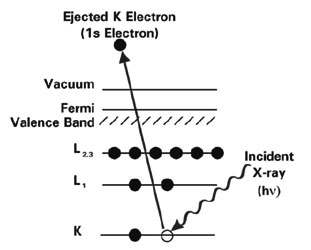
\includegraphics[height=0.3\textwidth]{./images/whatisxps-04.jpg}
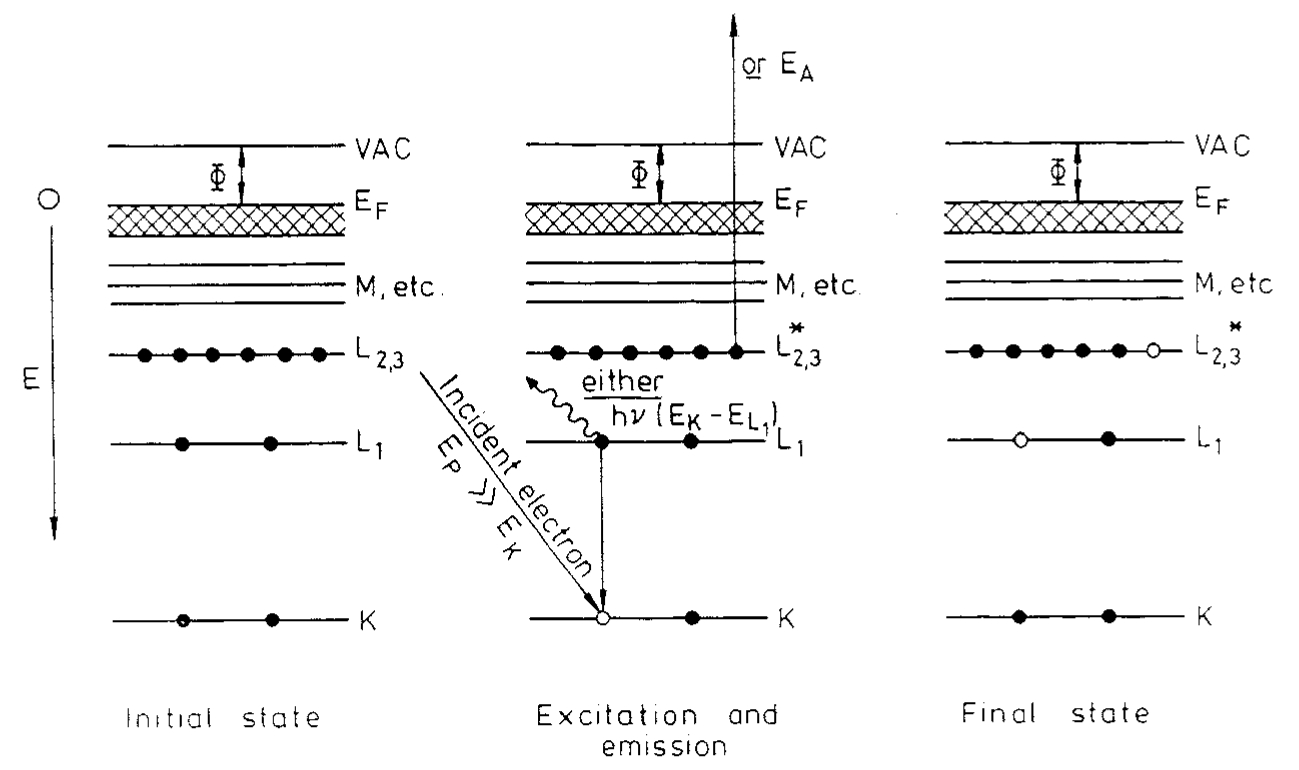
\includegraphics[height=0.45\textwidth]{./images/auger.jpg}
\caption{Shematic diagram of the process of Auger emission in a solid. Taken from \cite{_whatisxps-04.jpg_2015}(left/obove) \cite{Briggs_90}(right/lower)}
\label{fig:auger-core}
\end{figure}

The \index{XPS!chemical surrounding} chemical surrounding of atoms changes their binding energy, making XPS an ideal tool to detect changes in chemial surrounding. Although the analysis is averaged over the area of the incident X-rays (typically hundrets of mircons up to several mm) its results are very precise. This makes it possible to distinguish differently bound atoms within single atomic species and therefore gives rise to otherwise not directly observable processes like growth, intercalation, etching and binding of for example graphene islands on Ir(111)\cite{busse_graphene_2011-1,granas_oxygen_2012}.

With the use of aluminium X-ray sources, electrons are excellerated with typically \SI{15}{\keV} onto the targets. Most of the created radiation goes into the principal characteristic line ($K\alpha_{1,2}$). Higher ones ($K\alpha_{3,4}$, $K\beta$) are also observed but with much lower intensities. In addition there is a continuous background called Bremsstrahlung extending up to the energy of the incident electron energy. This background is of no use for the XPS measurement and has to be substtracted in a more or less artificial way.

For the ease of analysis, many spectra are recorded with monochromatized radiation. This selects a certain energy for the following illumination of the sample. This technique relies on the dispersion of X-rays within a crystal. It is described by the Bragg relation $n\lambda = 2d\sin(\theta)$ where n is the diffraction order, $\lambda$ the wavelength of monochromatized radiation, d the distance between two crystal layers and $\theta$ is the so called Bragg angle. The first order peak for Al $K\alpha$ radiation ($\lambda=\SI{0,83}{\nm}$, $E=\SI{1486,6}{\eV}$) is at $\theta=\SI{78.5}{\degree}$ (using the $10\bar10$ planes of a quartz crystal with $d=\SI{0,425}{\nm}$). Therefore the angle between incident and reflected beam is about \SI{23}{\degree}.\cite{Riviere_90}

The spectra used in this work are recorded without monochromatized radiation as not stated otherwise.

The \index{XPS!binding energies} binding energies of some often observed peaks are given in table \ref{tab:XPS-intensities}
\begin{table}\centering
 \caption{Position and origin of several XPS peaks, taken from\cite{wanger_handbook_1979}}
 \begin{tabular}{llll}
  Eelement & excited state & Binding energy [eV]& comment\\ \hline \hline
  O & 1s & 531&\\
  N & 1s & 398,1&\\
  C & 1s & 285&\\
  B & 1s & 189,4& \\
  Cu & 2p & 953 (1/2), 933 (3/2) & suitable for oxidation analysis\\
  Cu & LMM & 560-580 & suitable for oxidation analysis\\
  Cu & 3s & 123 &\\
  Cu & 3p & 77 (1/2), 75 (3/2) & \\
 \end{tabular}
\label{tab:XPS-intensities}
\end{table}
% \begin{figure}
% 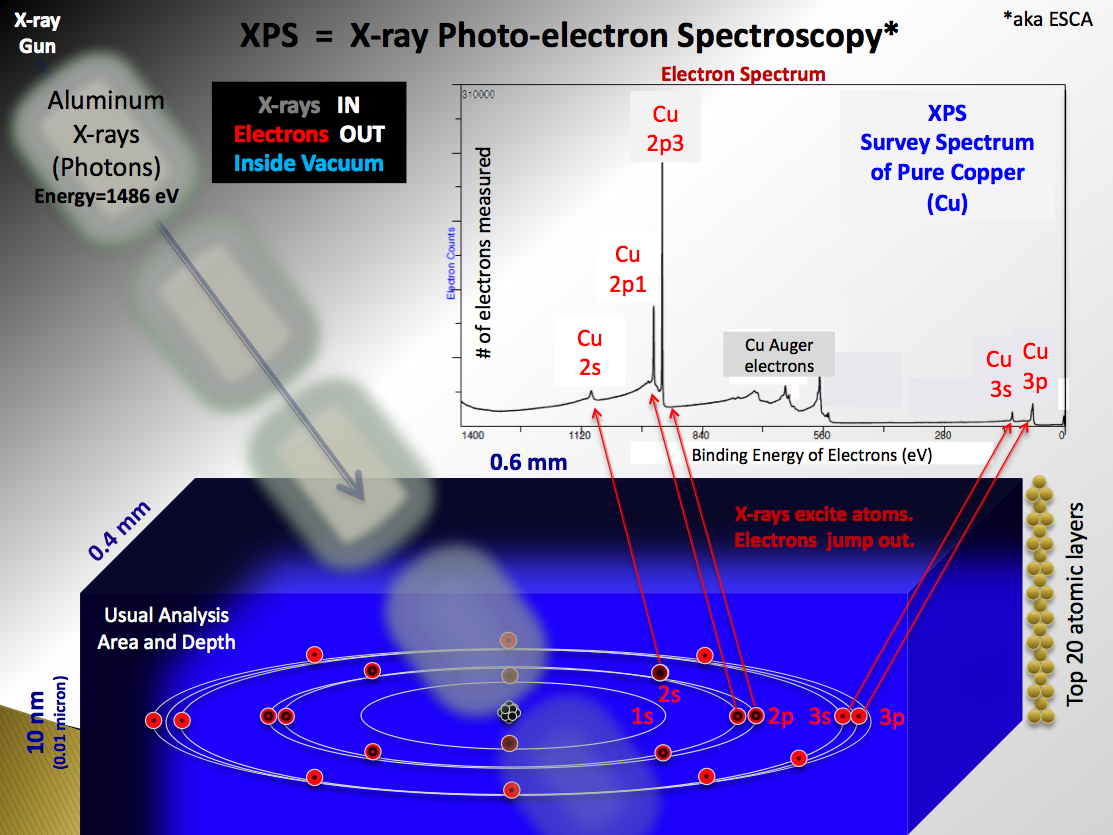
\includegraphics[width=0.7\textwidth]{./images/XPS_PHYSICS.jpg}
% \caption{Sketch of the XPS process. Taken from \cite{_xps_physics.png_2015}}
% \end{figure}
\paragraph{Peak shapes}\index{XPS!Peak shapes}
The shape of the peaks typically resembles the line shape of the used Xrays (Gauss width $\approx 1eV$). In case of s-states (l=0) (B1s, N1s, C1s) the peaks are singulets. With increasing j=l+s, the spin-orbit (j-j) coupling introduces a 'parallel' and 'anti-parallel' nature of the spin, resulting in two different j=1/2(3/2) and therefore two different energies. The split in energy is expected to increase as Z increases (for constant n,l) or as l decreases (n constant). This makes the splitting of 3p orbitals larger than that of the 3d's. The ratio of the two peaks is given by their degeneracy (2j+1).\cite[113]{Riviere_90}
\begin{table}
\caption{Spin-orbit splitting parameters. Reproduced from \cite{Riviere_90}}
\centering
 \begin{tabular}{ccc}
 Subshell & j values & Area ratio \\
 s & $\frac{1}{2}$ & --- \\
 p & $\frac{1}{2}$,$\frac{3}{2}$ & 1:2 \\
 d & $\frac{3}{2}$,$\frac{5}{2}$ & 2:3 \\
 f & $\frac{5}{2}$,$\frac{7}{2}$ & 3:4 \\
 \end{tabular}
\end{table}


\paragraph{experimental setup}
As discussed above, the XPS setup requieres a source of X-ray, an monochromator (optional) and an electron detector that can scan the energy range up to the X-ray energy. The detector selects the energy to be recorded via a \underline{\ \ \ \ \ \ \ \ \ \ \ \ }.
\paragraph{quantitative analysis}
The more atoms of a specific kind are present, the larger the signal gets. Therefore the signal intensity resembles the amount of atoms on the topmost surface layers($\approx \SI{10}{\nm}$).

As each irridiated atomic species has a different cross section for adsorption of X-rays with a certain energy they emit auger and core level spectra with a different intensity. Comparing the cross section of e.g. N with B's, one can see that it it roughly 3-4 times as large (B: \SI{6,87e3}{\barn\per atom}, N: \SI{25,82e3}{\barn\per atom} for $\textnormal{Al} K_{\alpha}$)\cite{henke_x-ray_1993}. Meaning that the signal from the N is much stronger than that of the B, although their number of atoms is equal.

A calibrated XPS is capable of measuring the surface coverage of an adlayer (e.g. BN) compared to the bulk of the sample. Calibration works as follows:
\begin{itemize}
 \item A perfect, full layer of a known material (e.g. C) is prepared (graphene)
 \item The known cross section for C (\SI{6,87e3}{\barn\per atom})\cite{henke_x-ray_1993} relates the signal to the number of atoms of the full layer.
 \item One only has to devide the signal of the unknown coverage (of known material) by the cross section (of C) and directly receives the coverage. Keep in mind that the X-ray penetration depth (and with it the signal of the substrate) stays only constant if the illumination angle stays constant. Even small angular variations may change the signal.
\end{itemize}
Refering to \cite{ertl_low_1986} the fraction $\theta_A$ of an adsorbate A on a surface B can be calculated via
\begin{equation}\label{eq:adlayer-coverage}
 \theta_A=\frac{I_AI_B^0\cdot \exp(\frac{a_A}{\lambda_A}\cos(\Theta))}{I_AI_B^0(\cdot \exp(\frac{a_A}{\lambda_A}\cos(\Theta))-1)+I_BI_A^0\cdot \exp(\frac{a_A}{\lambda_A}\cos(\Theta))}
\end{equation}
where 
\begin{table}[h!]\centering
\caption{Description of parameters used in equation \ref{eq:adlayer-coverage}}
 \begin{tabular}{cc}
  Parameter & Annotation \\ \hline \hline
  $I_A$	& integrated intensity of the adsorbate peak \\
  $I_A^0$ & cross section of element A \\
  $\lambda_A$ & mean free path of electrons in material A \\
  $a_A$ & thickness of adlayer \\
 \end{tabular}
\end{table}
The mean free path of electrons with energy E in a solid is given by $\lambda_M=\SI{0,41}{}\cdot a_M^{\SI{0,41}{}}\cdot E_M^{\SI{0,5}{}} $ where $a_M$ is the atomic size of M. 

Literature:
\begin{itemize}
 \item Photoabsorption cross sections for various elements \cite{henke_x-ray_1993})
  \item oxidation processes of Cu: \cite{deroubaix_x-ray_1992}.
\end{itemize}
  \section{\textbf{A}tomic \textbf{F}orce \textbf{M}icroscopy}
     Introducing STM as a electronical sensitive method to investigate surfaces, the atomic force microscopy interacts in a different way with the sample.
To scan the surface of the sample, one uses an small tip (cantilever) to literally interact with it. Due to its small distance different kinds of forces occure. The force induced movement of the tip is then interpreted an information on the surface may be derived.
The layout of a typical \index{AFM} consists of the cantilever itself and some kind of deflection measurement, typically made of the position-sensitive detector (PSD) consisting of two closely spaced photodiodes whose output signal is collected by a differential amplifier.
Bild: AFM schematic

When the tip moves above the surface it interacts with it due to different forces. These are typically:
\begin{itemize}
 \item van-der-waals interaction
 \item mechanical contact force
 \item capillary forces, chemical bonding, electrostatic forces, Casimir forces, solvation forces and so on
\end{itemize}
A magnetic tip can be used to scan for magnetic forces on the sample surface.

There are several operational modes to drive an AFM:
\begin{enumerate}
 \item \textbf{Contact (static) mode}: The cantilever is operated in contact with the sample surface. At very close proximity, repulsive forces are stronger than the attracting ones. The signal used to gain information on the sample is either the feedback loop to keep the tip at the same absolute position or directly the deflection of the cantilever.
 \item \textbf{Intermittend contact mode (tapping) mode}: While the contact mode has some disadvantages when scanning samples with an adsorbat layer (tip sticks to surface when close ehough to measure short-range forces) another mode has established. Hereby the tip oscillates with amplitudes in the \SIrange{100}{200}{\nm} regime and is not dragged the whole way across the sample. The intermittend forces acting on the tip when reaching the sample are measured. The change in amplitude when in close vicinity to the surface is a sign of the actual height.
 \item \textbf{Non-contact mode}: The cantilever is driven at its resonance frequency with amplitudes smaller than \SI{10}{\nm} and at a certain distance to the sample. Long-range forces like van-der-waals and others change the resonance frequency of the cantilever. This change is a indication of the acting force between cantilever and sample.
\end{enumerate}

\begin{itemize}
 \item AFM produces a true height-profile of the sample (and not a projection of the surface onto a 2D-map like in STM)
 \item Works in ambient pressure and even in liquids
 \item It has limited resolution especially when scanning features steeper than the tip apex
\end{itemize}

Its advantages are the comparable large image size of many hundred \si{\nm} compared to only some dozen \si{\nm} in the case of STM. Scan speeds are typically some orders of magnitude larger than those in STM so that image acquision is much faster.
  \section{\textbf{S}canning \textbf{T}unneling \textbf{M}icroscopy}
     Another commonly used surface sensitive method is the scanning tunneling microscopy (STM). It is as well related to the true topography of the sample, as well as its electronic configuration.

An \index{STM} STM uses the quantum mechnanical tunneling effect. Through the fact that the wave function of a particle does not strictly end within the body it lives in, it is possible to achieve an overlap into the surrounding vacuum. If another material is in a close proximity of the other surface particles can overcome the barrier and cross the vacuum gap - a process known as tunneling. The distance between the two materials is the dominant factor which determines the amount of electrons that are able to tunnel. Assuming the two materials to be the same, the created, time averaged current is zero because the same amount of electrons flow in either direction. If a voltage is applied across the vacuum gap, the current becomes non-zero and flows in a certain direction. This voltage - called bias (voltage) - may be switched and the current has to flow in the opposite direction. This enable detection of either electrons living in the sample (negative bias) or holes (positive bias).
\underline{\ \ \ \ \ \ Bilder: STM-sketch \ \ \ \ \ \ }.

In principle there are two ways to operate an STM. 

First the \textbf{constant current mode}, where the tip is regulated to achieve the very same tunneling current and moved more distant or closer to the sample surface. The information on the sample are the bias voltage and the distance maintained to the sample. 
Second the \textbf{constant height mode} where the tip has always the same absolute height, but as the tip-sample changes the tunneling current varies, which then becomes the measured quantity.
\underline{\ \ \ \ \ \ Bilder: constant height, constant current \ \ \ \ \ \ }.

To avoid crashes when the sample is very irregular, many STM's are operated in constant current mode. Typical tunneling currents are in the range of \SIrange{0.01}{100}{\nA} where the applied voltage may range from \SIrange{0.01}{10}{\volt}.

With the help of STM the reconstructed surface of Si(111) was first discovered \cite{binnig_1983}.

STMs may be operated at very different temperatures. The temperature range is only limited by the availability of sufficient coolants like $^4He$ (boiling point: \SI{4.2}{\K}, \SI{0.36}{\m\eV} thermal energy ($E=kT$)) or a mixture of $^3He/^4He$ where $^3He$ has a lower boiling point of \SI{3.2}{\K}. While low temperature (LT) STMs may be operated with solely Helium, it is more resource-saving to cool the direct proximity of the sample and the STM with He, but to suppress the heat flow out of the He-cryostat with a second surrounding nitrogen cryostat (boiling point: \SI{77}{\K}). This diminishes consumption of globally limited and rather expensive He. To maintain a temperature of \SIrange{5}{7}{\K}, one to two liters of liquid helium are required a day, plus an additional amount of three to four liters liquid nitrogen. Evaporated Helium is reclaimed in a closed circuit with a system of purifying and storage/cooling steps so that only a small amount of Helium escapes the circuit and is lost.
\underline{\ \ \ \ \ \ Bilder: Kryo STM \ \ \ \ \ \ }.

Experiments within these conditions allow sample temperatures down to \SIrange{5}{7}{\K} and obervations not possible at elevated (room) temperatures. Thermal energy is not high enough to let atoms or molecules move on the surface and make them accessible in STM.

Additional information is found in  \underline{\ \ \ \ \ \ \ \ \ \ \ \ }.

STM has a big advantage compared to techniques like XPS, LEED and such, because it offers information on atomic length scales.

While some images encourage the operator to interpret points with high intensity as atoms it is not that trivial. Tunneling current between tip and sample depends on the LDOS of tip and surface and is therefore not implicitly maximised at the atomic positions. It may also vary with the bias voltage applied in a non-trivial manner. Investigation of this behaviuor led to the establishment of a new measurement technique, called scanning tunneling spectroscopy (see section \ref{section:STS}). 

``This results in a non zero tunneling current when the tip is in the lateral neighbourhood of the adsorbate. This contributes to the apparent expansion of the adsorbate print in its STM image compared to the position of its atoms. Interferences between through-adsorbate nd through-space tunneling processes partici- pate to this effect which is orbital-symmetry- and tip-shape-depenaent. A local density-of-states calculation [8,14,28] is not adapted to grasp this effect since he tip is considered far away from the surface. Moreover, in such calculations, the tip radius or the tip-substrate distance is gener- ally optimized to fit the lateral size of the adsor- bate print with the experimental image [8,28].''\cite{sautet_interpretation_1992}.

\paragraph{Angular measurements} The acuracy of a STM is very high. Its spatial resolution goes down to the atomic scale. Due to the fact, that the tips motion is controlled with different piezos, one has to take different elongations in different directions into account. For example, if the STM scans the fast scanning direction just a bit further than the slow scan direction, the resulting image (although pixelwise square) is no longer physically square anymore. Imagine a square (1:1 side ratio, diagonal angle 45\textdegree) where one side is elongated in the image by 5\%. The resulting square (1:1.05 side ratio, diagonal angle 43.6\textdegree) looks square because it has the equal number of pixels in both directions, but it is physically rectangular. The expression used to calculate the uncertainty with known calibration parameters is
$$\Delta \Theta = 45 - \frac{180}{\pi}\cdot\arctan(\frac{1}{1+x})$$ where x is the percentage of one side beeing longer. This results in an uncertainty of 0.3\textdegree(1\%), 1.4\textdegree(5\%, see example above), 2.7\textdegree(10\%). For moderate shear conformality is almost conserved and the uncertainty below 2\textdegree.

\paragraph{One dimensional tunneling}\index{STM!One dimensional tunneling}
Most information in here refers to \cite{bonnell_scanning_1993}.
While the tip (metal) is far away from the sample, their vacuum levels are supposed to be the same. The corresponding Fermi Energies of sample and tip lie below the vacuum level by the amount of their work functions ($\Phi_s$ and $\Phi_t$ for sample and tip respectively). Wavefunctions of electrons within the solids decay exponentially in vacuum, dependend on their energy with respect to the fermi level.
If sample and tip are in thermodynamic equilibrium, their fermi levels are the same. Electrons now face a potential barrier (approximately rectangular) which can be overcome if their energy is high enough and the barrier sufficiently narrow. When a voltage is applied across the tunneling barrier, the energy of the tip-electrons is shifted by $eV$. When a positive bias voltage is applied, electrons tunnel from the tip into unoccupied states in the sample - a negative bias results in a tunneling current in opposite direction. Since states with highest energy have the largest decay lengths in vacuum, most of the tunneling current is determined by electrons within close proximity to the fermi level.

The tunneling current at a given distance is determined by:
\begin{itemize}
 \item The applied voltage
 \item The density of states of electron source and destination
\end{itemize}

Following the model of \index{STM!Tersoff-Hamann} Tersoff-Hamann((1) uniform density of states in the tip, (2) temperature is low, (3) small bias voltage of some mV, (4) waveform of electrons in tip are s-waves) the tunneling current results to 
$$I=32\pi^3\hbar^{-1}e^2V\Phi^2 R^2\kappa^{-4}e^{2\pi R}D_1(E_F)\rho(r_o,E_F)$$ where $D_1$ is the density of states per unit volume of the tip, R the tip radius and $\rho(r_0,E_F)$ the Fermi-level density of states in the sample. If I is held constant one can see that the tip in principle follows a contour of constant Fermi-level density of states, measured at the center of the curvature of the s-wave like tip. While its a good first approximation of the system, in many cases the bias is much highger than 10mV (\SIrange{1}{5}{\V}) more than just the electrons near fermi contribute.

Using \index{STM!WKB} WKB theory the tunneling current is given by
\begin{equation}
I=\int_0^{eV}\rho_s(r,E)\rho_t(r,eV+E)T(E,eV,r)dE
\label{WKB}
\end{equation}
where $\rho_s(\rho_t)$ is the density of states of the sample (tip) and T is the tunneling transmission probability
\begin{equation}
T(E,eV)=exp\left(-\frac{2Z\sqrt{2m}}{\hbar}\sqrt{\frac{\Phi_s+\Phi_t}{2}+\frac{eV}{2}-E}\right)
\label{Transmission-function} 
\end{equation}
If $eV<0$ the tunneling current is largest for $E=0$ (electrons on the Fermi-level of the sample), if $eV>0$ the tunneling current is largest for $E=eV$ (electrons of Fermi-level in tip).

Due to the fact that it is proportional the the density of states in the tip AND the molecule one can deduce the band structure within a range of several volts in the vicinity of the Fermi ernergy.

This is in line with the assumption that waves of electrons decay expotentially, having the most energetic electrons the largest decay length.
     \subsection{\textbf{S}canning \textbf{T}unneling \textbf{S}pectroscopy}
	\label{section:STS}
First changes of the tunneling current with the bias voltage were observed by Tromp et al. in 1986 \cite{tromp_atomic_1986}. They discovered a change in contrast when scanning a SI(111) surface with either positive or negative bias. The change in contrast is most apparent in semiconductors and semimetals\cite{bonnell_scanning_1993}, but adsorbats and charged areas of the sample change the DOS locally and therefore the contrast in STM.

The vanishing lateral movement of molecules in LT-STM makes them also accessible to tunneling spectroscopy. It is possible to deduce the electronic configuration on with atomic spatial resolution.
\paragraph{Modulating STM}
Spectroscopic information (information on the DOS) can be obtained by either changing the bias voltage [I(V,z)-spectroscopy] or the tip-sample distance [V(z)-spectroscopy].
While simple results may be already obtained when comparing two images recorded at different voltages, more detailed information can be achieved. A constant current image at a certain bias voltage is recorded. If the bias is then modulated with a sinus like waveform, one can extract the differential conductance ($\frac{dI}{dV}$). 
One provides a high frequency (much larger than feedback loop frequency of 1-2 kHZ), low amplitude modulation of the DC bias voltage. The AC part of the tunneling signal is than recorded with a lock in amplifier. The in-phase component is directly the $dI/dV|_{V=V_{bias}}$, recorded simultaniously with the topography. If the modulation frequency is too low, the feedback tries to compensate the modulation by changing the distance to the sample.
If the modulation frequency is too high, the capacitance between tip and sample leads to an $90\deg$ phase shifted current which increases with modulation frequency. One useally chooses the modulation freqeuncy slightly above the cutoff frequency for the feedback loop.

\paragraph{Bias below work function}
If tunneling conditions are such that $eV\leq\Phi$, observed features in $dI/dV$ are associated with the surface DOS. Critical points in the surface projected DOS give rise to features in $dI/dV$. Interpretation of these features with the WKB theory (i.e. differentiating equation \eqref{WKB}) gives
$$dI/dV=\rho_s(r,eV)\rho_t(r,0)T(eV,eV,r)+\int_0^{eV}\rho_s(eV)\rho_t(r,E-eV)\frac{dT(E,eV,r)}{dV}dE$$
The first term contains the DOS of the sample and tip and the transmission function. While it is usually unknown, a closer look to \eqref{Transmission-function} indicates a smooth, monotonically increasing function in V. This mannered dependence on V gives a smooth background described by the second term $\int_0^{eV}\rho_s(eV)\rho_t(r,E-eV)\frac{dT(E,eV,r)}{dV}dE$.
Because T is smooth and monotonic the first term $\rho_s(r,eV)\rho_t(r,0)T(eV,eV,r)$ introduces the dependence on the DOS in the sample for energies $eV$ - our desired spectrum.

If $dI/dV$ is recorded simultaniously with the topography, another contribution arises. One usually observes an decrease in atomic corrugation when the distance between tip and sample is increased. The surface looks flat. To have the same tunneling current on atom positions and in between, the decay length in the valleys $\kappa_v$ must be larger than on the atom positions $\kappa_a$. The Z-dependend corrugation given by Tersoff is $$\Delta(Z)\approx \frac{2}{\kappa}e^{-\frac{\pi^2Z}{a2\kappa}}$$ where a is the lattice constant and $\kappa$ the inverse decay length. To make both a flat looking surface one gets the expression
$$\kappa_v=\kappa_a-\frac{2\pi^2}{\kappa a^2}e^{-\frac{\pi^2\bar Z}{a2\kappa}}$$ 
As the transmission factor changes with the decay length, the tunneling current and with it the $dI/dV$ changes. This is the origin of topographic features in $dI/dV$ maps when recorded at constant current.

The origin of the strongly voltage dependend background can be found in WKB theory as well.
When writing the tunneling current as 
$$ I=\int_0^{eV}\rho_s(r,E)\rho_t(r,eV+E)exp\left(-\frac{2Z\sqrt{2m}}{\hbar}\sqrt{\frac{\Phi_s+\Phi_t}{2}+\frac{eV}{2}-E}\right)dE $$
the tunneling current reduces to 
\begin{equation}
\bar I=\rho_s\rho_t \bar V exp\left(-\frac{2\sqrt{2m}}{\hbar}\sqrt{\Phi}Z\right)
\label{tc}
\end{equation}
Assuming that DOS of tip and sample $\rho_t/\rho_s$ are constant, as well as discarding the change of the tunneling barrier with the bias voltage(an assumption only valid for very small voltages with $eV<<\Phi$) the derivative of \eqref{tc} is given by
$$\frac{dI}{dV}=e\rho_s\rho_texp\left(-\frac{2\sqrt{2m}}{\hbar}\sqrt{\Phi-\frac{eV}{2}}\right)Z$$
Substituting Z with the one obtained by \eqref{tc} leads to $dI/dV= \bar I / \bar V$ - which diverges as  $1/V$ when going to very low bias voltages and gives another contribution to the background. This makes it hard to observe features in close proximity to the fermi level ($V_{bias}=0V$). This background can be reduced when oparating at constant resistance and not at constant current. When doing this, features usually obscured by the $1/V$ diverging background can be observed.

For normalization and interpretation of data, see \cite{bonnell_scanning_1993}.
Normalization is done as argued by\cite{feenstra_tunneling_1987} because of the diverging part at \underline{\ \ \ \ \ \ 0V \ \ \ \ \ \ }.

\paragraph{Bias above work function}
If the bias voltage is higher than the work function of the sample $dI/dV$ reflects mainly states that arise from interaction of electrons at the surface with the polarization they induce in the bulk. Electrons are trapped by this interaction in a region near the surface leaving their lateral movement undistorted. These waves either do interfere con- or deconstructively at the surface. Which type of interference occurs is determined by the applied bias voltage that alternates the bounding condition. The transmission alternates when going from contructive to destructive interference and therefore the tunneling current changes when changing V. 
As an interesting fact, Becker et al.\cite{becker_electron_1985} found that that numerical integration of Schr\"odingers equation could be used together with $dI/dV$ spectra to calculate the absolute distance between tip and sample - an value hard to come by with other methods.

\paragraph{Barrier height measurements from I(Z) spectroscopy (work function difference)}\index{STS!Barrier Height}
Further information can be drawn from the tunneling system when the barrier height may be determined.
Taking the limit of the transmission function \eqref{Transmission-function} for low bias voltage ($eV\approx0$, $E=E_F$) results in 
$$T=exp\left(-\frac{2Z\sqrt{2m}}{\hbar}\sqrt{\frac{\Phi_s+\Phi_t}{2}}\right)$$
Using this in the WKB approximation \eqref{WKB}, one gets $$\frac{dI/dZ}{I}=\frac{2\sqrt{2m}}{\hbar}\sqrt{\Phi_s+\Phi_t}$$
As the work function of the tip usually stays constant, lateral variations in the barrier height can be boiled down to local changes in the work function. This is done by \cite{jia_variation_1998}.

Determining the barrier height in this way often results in to low values for the work function. Discussion of this is found in \cite[96]{bonnell_scanning_1993}.


\paragraph{Resolution}\index{STS!Resolution}
The resolution of STS is determined by the range of energies electrons have when contributing to the tunneling process. This range is $eV$. When $T>0$ the DOS is smeared out and is described by $$f(E)=\frac{1}{1+exp\left(\frac{E-E_F}{kT}\right)}$$ 
Since electrons from occupied states (DOS is Fermi distributed) tunnel into unoccupied states the transmission function has the structure $$T(E,eV,T)=T(E,eV)f(E)[1-f(eV-E)]$$ 
When looking at the shape of the Fermi distribution one can see that most of the electrons participating in the tunneling process arise from a rather narrow area around the Fermi level of the negatively biased electrode (broadening of fermi edge at $T=300K\hat=\SI{0.026}{\eV}$. Electron distribution of tip and sample are broadened by $2 k_b T=\SI{0.054}{\eV}$ thus the energetic range where electrons may come from is \SI{0.1}{\eV}. From the uncertainty relation $\Delta x \Delta k \geq 1/2$ and the dispersion relation for metals $$ \Delta E\ge \frac{\hbar^2k_F}{2M^*\Delta x}=0.47\frac{E_F-E_0}{rk_F} $$\cite{chen_introduction_2008}. ``The asymmetric form of $T(E,eV)$, with the sharp inscrease at $E_F$, helps to make the effective resolution of the STM somewhat higher when probing empty states of the sample than when probing filled states.''
The resolution at room temperature is \SI{140}{\m\eV}\cite{hansma_tunneling_1982}.
As the tunneling transmission is always a factor of the tip and sample DOS, STS is always limited to the unknown electronic structure of the tip. While geometry at the tip apex is successfully enhanced with field evaporation techniques its electronic structure may differ greatly from the bulk one due to unusual bonding geometry and small size. Some\cite{tersoff_role_1990,ciraci_tip-sample_1990,lawunmi_theoretical_1990,kobayashi_simulation_1990} groups have calculated band structures for different tips and their influence in the tunneling process.


\paragraph{Other methods with STM}Inelastic tunneling => vibrational states resolvable => chemical descicive measurements; Tip induced band bending

\paragraph{Gundlach oscillations}
Gundlach was the first who calculated transmission currents for trapezial potential barriers \cite{gundlach_zur_1966}. The oscillations named after him are due to standing wave states in the potential tip-sample potential barrier \cite{binnig_tunneling_1985,becker_electron_1985}
``When the Fermi level of the tip is close to the vacuum level of  the  sample,  the  contribution  of  the  image  potential  is significant. The superposition of the  image  potential  and the electrostatic  potential forms a specific potential well, and the lowest-order peak is a Gundlach oscillation related to a standing-wave state in this well. When the Fermi level of the tip is higher than the vacuum level of the sample, the image potential becomes negligible, and the potential well can be  approximated  by a triangular  shape. Those peaks beyond the lowest-order peak are the Gundlach oscillations related to the standing-wave states in the triangular well. Derivation  based  on  quantum  mechanics  shows  that  the energy difference of the standing-wave states in the triangular  well  is  proportional  to $F^{2/3}$,  where F is  the electric field in the tip-sample gap''\cite{lin_manifestation_2007}
  \section{\textbf{S}canning \textbf{E}lectron \textbf{M}icroscopy}
     Invented in the 1930's by Manfred von Ardenne\cite{ardenne_elektronen-rastermikroskop_1938}, Scanning electron microscopy (SEM)\index{SEM} is another versatile tool for the experimentalist. In contrast to (LT-)STM and AFM, SEM is capable of imaging huge areas of the sample within a very short time, which allows for a vast overview as well as good statistics. Magnifications reach up to 500k and above, illustrating even features in the order of \SI{1}{\nano \meter}.

As the name already discloses, SEM scans the surface with electrons. Their interaction with the material are diverse and some of them are explained in the following. While all effects are present in every measurement, not every microscope features detectors for all of these. While detectors for secondary electrons are standart equipment others may be not.

\begin{itemize}
 \item \textbf{Secondary electrons (SE)} are produced in the bulk by the high energetic primary electon beam within close proximity to the surface. This is why SEMs offer a very good resolution of the surface itself.
  \item \textbf{Backscattered electrons (BSE)} are elastically scattered primary electrons. The resolution of this mode is not as high for the secondary electrons. The intensity of the BSE depends strongly on the the atomic number Z of the specimen. It is useful for a complementary view, for example when chemical composition is of high interest.
  Electron backscatter diffraction (EBSD) is used to achieve information on the crystallographic structure of a specimen.
 \item \textbf{Characteristic X-Rays} are used to identify the composition and measure the abundance of elements in the sample, too. See section \ref{sec:XPS} and figure \ref{fig:auger-core} therein for more details.
 \item \textbf{Cathodoluminescence (CL)} happens when electrons hit a material and exite photons. This effect is used in televesion screens where high energetic electrons are accelerated onto a screen containing phosphorus. There they distribute their energy with many others, some of those loose energy in form of photons which wavelenghts are within the visible spectrum. These light is called cathodoluminescence.
 \end{itemize}

The primary electrons are created with a filament. These often consist of tungsten (metal, high melting point, low work funtion). Alternatives are lanthanum hexaboride ($\textnormal{LB}_6$) - often used in LEED setups, too - or zirconium oxide.
Electrons are accelerated (typical energies are within \SIrange{1}{40}{\kilo \eV}) and focused on the specimen surface in a spot with few \si{nm} diameter with condenser lenses. Scanning the surface is achieved with coils that deflect the electron beam and therefore the actual scanning spot.

When the electrons hit the surface, they interact with the specimen in a small volume. The volume depends on the electron's energy, the atomic number Z of the specimen and the specimen's density. It is typically in the order of \SIrange{0.1}{5}{\micro \meter}.

Drawbacks:\\
\begin{itemize}
 \item[-] Sample has to be mounted $\rightarrow$ no in-situ measurement, surface alteration in between
 \item[-] Rather ``dirty'' vacuum $\rightarrow$ surface alteration while measuring
 \item[-] Measurement destroys sample $\rightarrow$ adsorbat build-up due to chemical reaction below e-beam
\end{itemize}


  \section{\textbf{L}ow \textbf{E}nergy \textbf{E}lectron \textbf{D}iffraction}
     Low energy electron diffraction (LEED)\index{LEED} is a technique for the determination of surface structures. It uses an electron beam $0.5mm$ with low energies ($\leq \SI{500}{\eV}$) which is scattered from the surface and creates an diffraction pattern. The shape of this pattern is then related to the surface geometry. Note that although a sharp LEED diffraction pattern may be observed, the area of coherently scattering electrons is about \SI{20}{\nm}. Thus a small region on the illuminated sample has to be ordered in order to show diffraction patterns. This does not mean that the whole sample is ordered.

% It may be used qualitatively to determine orientation and size of an absorbat with respect to the substrate by the position of the diffraction spots\cite{tang_growth_2002}. It is also suitable to gain accurate information on elevation and rotation angles of surface grains\cite{kraus_towards_2013} and corrugation amplitudes.

Lets us first consider an easy model. Electrons from the gun penetrate the sample surface and interact with the solid. Where the interaction is not important one may consider an exponential decay in direction of propagation:
$$I(d)=I_0\cdot e^{-\frac{d}{\Lambda(E)}}$$ where $I$ is the intensity in penetration depth d and $\Lambda(E)$ is the inelastic mean free path of electrons. It depends on their energy E, but is not so sensitive to the material itself in this energy range. It is typically between \SIrange{5}{20}{\angstrom} for energies \SIrange{20}{200}{\eV}. This is why LEED is more surface than bulk sensitive.

\subsection{Single (elastic) scattering theory}\index{LEED!elastic scattering}
As electrons are particle and wave at the same time, they have a \index{de Broglie} de Broglie wave length $\lambda$:
$$\lambda=\frac{h}{\sqrt{2mE}} \qquad \lambda[nm] \approx \sqrt{\frac{1.5}{E[eV]}}$$
Considering a real space lattice {$\vec a_1,\vec a_2,\vec a_3$}, scattering is described in reciprocal lattice more conveniently. Transforming the basis set $\vec a_i$ to its corresponding reciprocal basis set 
$$\vec k_i=\frac{2\pi \vec a_{i+1}\times\vec a_{i+2}}{\vec a_i\cdot(\vec a_{i+1}\times \vec a_{i+2})}$$ with $a_i \in [0,1,2,3]$.
The Laue condition (Bragg's theorem in reciprocal space) $$\vec k-\vec k_0 = \vec G_{hkl}$$ with $$\vec G_{hkl}=h\vec k_1+k\vec k_2+l\vec k_3$$ describes conditions for an incident beam $\vec k_0$ and its diffracted equivalent $\vec k$. Remember that the penetration depth is so small, that there are only enough contributing scattering partners for directions parallel to the surface. Therefore Laues condition reduces to surface parallel ($\parallel$) components of $\vec k$ $$\vec k^{\parallel}-\vec k^{\parallel}_0=\vec G_{hk}=h\vec k_1 + k \vec k_2$$ To visualise the possible diffraction conditions of a surface one can use the Ewald's sphere construction.
\paragraph{Ewald's sphere}\index{LEED!Ewald's sphere}
By depicting the surface as an infinitely extended 2D-array of dots seperated by $h\vec k_1$ in one and by $k\vec k_2$ in the other direction, one chooses an incident beam $k_0$. It is drawn such that it ends on the reciprocal lattice plane. Then one draws a circle around this point with radius $r=|k_0|$ (energy conservation). Now extend the reciprocal lattice points of the surface to rods perpendicular to the surface. Every vector from the origin of the circle and the intersection of circle and rod is an allowed diffracted beam. 

When increasing the energy, the radius $|\vec k_0|$ more and more rods contribute and get visible on the screen. If the energy is high enough, one can see the high order laue zone where diffraction spots form a dense ring-shaped feature.
\begin{figure}[h!]\label{ewald-sphere}
 \centering
 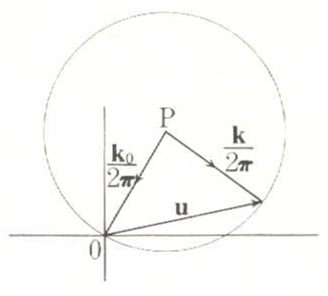
\includegraphics[height=6cm]{./images/ewald-sphere.jpg}
 \caption{ewald-sphere, ``top'' view, taken from \cite[109]{cowley_diffraction_1981}}
\end{figure}

\begin{figure}[h!]\label{LEED}
 \centering
 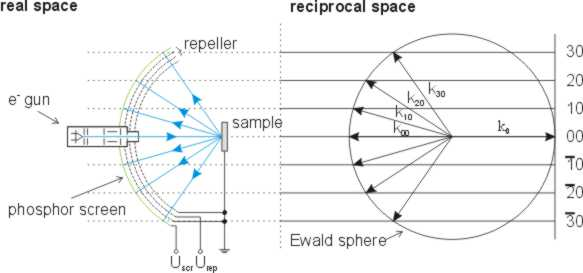
\includegraphics[height=6cm]{./images/ThreeGridLeed.jpg}
 \caption{ewald-sphere, ``side'' view, taken from \cite{threegridleed.jpg_2015}}
\end{figure}

For electrons with energies of \SI{0.04}{\eV} the diameter of the ewald sphere will be \SI{50}{\per \angstrom} in reciprocal space f. On this sphere only a small region of radius \SI{5}{\per \angstrom} will contain the small angle scattered waves of LEED.

\paragraph{Structure factor}\index{LEED!Structure factor}
Consider a function that describes the atomic positions in real space $\phi(\vec r)$. Let it be integrable, when one defines the Fourier transform such that 
\begin{equation}\label{eq:structure_factor}
\phi(\vec k)=\int_{\vec r} \phi(\vec r)e^{-i\vec k \vec r}d\vec r 
\end{equation}
If one chooses $\phi(\vec r)$ to resemble the form of the scatter partners as well - like $\phi(\vec r)=f(\vec r)\circ \sum_{j=1}^N\delta(r-R_j)$ where $R_j$ are the atom positions in real space and $f(r)$ describes the form of the atom. $\circ$ shall represent the convolution product, i.e. $FT(\phi(\vec r))=\phi(\vec k)=f(\vec k)\cdot \sum_{j=1}^N e^{-i\vec k \vec R_j}$ As the intensity $I(\vec k)\varpropto |\phi(\vec k)|^2$
$$\langle I(\vec k) \rangle \varpropto 
\langle |\phi(\vec k)|^2 \rangle =
\langle |f(\vec k)|^2 \left( \sum_{m=1}^N e^{-i\vec k \vec R_m} \right) \left( \sum_{n=1}^N e^{i\vec k \vec R_n}
\right) \rangle=|f(\vec k)|^2 \underbrace{\langle \left( \sum_{m,n=1}^N e^{i\vec k (\vec R_n-\vec R_m)} \right) \rangle }_{S(\vec k)}$$

One can calculate different structure factors for different lattices. As used crystals are fcc lattices, their basis set $R_j$ is 
$$ \vec{R}_0 = \vec{0} \quad
 \vec{R}_1 = (a/2)(\vec{a_1} + \vec{a_2})\quad
 \vec{R}_2 = (a/2)(\vec{a_2} + \vec{a_3})\quad
 \vec{R}_3 = (a/2)(\vec{a_1} + \vec{a_3})$$ with indices given by (1/2,1/2,0), (0,1/2,1/2), (1/2,0,1/2).

Following the definition of \eqref{eq:structure_factor} above, one gains an relation of $\vec {k}=(h,k,l)^T$ that describes the structure factor. Exchanged $\vec k$ with $\vec q$ in the calculation for clarity.
\begin{align*}
S_{\vec{q}} &=  f \left[ e^{-i\vec{q}\cdot\vec{0}} + e^{-i\vec{q}\cdot(a/2)(\vec{a_1} + \vec{a_2})} + e^{-i\vec{q}\cdot(a/2)(\vec{a_2} + \vec{a_3})} + e^{-i\vec{q}\cdot(a/2)(\vec{a_1} + \vec{a_3})} \right] \\
&= f \left[ 1 + (-1)^{h + k} + (-1)^{k + l} + (-1)^{h + l} \right] \\
&=  \begin{cases} 4f &\mbox{h,k,l all even or all odd}\\
                  0 &\mbox{mixed parity} \end{cases}
\end{align*}
This means, that only diffractions with $S_{\vec q}\neq 0$ contribute to the diffraction pattern. For fcc lattices, only sets of all even or all odd (h,k,l) create the pattern. 

For bcc its $$ \vec{R}_0 = \vec{0} \quad
 \vec{R}_1 = (a/2)(\vec{a_1} + \vec{a_2}+ \vec{a_2})$$ and thus 
 $$(h,k,l)=\begin{cases} 2f &\mbox{h,k,l all even}\\
                  0 &\mbox{h,k,l all odd} \end{cases}$$ due to the different basis.

In general, the structure factor is a imaginary quantity. It has the form $S(\vec k)=F_{hkl}e^{-i\alpha_{hkl}}$. $F_{hkl}$ describes the superpositioned amplitudes, while $\alpha_{hkl}$ is the phase of the resulting scattered wave. One can think of it, like having the same atoms on a crystal plane (hkl) scattering the incoming wave, with the same amplitude for each equal atom and the same phase. Now consider a parallel plane (hkl) with the same plane distance but occupied with another set of the same atoms. Since these planes are parallel Braggs law is fulfilled, the incident wave gets scattered but with a phase shift that depends on the two plane's separation. The structure factor takes these planes into account and adds the two scattered waves into one. Since these planes are created by the basis of the crystal, one just needs to know the single atom's distance to the initial plane (arbitrarily chosen atom, mostly $\vec 0$) to calculate the structure factor. If atoms are not the same, i.e. their scattered amplitude is not the same, the structure factor adapts with different $f_i$'s for different atomic species. Further reading into computational efforts and such can be done in ref. \cite{van_hove_surface_1979}.

Further reading into determining overlayer distances and structure of S on Ni can be found here \cite{demuth_small_1973,duke_structure_1973,andersson_surface_1972}
\paragraph{Temperature correction}\index{Debye-Waller factor}
Corrections have to be made if thermal motion is included. A solid with temperature $T$ has some kinetic energy which makes the atoms able to oscillate around their central position $R_j$. If one replaces $R_j$ in the calculation above with some time dependend value $\vec r_i(t)=\vec r_{i,0}+\vec u_i(t)$, with fast changing function $u(t)$ describing the dislocation from the ideal position, one yields:
$$ \langle S(\vec q) \rangle =\sum_{i}f_{i}\,\langle\exp\left[i\,\vec{q}\cdot\left(\vec{r}_{i.0}+\vec{u}_{i}(t)\right)\right]\rangle=\sum_{i}f_{i}\,\exp\left[i\,\vec{q}\cdot\vec{r}_{i.0}\right]\,\langle\exp\left[i\,\vec{q}\cdot\vec{u}_{i}(t)\right]\rangle $$
Expanding the exponential function to terms $\leq 2^{nd}$ order 
$\langle \exp\left[i\,\vec{q}\cdot\vec{u}_{i}(t)\right] \rangle \approx 1+i\,\langle \vec{q}\cdot\vec{u}_{i}(t)\rangle-\frac{1}{2}\langle\left(\vec{q}\cdot\vec{u}_{i}(t)\right)^2\rangle$ where the first term equals zero because $\langle \vec{u}_i(t)\rangle=0$ (vibration around center).

$$\langle \left(\vec{q}\cdot\vec{u}_{i}(t)\right)^2 \rangle=|\vec{q}|^{2}\,\langle|\vec{u}_{i}(t)|^2\rangle \,\langle\cos^{2}\theta\rangle$$ The time avarage 
$$ \langle \cos^{2}\theta \rangle=\frac{\int_{0}^{2\pi}\mathrm{d}\phi\int_{0}^{\pi}\mathrm{d}\theta\,\sin\theta\cos^{2}\theta}{\int_{0}^{2\pi}\mathrm{d}\phi\int_{0}^{\pi}\mathrm{d}\theta\,\sin\theta}=\frac{1}{3} $$ inserted into the expansion results in
$$\langle \exp\left[i\,\vec{q}\cdot\vec{u}_{i}(t)\right]\rangle \approx1-\frac{1}{6}\,|\vec{q}|^{2}\,\langle|\vec{u}_{i}(t)|^2\rangle \approx \exp\left[-\frac{1}{6}\,|\vec{q}|^{2}\,\langle|\vec{u}_{i}(t)|^2\rangle \right]$$
Put it in the definition of $\langle S(\vec q) \rangle$ results in
$$\langle S(\vec q) \rangle =\underbrace{\sum_i f_{i}\,\exp\left[i\,\vec{q}\cdot\vec{r}_{i,0}\right]}_{S_0(\vec q)}\,\exp\left[-\frac{1}{6}\,|\vec{q}|^{2}\,\langle|\vec{u}_{i}(t)|^2 \rangle \right]$$
Time averaging the intensity yields $$\langle I \rangle \propto \langle S(\vec q)\rangle^2 =S_0^2(\vec q)\,\exp\left[-\frac{1}{3}\,|\vec{q}|^{2}\,\langle|\vec{u}|^2\rangle \right]=I_{0}\underbrace{\exp\left[-\frac{1}{3}\,|\vec{q}|^{2}\,\langle|\vec{u}|^2\rangle \right]}_{DWF}$$
\begin{itemize}
 \item This means the higher the amplitude of displacements (higher T), the weaker the overall intensity of the spots. This is consistant with the idea that the higher the temperature, the higher the decoherence between two areas. This reduces the intensity.
 \item The DWF reduces the intensity for peaks $|\vec q|>0$ so that peaks with high $|\vec q|$ have less intensity than those with small $|\vec q|$. For initial reading and detailed calculations see \cite{debye_interferenz_1913}.
\end{itemize}
The attenuation of intensity from the DWF can be used to investigate oscillating dislocations of surface atoms. As one would expect the kinetic energy from a vibration with force constant D (harmonic oscillator) to be $D\langle u^2\rangle$, its thermal energy is $k_bT$. When now the atom faces a missing surface layer (and therefore becoming itself one) the atoms left to share energy with lie in the same plane or below. It one assumes pairwise interaction one would expect $D$ to be halfed or $\langle u^2 \rangle$ compared to a intact pair of atoms\cite[69]{woodruff_modern_1986}. Although vibrations may be accessible in LEED it is not well suited to adress this question. As other studies indicate the effect of enhanced amplitudes is most dominant at the very surface and - due to the fact that LEED probes several layers - it may average $\langle u^2 \rangle$ over the first 3-5 layers.

One may look deeper into what causes scattering when electrons face atoms. The coulomb interaction is strong and electrons get scattered depending on the electron density of the atom. So if one knew both the amplitude and the phase of the scattered electrons, one could calculate the electron densities. Since the phase can not be obtained a workaround has to be chosen such that one has a relative measurement of the in- and outcoming phases. If one adds an electronically denser item (like a metal atom) in the crystal it will change the diffraction pattern and one may derive the phases from that. Same is done with molecules, where one compares an already resolved scattering pattern with the ``new'' one to track changes and calculate the phase.

Another (quantum mechnanical) description can be found in \cite[341]{liuksiutov_two-dimensional_1992}.

\paragraph{Spot shapes and changes} to them are given in \cite[36]{woodruff_modern_1986}, along with a detailed error evaluation. It describes under witch condition peak splitting may occur and gives examples for peak splitting related to domain boundaries and different atomic ordering on surfaces. If the surface is made of vicinal steps (i.e. 100 steps with 111 terraces, like 532) one can see 
\begin{itemize}
 \item The lattice of the substrate (in this case the unit cell contains the step distance and height)
 \item Splitted LEED spots which arise from the kinked surface and the periodic defect step formation on the ctystal\cite[37ff]{riemann_ionic_2002}.
\end{itemize}

\paragraph{Friedel's law}\cite[93]{cowley_diffraction_1981}
Provided that for the electrons no absorption effect is important, the electron desity $\rho(\vec r)$ may be assumed to be a real function satisfying \begin{align}
F(-\vec u) &= \int \rho(\vec r) \exp{[2\pi i(-\vec u)\vec r]} d\vec r \\                                                                                                                                                      &=F^\star(\vec u)                                                                                                                                                      \end{align}
As the intensities scale with $I=|F|^2$ it follows that inversion of a crystal through a center of symmetry does not change the diffraction intensities in a kinematical (single scattering) approximation. Since the inversion of \eqref{eq:structure_factor} gives the electron density $$\rho(r)=\int F(\vec u)\exp{[-2\pi \vec u \vec r]} d\vec u$$ If the diffraction amplitudes could be measured so that $F(\vec u)$ could be derived, than $\rho (\vec r)$ can be calculated by evaluating the integral numerically. But measurement of the wave amplitudes $F(\vec  u)$ is not possible, only the intensities $FF^*$ are recorded. Thus information on the phases is lost and $\rho(\vec r)$ not calculable.

\paragraph{superstructure determination}
\underline{\ \ \ \ \ \ \ \ asd \ \ \ \ \ \ \ \ \ }
\subsection{Multiple scattering theory}See \cite[55]{woodruff_modern_1986} for concepts of modelling, \cite{van_hove_surface_1979} for explaining the calculations.

The incident beam of coherent (waves have equal phases) electrons are diffracted under the fulfillment of Laue's law to result in coherent radiation on the LEED screen. Above only single scattering event were taken into account but the interaction of electrons and solid is much more pronounced than for example for X-rays. So electrons scattered once will be able to scatter a second or third time, following again Laue's law. This implies scattering on the very same oriented crystal planes. Then the phases are uniquely defined and the waves amplitudes are added. This is referred to as ``dynamical'' scattering. So if the crystal has some impurities, grainboundaries and such, scattered electrons will be attenuated. Multiple scattering therefore gives an indication on the purity of the crystal itself. On the other hand, if atomic ordering does not extend over areas required for defined scattering the relative phases of each ordered crystal domain will add up randomly and their amplitudes are added incoherently. This is referred to as ``multiple elastic scattering''.

As a comparison, the path length for X-rays to be scattered multiple times is $\approx \SI{1}{\micro \meter}$, serveral times longer for neutrons and only one or two hundert \si{\angstrom} for eletrons\cite[90]{cowley_diffraction_1981}.

\paragraph{Resolution and difficulties}
I real world experiments, there is often a spread in incoming wave momenta and the problem of focus. 
\textbf{Finite Sources - Ewald shell emergence}
For LEED witch magnetic focus, the angle of convergence may be chosen as high as \SI{E-3}{\radian}(within magnetic lenses of an tunneling electron microscope). But even within this small range of angles, the appearence of the ewald sphere changes. If one chooses two different angles for incoming waves $\vec k_0$ the waves scatter in different directions resulting in a blurring of diffraction spots.

\paragraph{Wavelength spread}
For electrons a nearly monochromatic radiation with line widths of about $10^{-6}\lambda$ are achieveable (1981). The spread of wavelengths in the incoming beam modifies the length of the $\vec k_0$ and as a result the diffracted spot shapes change from spots to lines variing as well in orientation as in length\cite[113]{cowley_diffraction_1981}``beeing small and parallel to $\vec k_0$ in the limit of small scattering angles; of medium length and roughly perpendicular to $\vec k_0$ like for intermedium scattering angles and of maximum length and oppositely directed to $\vec k_0$ for scattering angles of \SI{180}{\degree}''.

Adding this effect to the finite source problem, one ends in a complicated scattering volume. Thus the relationship of the observed intensity to the function $|F(\vec q)|^2$ is only to derived by calculation from a detailed model containing the parameters of the experimental system.

For some examples of vacancy deviations, see \cite[144-151]{cowley_diffraction_1981}.
In LEED, if the size of diffraction elements are smaller than the width of the transfer function, one observes broadening in the peaks and therefore makes it able to access their size\cite[40]{liuksiutov_two-dimensional_1992}.


  \section{\textbf{C}hemical \textbf{V}apor \textbf{D}eposition}
        %  this is a description of a cvd process usually used in this worl
There are two major ways to grow adlayers defined by their atomic constituents and certain stoichiometry in UHV, namely the chemical vapor deposition (CVD) or temperature programmed growth (TPG) of a precourser.

While the latter works by adsorption of the precourser onto the surface where it schould grow and activating the reaction via heating, the first uses a already hot surface to decompose the precourser on. 

\paragraph{CVD}\index{CVD}offers some advantages over TPG when it comes to homogenous growth of a monolayer. The precourses decomposes on contact with the hot substrate surface and its fragments for the adlayer. As time goes by, the adlayer grows in coverage and less free hot surface area is available for decomposing new ``building blocks'' for monolayer formation. If a monolayer is formed, no additional second layer is formed because of missing building blocks which only arise on contact with the uncovered substrate surface. Therefore this process is called self-limited.

While in CVD, the process of forming the adlayer (adsorption, decomposing, diffusion on surface upon coalescence with an already present nucleation seed, layer growth), TPG offers some other path of layer growth. Due to the fact that the surface is covered from the beginning with the desired number of molecules, the density of present building blocks at a certain time (and same dosage as with CVD) is higher. Therefore this growth experiences other results as CVD.

Hexagonal boron nitride grown on noble metals shows destinct differences between these two modes. CVD results in a more homogenous monolayer coverage than TPG and is therefore preferred.

The growth by itself is well investigated on transition metal surfaces \cite{gomez_diaz_hexagonal_2013,morscher_formation_2006}, on the copper and nickel surfaces \cite{preobrajenski_monolayer_2005,joshi_boron_2012}. Even more complicated samples can be created with this technique \cite{roth_chemical_2013} and the following gives a short introduction in the occuring processes.

\begin{wrapfigure}{l}{0.3\textwidth}
 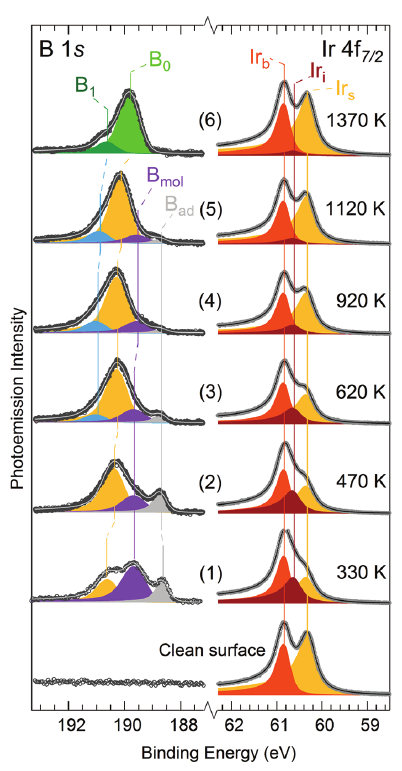
\includegraphics[width=0.9\linewidth]{./images/07571n_fig5.png}
 \caption{\cite{orlando_epitaxial_2012}}
\label{fig:borazine-TPG-on-Ir}
\end{wrapfigure}

Figure \ref{fig:borazine-TPG-on-Ir} shows a typical XPS spectrum of a TPG process with borazine adsorbed on a Iridium surface. At the graphics' bottom one can see the clean Ir surface with no borazine adsorbed (no sign of B1s). There are two contributions in the Ir-peak. While the low energy ($Ir_s$) peak stems from the surface atoms of the subtrate, $Ir_b$ denotes the contribution from the atoms in the bulk. Upon borazine adsorption $(1)$ a broad $B1s$ emerges accompanied with a new contribution in the $Ir$-peak which is a result of borazine-Ir interaction decreasing the intensity of $I_b$ and $I_s$ .

Upon annealing ($(2)$-$(6)$) this peak looses in intensity while the $I_b$ and $I_s$ recover to their initial position. Interesting changes happen to the $B1s$ peak. While at lower temperatures, several peak contributions can be distinguished, denoted as $B_{mol}$ for entire molecules and $B_{ad}$ for molecular fragments. With increasing temperature, $B_{mol}$ decreases for a increase in the $B_0$ peaks. At lower temperature (1), $B_{mol}$ decreases and $B_{ad}$ slightly increases. When exceeding 620K ($\approx \SI{350}{\celsius}$, (3)) a new peak emerges and develops into $B_1$ when increasing temperatures. When temperature is high enough the only peaks left are $B_0$ and $B_1$ - the two contributions of boron atoms stem from boron atoms interact with the Iridium substrate with different strength due to different registry to the substrate.

While usaually borazine is used as precourser different other options exist like B-Trichloroborazine (${ClBNH}_3$) \cite{auwarter_synthesis_2004-1}.
  \section{Surfaces and adlayers}
     \subsection{Crystal facets}
         Crystal orientation and distances: (FIND NICE IMAGES FOR THAT!!)
\begin{table}
\centering
\caption{Interatomic distances for Cu and Ag (both fcc) with respect to different surfaces. $a$ denotes the lattice constant and $\beta$ describes the angle within the (111) unit cell \SI{60}{\degree}}
  \begin{tabular}{ccccc}
& Lattice constant a [\SI{}{\angstrom}] & Nearest neighbours [\SI{}{\angstrom}] & diagonal [\SI{}{\angstrom}] \\ \hline \hline
\multicolumn{2}{c}{fcc(100)} & $\frac{\sqrt{2}a}{2}$ & a \\
  Cu	 	& 3.61	& 2.55 | 2.55 & 3.61 \\
  Ag		& 4.09	& 2.89 | 2.89 & 4.09 \\ \hline 
\multicolumn{2}{c}{fcc(110)} & $\frac{\sqrt{2}a}{2}$ | a & $\sqrt{\frac{3}{2}}a$\\
  Cu	 	& 3.61	& 2.55 | 3.61	& 4.42 \\
  Ag		& 4.09	& 2.89 | 4.09	& 5.00 \\ \hline 
\multicolumn{2}{c}{fcc(111)} & $\frac{\sqrt{2}a}{2} \ <110>$ & $\sqrt{2}a\sin(\frac{\beta}{2})$ | $\sqrt{2}a\cos(\frac{\beta}{2})$\\
  Cu 		& 3.61	& 2.55 | 2.55	& 2.55 | 4.42 \\
  Ag		& 4.09	& 2.89 | 2.89	& 2.89 | 5.01 \\ \hline
 \end{tabular}

\end{table}
 
 ``This surface consists of (111) terraces (three close-packed rows wide) and intrinsic (100) steps, which run parallel to the [011] direction. The close-packed atom rows located at the step edges are characterized by
a nearest-neighbour distance of \SI{2.55}{\angstrom}  for Cu and of \SI{2.89}{\angstrom} for Ag, whereas the intrinsic step
spacing is \SI{6.25}{\angstrom} for Cu and \SI{7.08}{\angstrom} for Ag. The surface symmetry is described by a primitive
rectangular unit cell (cf. Figure 3.1a). The (111) terraces and the microfacets which represent the intrinsic (100) steps are tilted by \SI{19.5}{\degree}, respectively, to macroscopic (211) surface, which can be seen in the side view of the hard-sphere model in the upper panel of Figure 3.1a. The interlayer spacing for this surface is \SI{0.74}{\angstrom} for Cu and \SI{0.83}{\angstrom} for Ag.''

Dense packed rows are for fcc(111) the followgin directions: $<\bar 1 01>$, $<01\bar 1>$, $<1\bar 1 0>$. The diagonals are found in the $<\bar 1 \bar 1 2>$ and $<1\bar 2 1>$ directions.

``The (311) surface consists also of (111) terraces (two close-packed rows wide) and intrinsic (100) steps.''

\begin{table}\label{tab:crystal-prop}
\caption{Crystal porperties from \cite[29ff]{riemann_ionic_2002} and \cite{liu_oxygen_2014}}
\centering
\begin{tabular}{cccc}
			&				& Copper 	 & Silver \\
\multicolumn{2}{c}{Lattice constant}			& \SI{3.61}{\angstrom} & \SI{4.08}{\angstrom} \\
\multicolumn{2}{c}{Nearest neighbour}			& \SI{2.55}{\angstrom} & \SI{2.89}{\angstrom} \\ \hline \\
\multirow{3}{*}{intrinsic step separation}	& (311) & \SI{4.23}{\angstrom} & \SI{4.78}{\angstrom} \\
						& (211) & \SI{6.25}{\angstrom} & \SI{7.07}{\angstrom} \\
						& (221) & \SI{7.66}{\angstrom} & \SI{8.65}{\angstrom} \\
						& (110) & \SI{1.38}{\angstrom} & \\
						& (111) & \SI{1}{\angstrom} & \\
\end{tabular}
\end{table}
Cu(100) has a step height of \SI{1.8}{\angstrom}. See http://dx.doi.org/10.1103/PhysRevB.94.064106
See \cite{riemann_ionic_2002} for another exmaples of vicinal metal surfaces (531),(532),(221),(311),(211).

The surface free energy increases from the (111) surface with increasing angle of the (hkl) surface of interest $$\cos(\phi)=\frac{h+k+l}{\sqrt{3(h^2+k^2+l^2)}}$$ \cite{jian-min_calculation_2004}. Thus, the (111) surface is the one with lowest energy, followed by (110) and (100).

\subsection{Dislocation lines and crystal orientation}
Due to the fact, that dislocastion lines move within the crystal in a defined manner, one can determine the crystals orientation when the orientation of a dislocation is known.
As for FCC crystals the orientation of dislocation lines occures in the {111} plane in $<110>$ direction. Its Burgers vector is $\frac{a}{2}[110]$\cite{_dislocation-theory}.
     \subsection{Surface states}
	In the discussion of surface states, one generally distinguishes between Shockley states[5] and Tamm states,[6] named after the American physicist William Shockley and the Russian physicist Igor Tamm. However there is no real physical distinction between the two terms, only the mathematical approach in describing surface states is different. 

\paragraph{Shockley states - Electron gas approximation} from wikipedia article \\
Historically, surface states that arise as solutions to the Schr�dinger equation
in the framework of the nearly free electron approximation for clean and ideal surfaces, are called Shockley states. Shockley states are thus states that arise due to the change in the electron potential associated solely with the crystal termination. This approach is suited to describe normal metals and some narrow gap semiconductors. Figures 1 and 2 are examples of Shockley states, derived using the nearly free electron approximation.''

\paragraph{Tamm states - Tight binding approximation (LCAO)} from wikipedia article \\
Surface states that are calculated in the framework of a tight-binding model are often called Tamm states. In the tight binding approach, the electronic wave functions are usually expressed as linear combinations of atomic orbitals (LCAO). In contrast to the nearly free electron model used to describe the Shockley states, the Tamm states are suitable to describe also transition metals and wide gap semiconductors.

\paragraph{Extrinsic surface states} from wikipedia article \\
Surface states originating from clean and well ordered surfaces are usually called intrinsic. These states include states originating from reconstructed surfaces, where the two-dimensional translational symmetry gives rise to the band structure in the k space of the surface.

Extrinsic surface states are usually defined as states not originating from a clean and well ordered surface. Surfaces that match the category extrinsic are :
\begin{itemize}
 \item Surfaces with defects, where the translational symmetry of the surface is broken.
 \item Surfaces with adsorbates
 \item Interfaces between solid and liquid phases.
 \item Interfaces between two material such as a semiconductor-oxide or semiconductor-metal interfaces
\end{itemize}
Generally, extrinsic surface states cannot easily be characterized in terms of their chemical, physical or structural properties.

The \index{Kondo effect} \textbf{Kondo effect} also plays a role when looking at scattering of electrons on - in this special case - magnetic imputiries. For further reading one is advised to read \cite{kouwenhoven_revival_2001} and citations within.
     \subsection{Geometric alteration of overlayers -- moire}
	The properties of a moire superstructure are well described in literature and Hermann gives a comprehensive overview in his paper \cite{hermann_periodic_2012}. To sum it up and restrict the information given by him to the cases that occur in this work one can conclude:
\begin{itemize}
 \item A moire is alway present if an overlayer shows a lattice mismatch with respect to the substrate
 \item If lattice constants are equal like in the case of a graphene bilayer, the needed lattice mismatch occures due to a rotation of the two layers.
 \item The moire pattern shows the same Bravais lattice type than the substrate\cite[10]{hermann_periodic_2012} (if the overlayer is isotropically scaled). The Bravais lattice type 
 \item For isotropically scaled overlayers (no distinct stretch direction) one can calculate the scaling factor $$p=\frac{R^{'}_{O1}}{R_{O1}}$$ which gives the size of the overlayer lattice in units of the substrate lattice. 
 \item If moire and lattice are aligned ($\alpha=0$\textdegree) the direction of moire and substrate is aligned.
 \item If the overlayer is isotropically scaled and not rotated, the period of the moire calculates to $$a_{Moire}=\underbrace{\frac{p}{|p-1|}}_{\kappa}a_{substrate}$$
 \item For a scaled and rotated overlayer, the angle between substrate and moire ($\gamma$[rad]) scales with the angle of overlayer and substrate ($\alpha$[rad]) as $$\alpha=(1-p)\gamma$$
 \item For rotated and isotropically scaled overlayers, one can determine the $\alpha$ and $p$ from experimental obervables $\gamma$(moire angle to substrate) and $\kappa$(scaling factor) through relations $$ \tan(\alpha)=\frac{sin(\gamma)}{cos(\gamma)+\kappa}\qquad p=\frac{\kappa}{\sqrt{1+\kappa^2+2\kappa cos(\gamma)}}$$
\end{itemize}


  \section{Used molecules}
    \label{chapter:used-molecules}
The following molecules have been used to conduct experiments. Images show the molecules on a first layer copper crystal background (lattice constant \SI{2.55}{\angstrom}) to elucidate their size. Second and proceeding crystal layers are not shown for better visibility. All images show the molecules on the same substrate area (\SI{2.5}\times\SI{2.5}{\square\nm}). 

All the depicted molecules are modelled in Hyperchem\cite{_hyperchemtm_1111} and calculated for optimized geometry with the AM1+ method. Afterwards their positions are exported and remodelled in blender. Note that this does not change their geometry. It is only for better control of the output (faster and more accurate model building) and for some aesthetic reasons.

Unless stated otherwise the sample was kept at room temperature during dosage.

%%%%%%%%%%%%%%%%%%%%%%%%%%%%%%%%%%%%%%%%%%%%%%%%%%%%%%%%%%%%%%%%%%%%%%%%%%%%%%%%%%%%%%%%%%%
%%%%%%%%%%%%%%%%%%%%%%%%%%%%%%%%%%%nitro-prophines%%%%%%%%%%%%%%%%%%%%%%%%%%%%%%%%%%%%%%%%%
\paragraph{TBP}
\begin{itemize}
 \item Free base nitrophenyl - 5,10,15 Tri [di-[tert-butyl]-phenyl)] porphyrin \textbf{nitro porhin} \\ have 3(2) di-tert-butyl-phenyl groups attached to the macrocycle at the meso-positions of the molecule. The free meso-positions are occupied with nitrophenyl groups. If more than one functional group os prensent, one can destinguish between trans- and cis-configuration, whether the functional groups are opposite or neighbouring. See figure \ref{fig:nitro-trans-cis} for their graphical representation.
 \item In STM this molecules looks almost symmetrical, except the nitro-group which appears dark in STM, making the di-tert-butyl groups the most identifiable parts of the molecule.
 \item The appearence of STM data is correlated to the molecular configuration according to \cite{mishra_current-driven_2015} meaning that the lobes consiting of (3,5-di-tert-butylphenyl) are imaged as bright protrusions, while the functional nitro group is imaged fainter. This holds true for cis- and trans-substituted molecules.

\end{itemize}
Drawings for various functional groups and molecules can be found in \cite{jorgensen_salem_1973}

\begin{itemize}
\item[two-leg cis:] 	5,10-Bis(3,5-di-tert-butylphenyl)-15,20-Bis(Nitrophenyl)porphyrine
\item[two-leg trans:] 	5,15-Bis(3,5-di-tert-butylphenyl)-10,20-Bis(Nitrophenyl)porphyrine
\item[one-leg:] 	5,10,15-Tri(3,5-di-tert-butylphenyl)-20-(Nitrophenyl)porphyrine
\end{itemize}

\begin{figure}[ht]
 \begin{center}
 \subfigure[Single functional group]{
  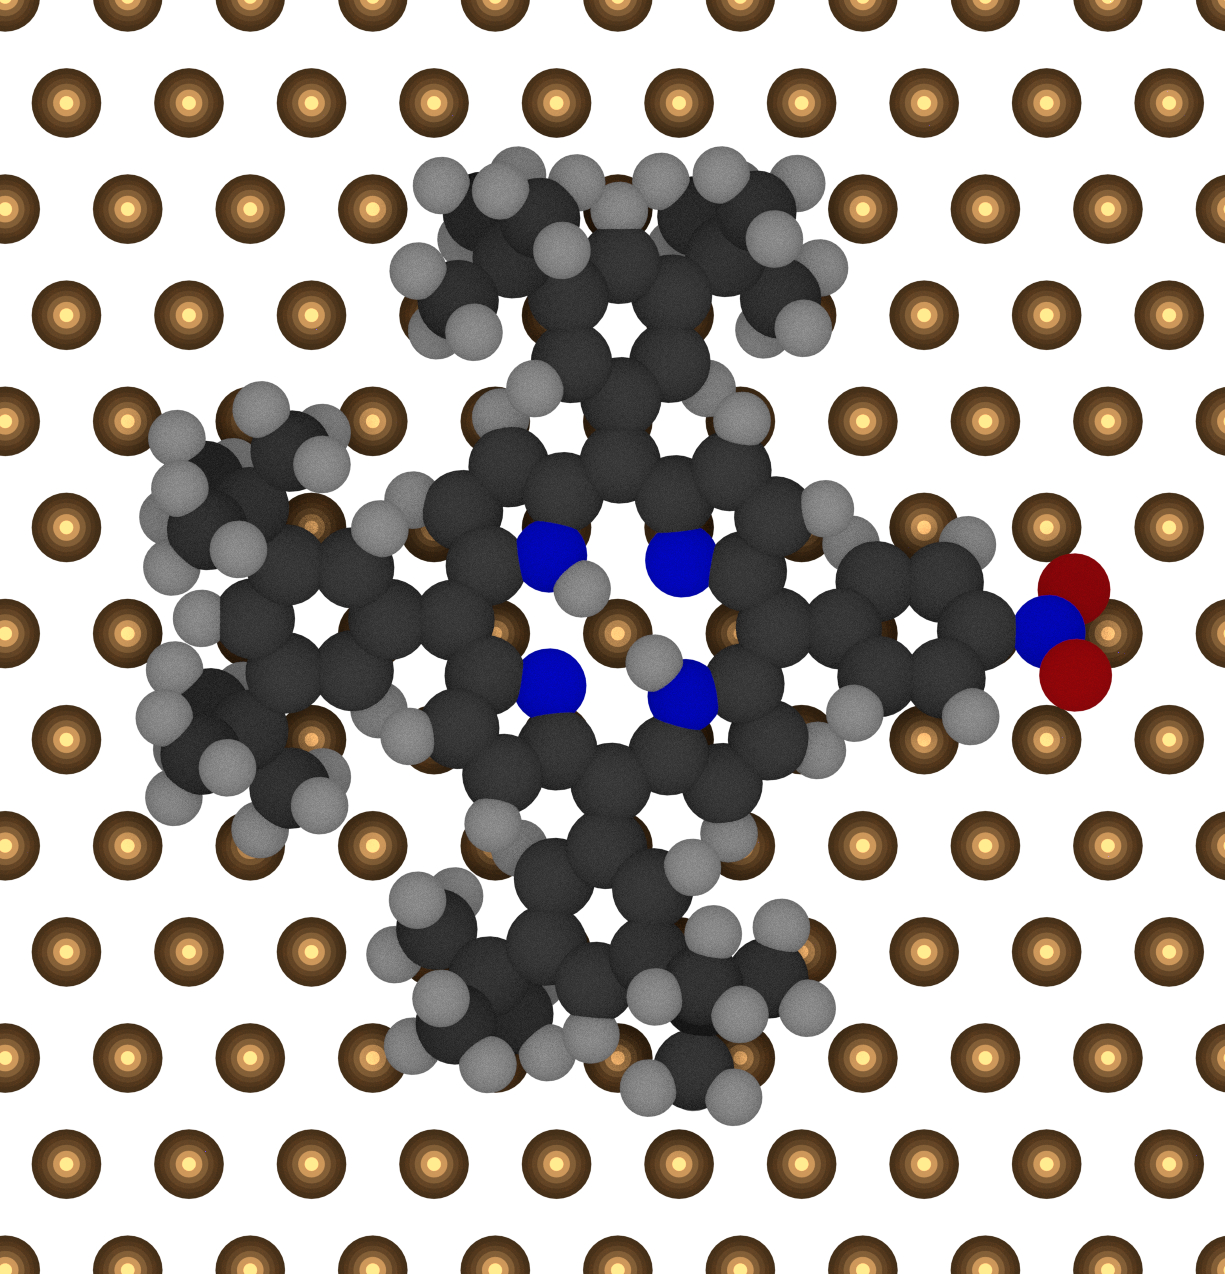
\includegraphics[width=0.3\textwidth]{./images/one-leg-TBP-top.jpg}
 }
 \subfigure[Trans-configuration]{
  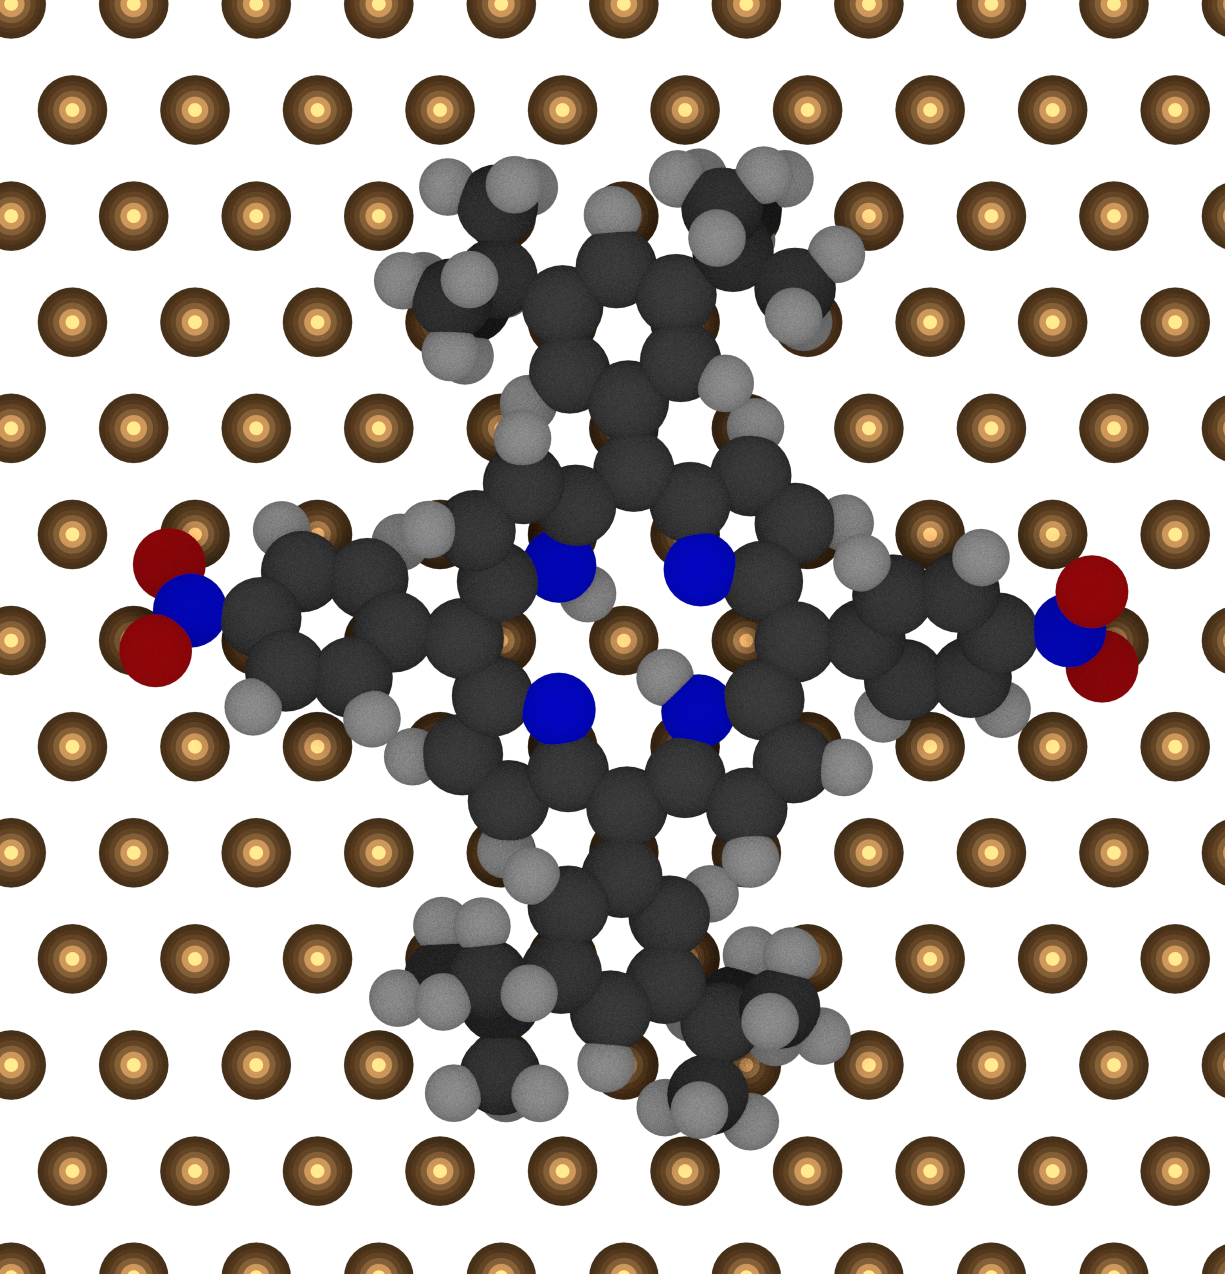
\includegraphics[width=0.3\textwidth]{./images/trans-TBP-top.jpg}
 }
 \subfigure[Cis-configuration]{
  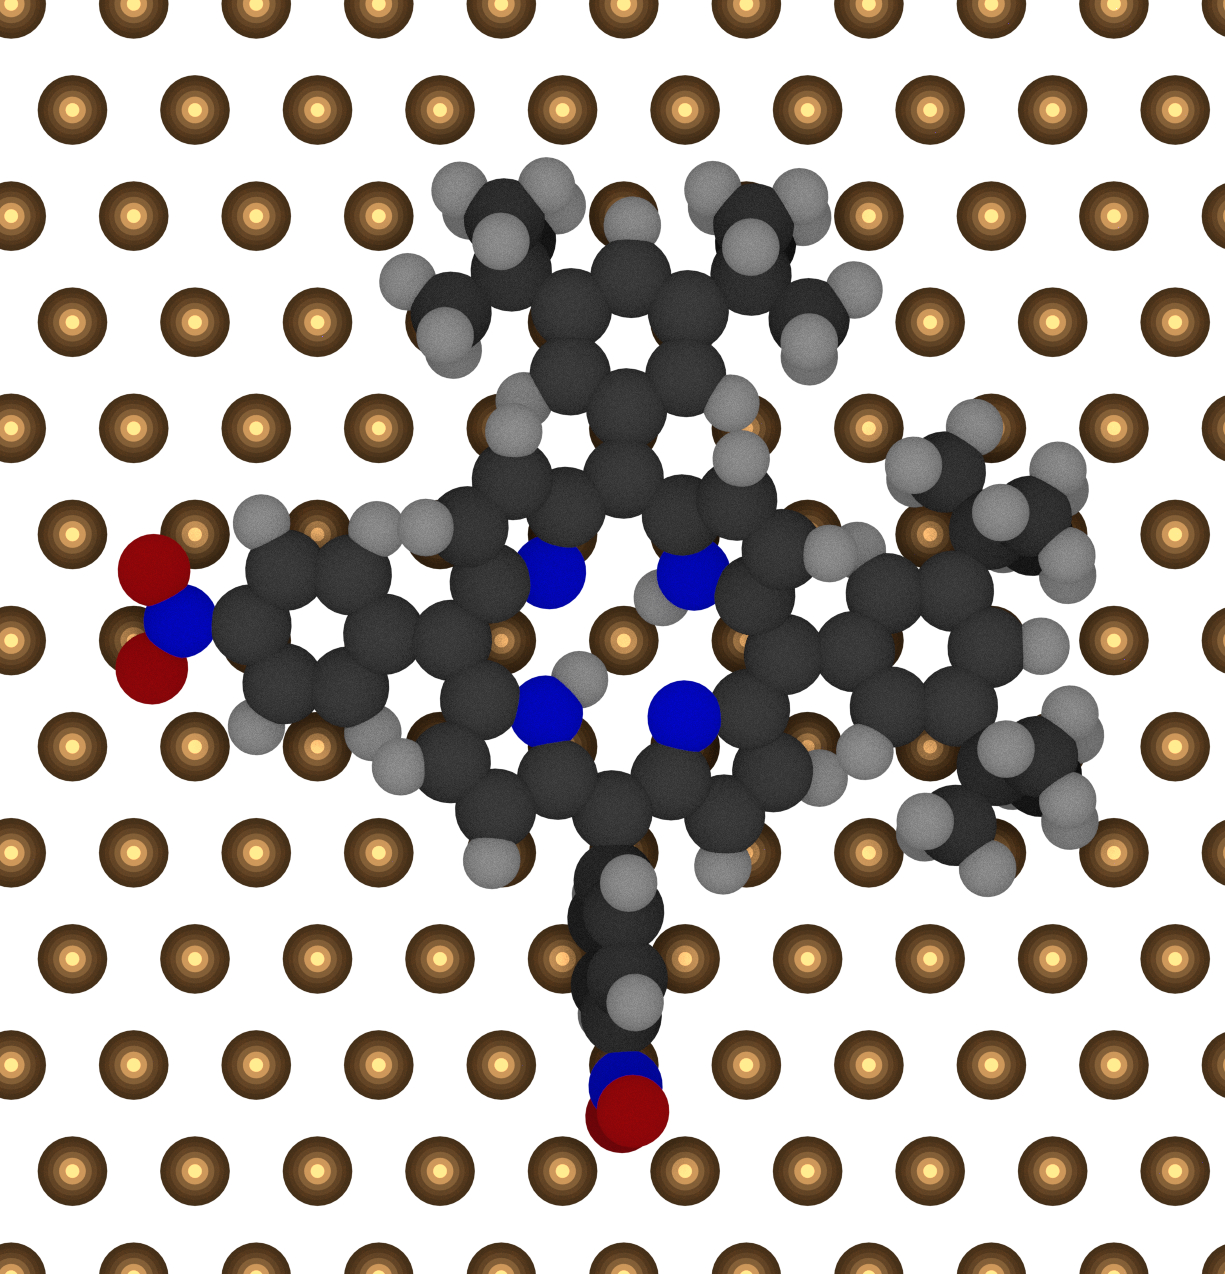
\includegraphics[width=0.3\textwidth]{./images/cis-TBP-top.jpg}
 }
 \end{center}
\caption{Functionalized tert-butyl-phenyl-porphines. Position of the functional nitrophenyl changes and determines its name.}
\label{fig:nitro-trans-cis}
\end{figure}
%%%%%%%%%%%%%%%%%%%%%%%%%%%%%%%%%%%%%%%%%%%%%%%%%%%%%%%%%%%%%%%%%%%%%%%%%%%%%%%%%%%%%%%%%%%
%%%%%%%%%%%%%%%%%%%%%%%%%%%%%%%%%%%	pyrenes   %%%%%%%%%%%%%%%%%%%%%%%%%%%%%%%%%%%%%%%%%
\paragraph{pyrenes}
\begin{itemize}
\item[cis-pyrene:] 1,8-Bis(4-Pyridylethynyl)pyrene
\item[trans-pyrene:] 1,6-Bis(4-Pyridylethynyl)pyrene
\item[tetra-pyrene:] 1,6,8,13-Tetra(4-Pyridylethynyl)pyrene
\end{itemize}

\begin{figure}[ht]
 \begin{center}
 \subfigure[Trans-configuration]{
  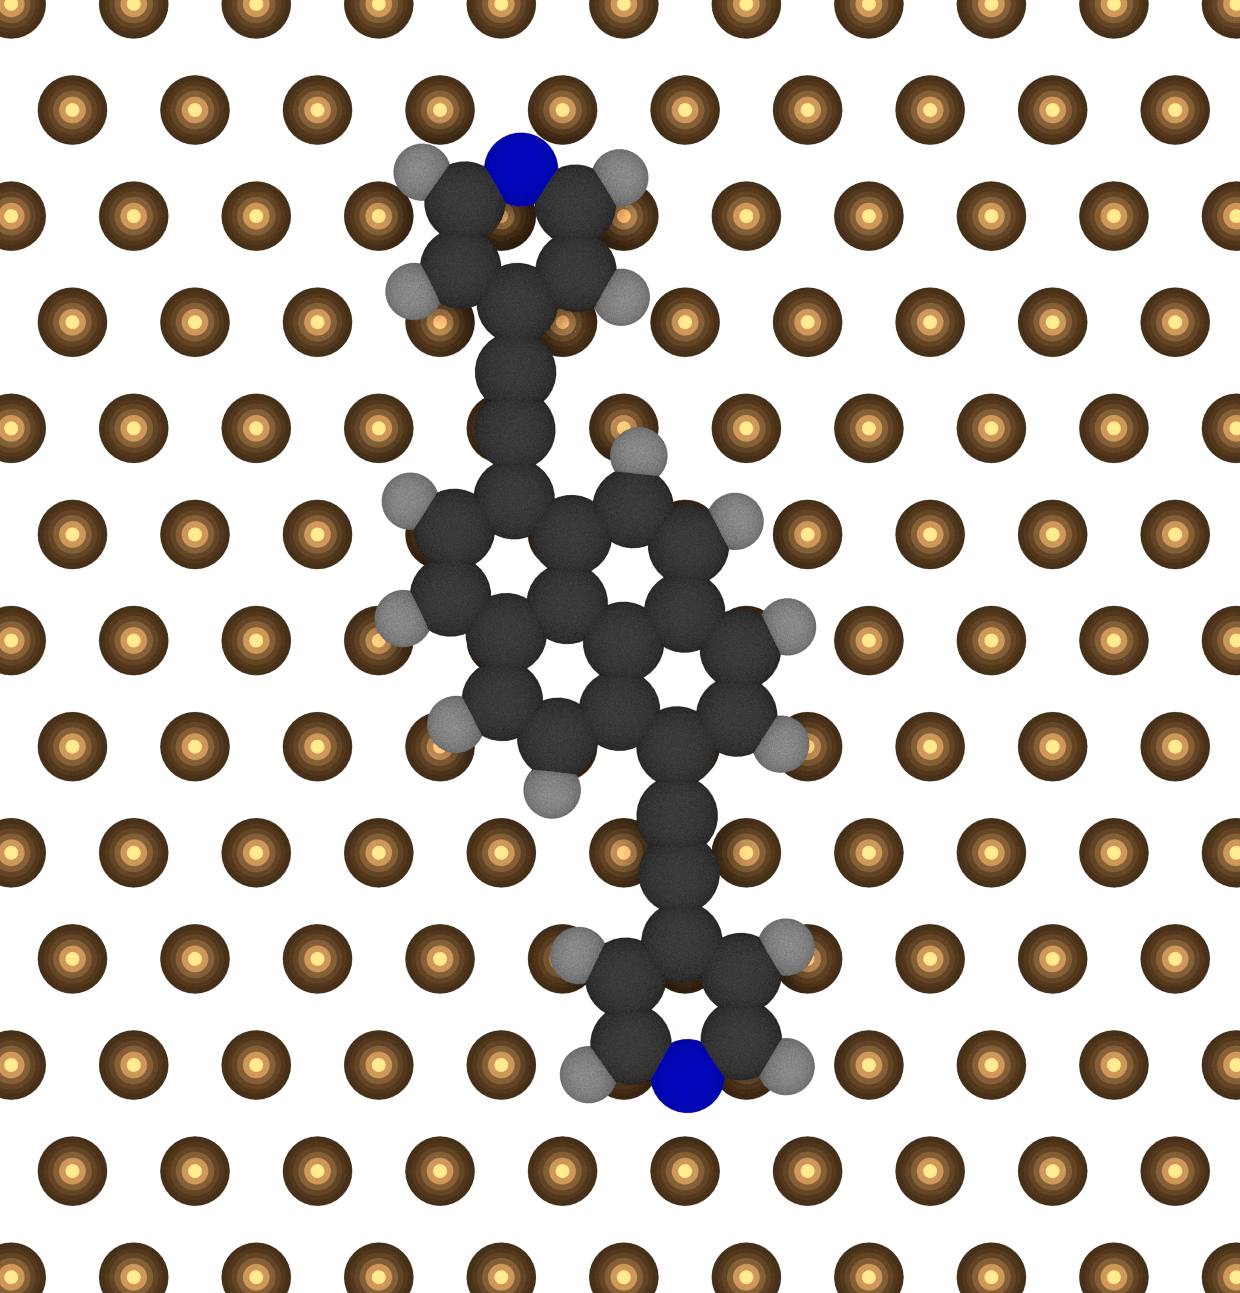
\includegraphics[width=0.3\textwidth]{./images/trans-pyrene-top.jpg}
 }
 \subfigure[Cis-configuration]{
  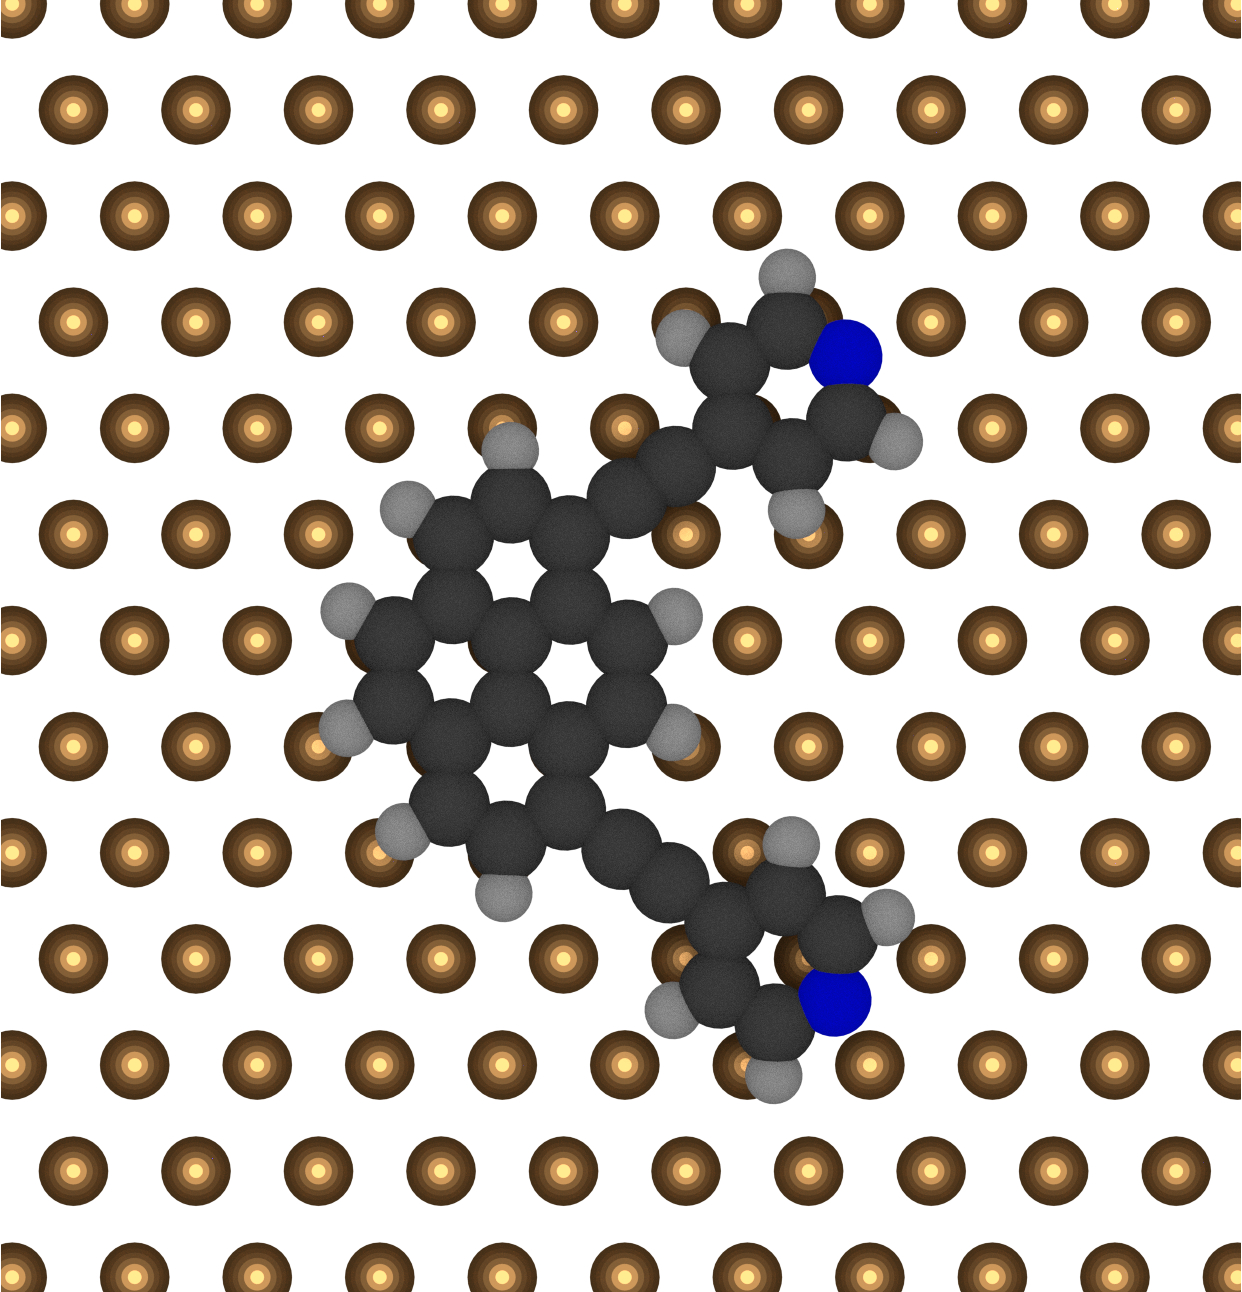
\includegraphics[width=0.3\textwidth]{./images/cis-pyrene-top.jpg}
 }
 \end{center}
\caption{Pyridyl-Pyrene molecules in trans- (a) and cis- (b) configuration}
\end{figure}
%%%%%%%%%%%%%%%%%%%%%%%%%%%%%%%%%%%%%%%%%%%%%%%%%%%%%%%%%%%%%%%%%%%%%%%%%%%%%%%%%%%%%%%%%%%
%%%%%%%%%%%%%%%%%%%%%%%%%%%%%%%%%%%	TPCN      %%%%%%%%%%%%%%%%%%%%%%%%%%%%%%%%%%%%%%%%%
\paragraph{TPCN}
TPCN can be evaporated with an OMBE. Temperatures used are typically \SI{490}{\celsius}, evaporation time depends on the intended coverage. 
\begin{itemize}
 \item [TPCN:] Tetra[(4-cyanophenyl)-phen-4-yl] porphyrin has four arms attached to the meso-positions of the macrocycle. Each is build up from two chained phenyl rings with one end attached to the macrocycle and the other one attached to a C-N end group.
\end{itemize}

\begin{figure}[ht]
 \begin{center}
  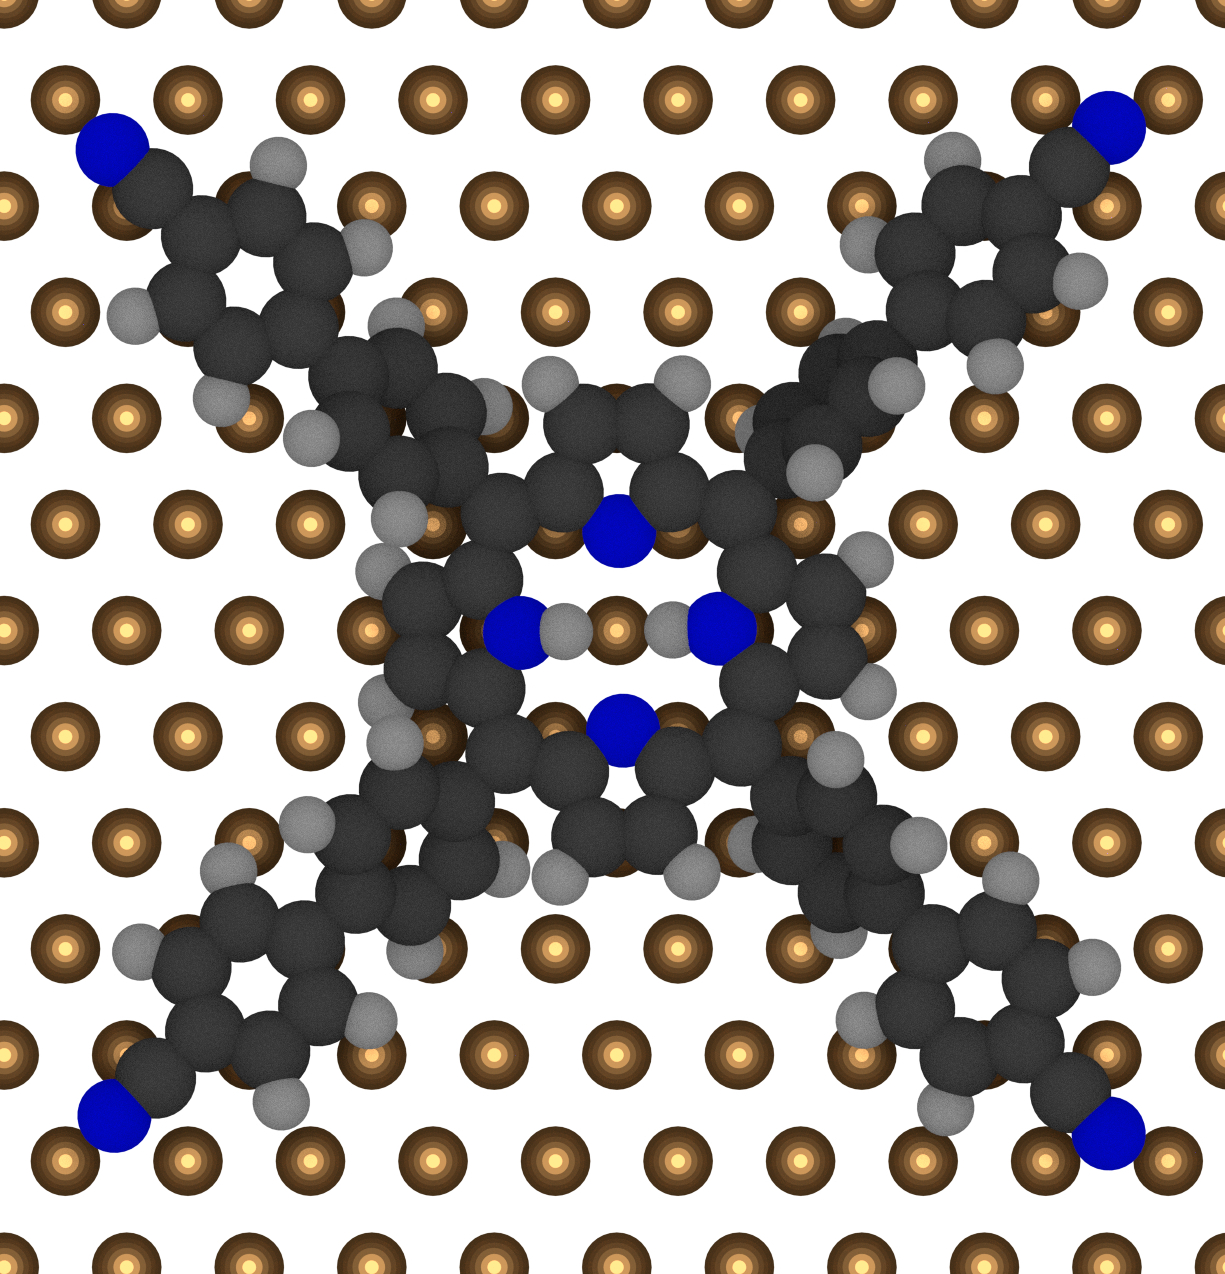
\includegraphics[width=0.3\textwidth]{./images/TPCN-top.jpg}
 \end{center}
\caption{TPCN}
\end{figure}
%%%%%%%%%%%%%%%%%%%%%%%%%%%%%%%%%%%%%%%%%%%%%%%%%%%%%%%%%%%%%%%%%%%%%%%%%%%%%%%%%%%%%%%%%%%
\begin{table}
 \centering
 \caption{Evaporation and degas temperatures used for different molecules.}
 \begin{tabular}{ccrc}
Name			& Configuration & Degas [\SI{}{\degreeCelsius}]	& Evaporate [\SI{}{\degreeCelsius}]	\\ \hline \hline 
TPCN			& ---		& ---		& 490		\\ \hline 
\multirow{3}{*}{TBP}	&single		& \SI{4}{\hour} @ \SI{200}{\degreeCelsius}& 390	\\
			&cis		& ---		& \SI{400}{\degreeCelsius}\\
			&trans		& \SI{4}{\hour} @ \SI{200}{\degreeCelsius} + \SI{1}{\hour} @ \SI{270}{\degreeCelsius}&\SI{370}{\degreeCelsius}\\ \hline 
\multirow{4}{*}{pyrene} & \multirow{3}{*}{cis}		& \SI{2}{\hour} @ \SI{180}{\degreeCelsius}&	\multirow{3}{*}{250}	\\
&&+ \SI{1}{\hour} @ \SI{200}{\degreeCelsius} + \SI{10}{\minute} @ \SI{235}{\degreeCelsius} 	&\\
&&+ \SI{1}{\hour} @ \SI{220}{\degreeCelsius}&\\ 
			&trans		& \SI{1}{\hour} @ \SI{230}{\degreeCelsius}		&\SI{265}{\degreeCelsius}		\\ \hline
\multirow{3}{*}{DCDB} & \multirow{3}{*}{---} & 1h @ \SIrange{100}{150}{\degreeCelsius}& \multirow{3}{*}{\SIrange{220}{240}{\degreeCelsius}}\\
&&+\SI{10}{\minute} @ \SI{170}{\degreeCelsius} + \SI{25}{\minute} @ \SI{200}{\degreeCelsius} & \\
&&+ \SI{40}{\minute} @ \SI{220}{\degreeCelsius}&\\
 \end{tabular}
\label{tab:molecule-temperatures}
\end{table}


%%%%%%%%%%%%%%%%%%%%%%%%%%%%%%%%%%%%%%%%%%%%%%%%%%%%%%%%%%%%%%%%%%%%%%%%%%%%%%%%%%%%%%%%%%%
%%%%%%%%%%%%%%%%%%%%%%%%%%%%%%%%%%%	helicenes %%%%%%%%%%%%%%%%%%%%%%%%%%%%%%%%%%%%%%%%%
\paragraph{helicenes}
\begin{itemize}
% \item[[7]-CN-helicene:] 2,16-Bis(cyano)-helicene
\item[Dicyano-Dibenzo-[5]helicene:] 7,8-Bis(cyano)-Dibenzo-helicene
\end{itemize}

% \begin{figure}[ht]
%  \centering
%  \subfigure[Top view]{
%   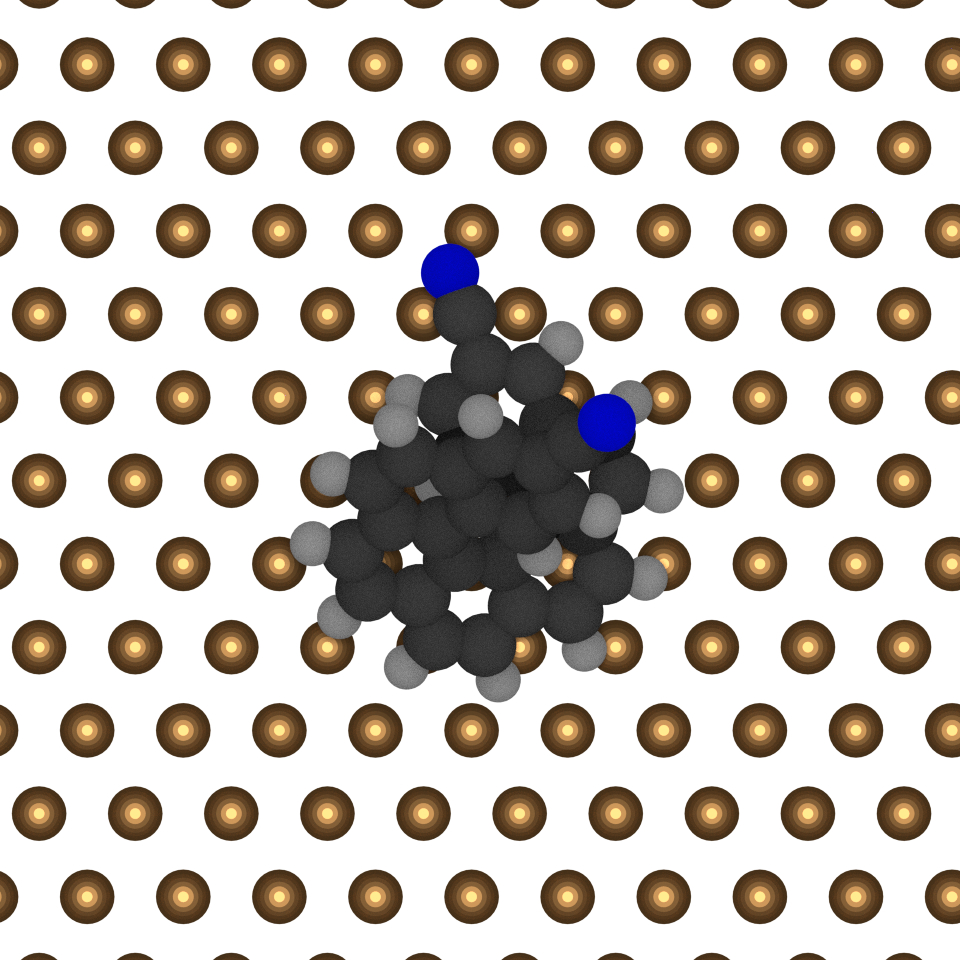
\includegraphics[width=0.3\textwidth]{./images/7-helicene-CN-AM1-top.jpg}
%   }
%  \subfigure[Sideview]{
%   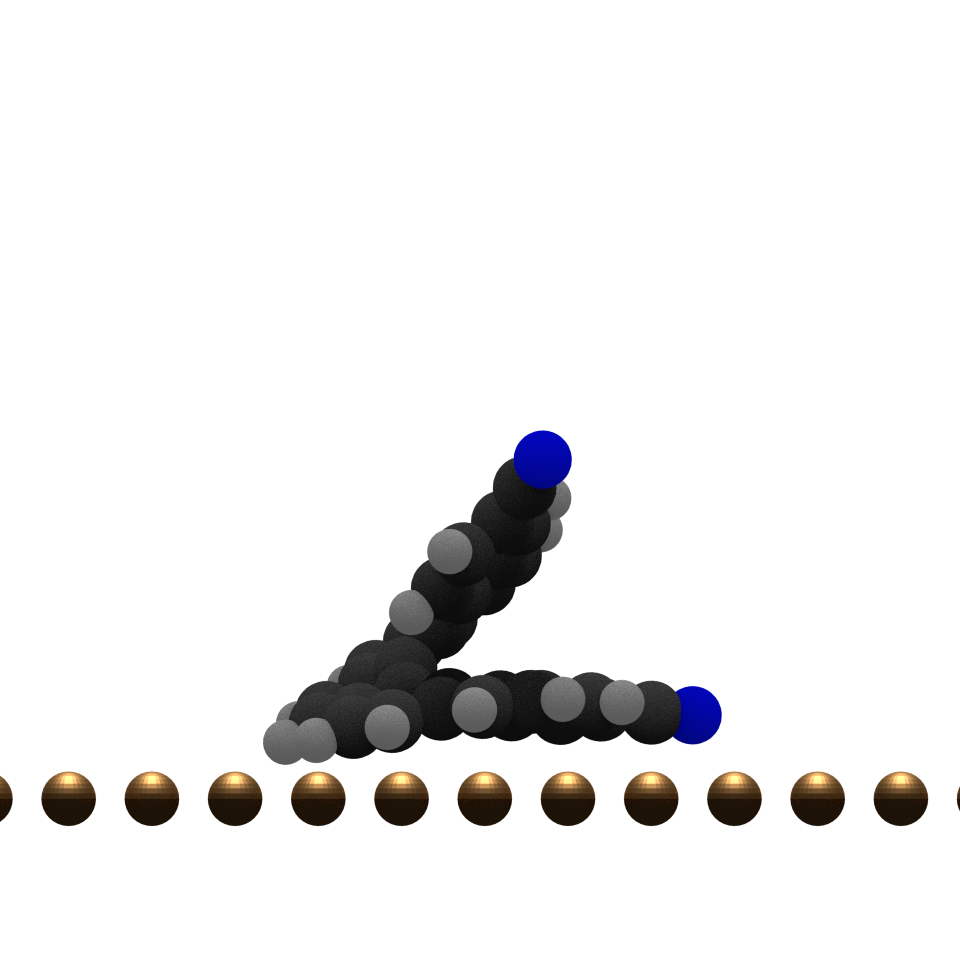
\includegraphics[width=0.3\textwidth]{./images/7-helicene-CN-AM1-side.jpg}
%   }
% \caption{[7]-CN-helicene on copper surface. a) Top view, b) side view}
% \end{figure}

\begin{figure}[ht]
 \centering
 \subfigure[Top view]{
  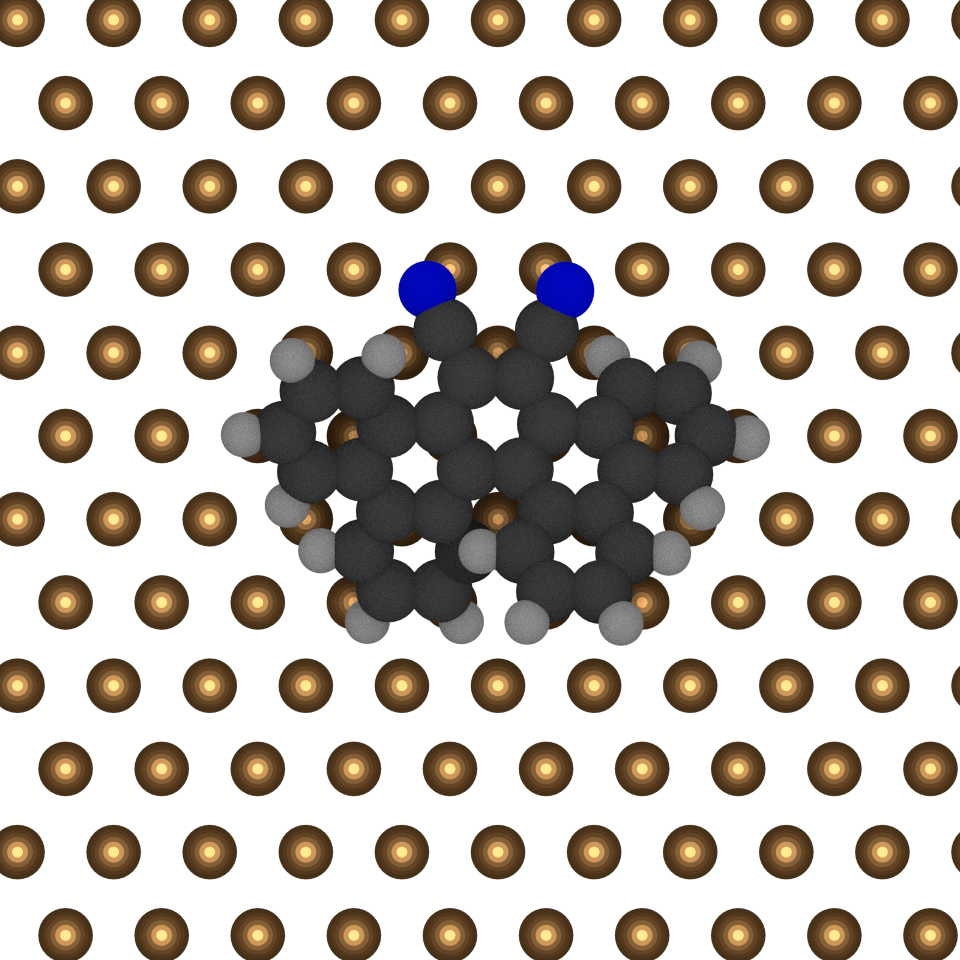
\includegraphics[width=0.3\textwidth]{./images/DCDB-AM1-top.png}
  }
 \subfigure[Sideview]{
  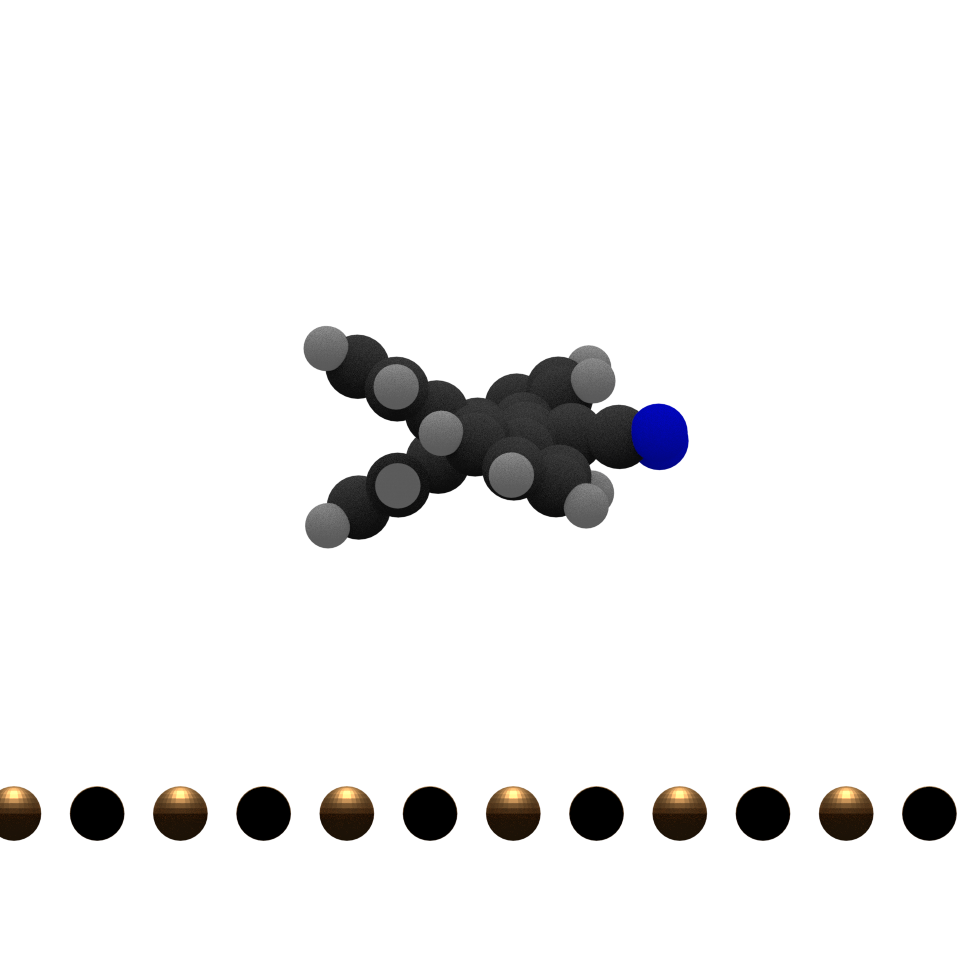
\includegraphics[width=0.3\textwidth]{./images/DCDB-AM1-side.png}
  }
\caption{DCDB on copper surface. a) Top view, b) side view}
\end{figure}

\paragraph{How to determine molecules' distance}
To determine the distance between molecules, one has to carefuly choose the points of interest. As a problem of STM imaging the contour of the molecules sometimes appears as more or less fuzzy shape. There is no sharp edge that one could take as start or end point of the profile. Therefore the center of the molecule is often used as reference point to measure the distance between two molecules (compare fig. \ref{fig:distance-molecules}). As the molecule has a square footprint, one can use the center in one direction (along profile 2/3) to determine the center in the other direction (profile 1). As one can see the three profiles match leading to a consistent center of the dimer. This is also shown as depression in profile 1. 

\begin{figure}[!ht]
\centering
\subfigure[Molecule with chosen profiles (1-3) indicated as white lines.]{
        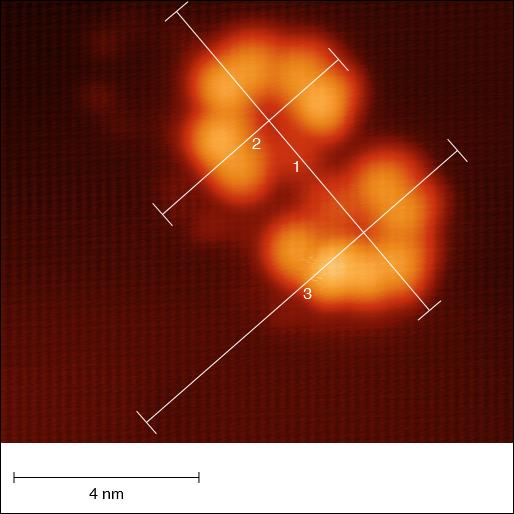
\includegraphics[width=0.45\textwidth]{./images/F150612-163956-dimer-loose.jpg}
}
\subfigure[Profiles 1-3 indicated in a).  Local minima in profile 2/3 indicate central positions in profile 1.]{
	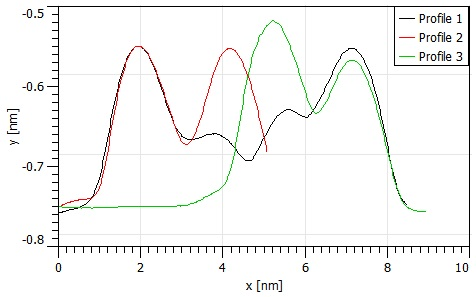
\includegraphics[width=0.45\textwidth]{./images/F150612-163956-profile-dimer-loose.jpg}
}
\caption{Sketch of how to determine the distance between two molecules. As the molecule is square (with the exception of one direction, one can determine the center of the molecule by comparing two 90 degree rotated profiles. Profile 1 goes through the symmetry axis, while profile 2 and 3 intersect profile 1 at the center. As the profile 2 and 3 look the same when starting at the buthyl groups, one can use the depression in profile 2 and 3 to determine the center of the molecule in profile 1.}
\label{fig:distance-molecules}
\end{figure}
\printbibliography

%%%%%%%%%%%%%%%%%%%%%%%%%%%%%%%%%%%%%%%%%%%%%
\chapter{Epitaxial hexagonal boron nitride on copper foils}
\section{Pre-treatment of Cu-foils}
  \subsection{Electropolishing copper foils}
  Growing high quality adlayers on polycrystalline copper foils requires a smooth surface. As-ordered Cu foils exhibit a root-mean-square (rms) surface roughness of about \SI{218}{\nm}\cite{bin_zhang_low-temperature_2012}. Striations - a fabrication remnant due to the cold rolled foils - are observed on the surface\cite{kim_synthesis_2012-1}. Also some manufacturers apply a thin layer of chromium oxide for corrosion protection\cite{bin_zhang_low-temperature_2012}. A common procedure to reduce the roughness of a material is to elctrochemical polish the surface.

A comprehensive overview of \index{electrochemical polishing} electrochemical polishing of Cu surfaces with different etchants can be found in \cite{jinshan_electrochemical_2004}. The following gives a short introduction in chemical polishing:

\paragraph{solution of anode atoms in aqueous cell medium}
Electrons and atoms at the solid surface have higher energy states. Thus some of the atoms on the metal surface may lose electrons to form ions. These ions may also recombine with electrons and become atoms at another moment. Depending on the electronic structures, some metals (such as sodium) are easier than others (such as platinum) to ionize. Copper is relatively stable. Still, some of the surface atoms may be expected to ionize at a moment. The ionization process may be promoted when the metal is in touch with aqueous solution because: 
\begin{itemize}
 \item Metal ions can not move in the metal electrode but can move through the solution, producing electric current in solution with an applied potential
 \item Electrons can move fieely in metal solid (electric current in a metal) but can not survive in solution and will quickly recombine with positive ions
 \item Water dipoles and negative ions in solution may drag the surface metal ions into the solution
\end{itemize}

\paragraph{chemical reaction}\index{electrochemical polishing!chemical reaction}
``The electrode connected to the positive pole of the power supply is called anode. And the one connected to the negative pole of the power supply is called cathode. When the applied voltage is high enough, electrons in the anode may be pumped out and the metal atoms on the anode surahce will be oxidized (e.g., $Cu - 2e = Cut^{2+}$) and dissolved into the electrolyte solution. Under electrical field, the positive ions (cations) move towards cathode and negative ions (anions) move towards anode. The cations may get electrons and be reduced to neutral atoms (e.g., $Cu^{2-} + 2e = Cu$) again at the cathode surface. Therefore, charge transfer between the two electrodes is carried out via the ion drift in the electrolyte and electron conduction in metal wire. When the working electrode is set to be anode, dissolution is processed at certain potential. Likewise, when the working electrode is set to be cathode, it can result in deposition. For electropolishing of copper, the copper part to be polished is set to be anode while the cathode can be any conductive material (e.g., copper).

The critical potential at which the oxidation / reduction starts to occur is related to the standard redox potential for a specific anode material. The redox potential $E_O$ is a measure (in volts) of the affinity of a substance for electrons - its electronegativity - compared with hydrogen (which is set at 0). Substances more strongly electronegative (i.e., capable of oxidizing or accepting electrons) than hydrogen have positive redox potentials (e.g., $Cu/CU^{2+}$: $E_O = \SI{0.34}{\volt}$). Substances less electronegative (i.e., capable of reducing or giving up electrons) than hydrogen have negative redox potentials (e.g., $Cr^{3+}/Cr^{2+}$: $E_O = \SI{-1.07}{\volt}$)\cite{jinshan_electrochemical_2004}

\paragraph{Removed mass from working electrode}
``The current flow of every two electrons results in one copper atom dissolved on the anode and deposited on the cathode. Since $\SI{1}{\ampere}= \SI{1}{\coulomb \second}$, the charge of one electron $e = \SI{1.60218E16}{\coulomb}$, so the number of electrons (per second) in 1 A current is $N_e = \frac{I}{e}$; the number of copper atoms being oxidized or reduced $N_a= \frac{1}{2} N_e= \frac{I}{2e}$, the number of moles $N_m = \frac{N_a}{N_A} = \frac{I}{2eN_A}= \frac{I}{2F}$ where Avogadro's number $N_A = \SI{6.02214E23}{\per \mole}$. The weight of $N_m$ mole copper $W = N_m M = \frac{IM}{2 F}$ where M is the molecular weight of copper. Thats a volume, $V = W / d =\frac{IM}{2 F d}$ where d is the density of copper. Thus a current I produces a dissolution/deposition rate in thickness (\SI{}{\centi\meter \per \second}) \begin{equation} R_d=\frac{M}{2 FdA}I \label{dissolution-rate}\end{equation}
where A is the area of the electrode surface.
\cite[34]{jinshan_electrochemical_2004}

\paragraph{Voltage-current-characteristic or polarization curve}
\begin{itemize}
 \item[-]On a polycrystalline metal surface there are sites, such as defects and grain boundaries, where atoms are at higher energy states. In addition, due to arbitrary crystal orientation, there are different crystalline planes with different energy states of atoms on the electrode surface. Therefore, atoms at all these different sites and planes have different standard redox potential $E_O$, and as a result, have different dissolution rate according to eq. \ref{dissolution-rate}. Such an anodic dissolution will not lead to polishing. Instead, a crystallographic etching is produced (reference [9, 33-35] within \cite{jinshan_electrochemical_2004}). This is true at lower current (or applied potential). This refers to the "etching" regime in figure \ref{oxygen-pitting} with $U<\SI{1.5}{\volt}$.
 \item[-]The plateau where the current remains almost constant with increasing voltage is referred to as "polishing plateau". Overall, the values of iL and EL of the limiting current plateau and the shape of a polarization curve depends on electrolyte solution, anode material, disk rotating speed, solution circulation, temperature, and the distance between anode and cathode.
Of all the factors, electrolyte is the most important one determining the polarization curve.
 \item[-]With continuing increase of applied potential, other reactions than Cu oxidation and reduction may occur and contribute to the increasing current. These reactions produce $H_2$ and $O_2$ bubbles, which occur at or reach the anode surface.
\end{itemize}

\paragraph{gas bubbling}
Gas (oxygen or hydrogen) bubbles may block $Cu^{2+}$ ion transport and therefore terminate the electrochemical dissolution process on the area inside the bubbles. However, the residual solution on the surface area inside the bubbles may react with Cu atom and result in chemical etching. Depending on the chemical property of the electrolyte solution and the value of current density at which the electrochemical dissolution is occurring, the etching speed can be higher than the rate of electrochemical dissolution. In this case, pits will be produced on the anode and produce a rough surface. If etching does not occur inside the bubbles, or if its speed is slower than that of electrochemical dissolution process, the area inside the bubbles will remain and appears as protruding particles after the electrochemical dissolution process. In either case, a rough surface is produced. Approaches to reduce the effect of oxygen bubbling are done by alterning the etching solution with different additives.

\begin{figure}[!h]
\centering
  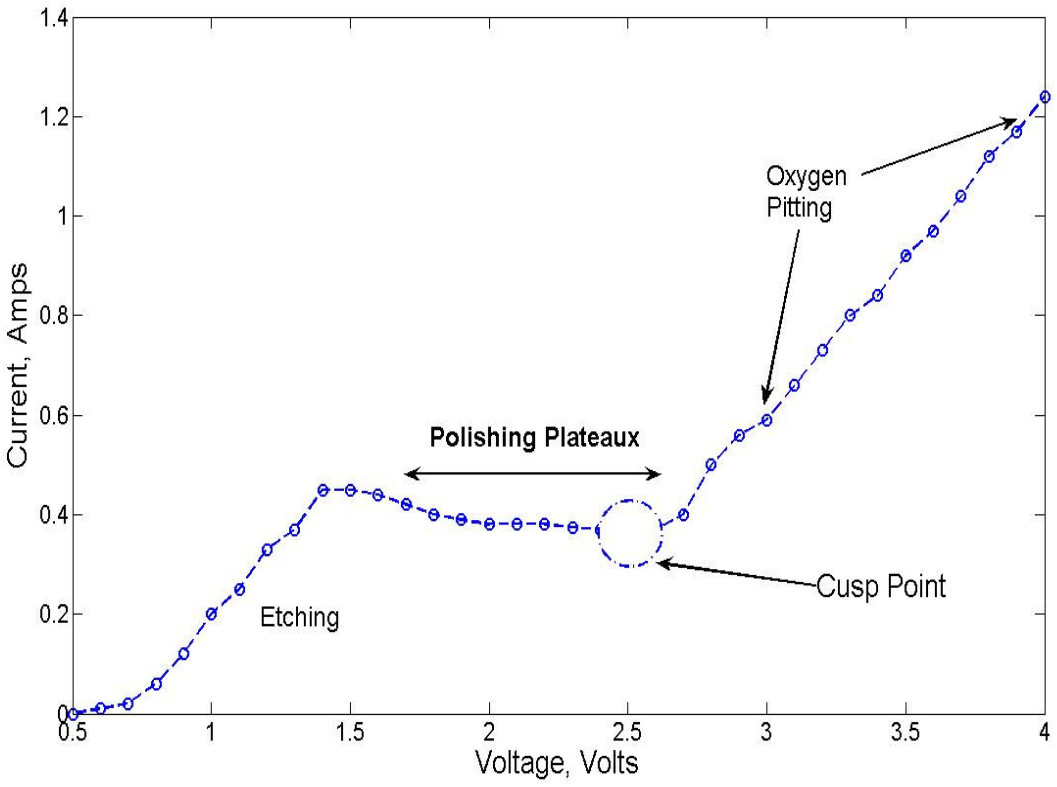
\includegraphics[width=\textwidth]{./images/oxygen-pitting}
\caption{Image reproduced from \cite[3]{stables_report_2008}}
\label{oxygen-pitting}
\end{figure}

\paragraph{experimental things in \cite{jinshan_electrochemical_2004}}
\begin{itemize}
 \item[-]The distance between working and counter electrodes was about 15 mm. All experiments were carried out in a 200 mL glass container at room temperature. 100 mL electrolyte solution was used for each experiment.
 \item[-]Adding EG into phosphoric acid solutions decreases limiting current. The more EG added the lower the limiting current. This is true for both undiluted and diluted (with water) phosphoric acid solution. Dilyuting phosphoric acid - EG solutions with water (25\%, curve 2 in Fig. 3-10) increases limiting current. Further diluting phosphoric acid - EG solutions with water (5O\%, curve 3 in Fig. 3-10) decreases limiting current. Limiting current plateau disappears at solution "12.5\% phosphoric acid + 37.5\% EG + 50\% water.
\end{itemize}
The etching process relies on the fact that the current density (and thus the etching rate) is higher in protruding regions of the copper foil (Ohmic leveling).  As a result the surface of the copper foil will be smoothened \cite{luo_effect_2011}. Compare with migration smoothing and diffusion smoothing\cite{jinshan_electrochemical_2004}.

%%%%%%%%%%%%%%%%%%%%%%%%%%%%%%%%%%%%%%%%%%%%%%%%%%%%%%%%%%%%%%%
%%% ################## minpage for table ##################
\begin{table}[!h]
\centering
\caption{Used chemicals for the etching process}
\begin{tabular}{lll}
 Linear formular & Common name & Fully systematic additive name \\ \hline \hline
$CH_3CH_2OH$   & Ethanol &  Ethanol \\
$H_3PO_4$ & (ortho-)Phosphoric acid & Trihydroxidooxidophosphorus  \\
$NH_2CONH_2$ & Urea & Carbonyldiamide \\
$(CH_3)_2CHOH$  & Isopropanol &  2-Propanol \\
$CH_C(OH)[PO(OH)_2]_2$& HEDP, Etidronic acid &  1-Hydroxyethane-1,1,-diphosphonic acid \\
$[H(OCH_2CH_2)]_nOH$ & (P)EG & (Poly-)Ethylene Glycol\\
%$H_2PO_4^{-1}$ & Dihydrogenphosphate & Dihydroxidooxidophosphorus(1-)  \\
%$HPO_4^{-2}$ & Hydrogenphosphate & Hydroxidooxidophosphorus(2-)  \\
%$[PO_4]^{-3}$ & Phosphate & Tetraoxidophorsphate(3-)  \\ \hline
\end{tabular}
\label{tab:small-molecules}
\end{table}
%%% ################## minpage for table ##################
\begin{figure}[!h]
 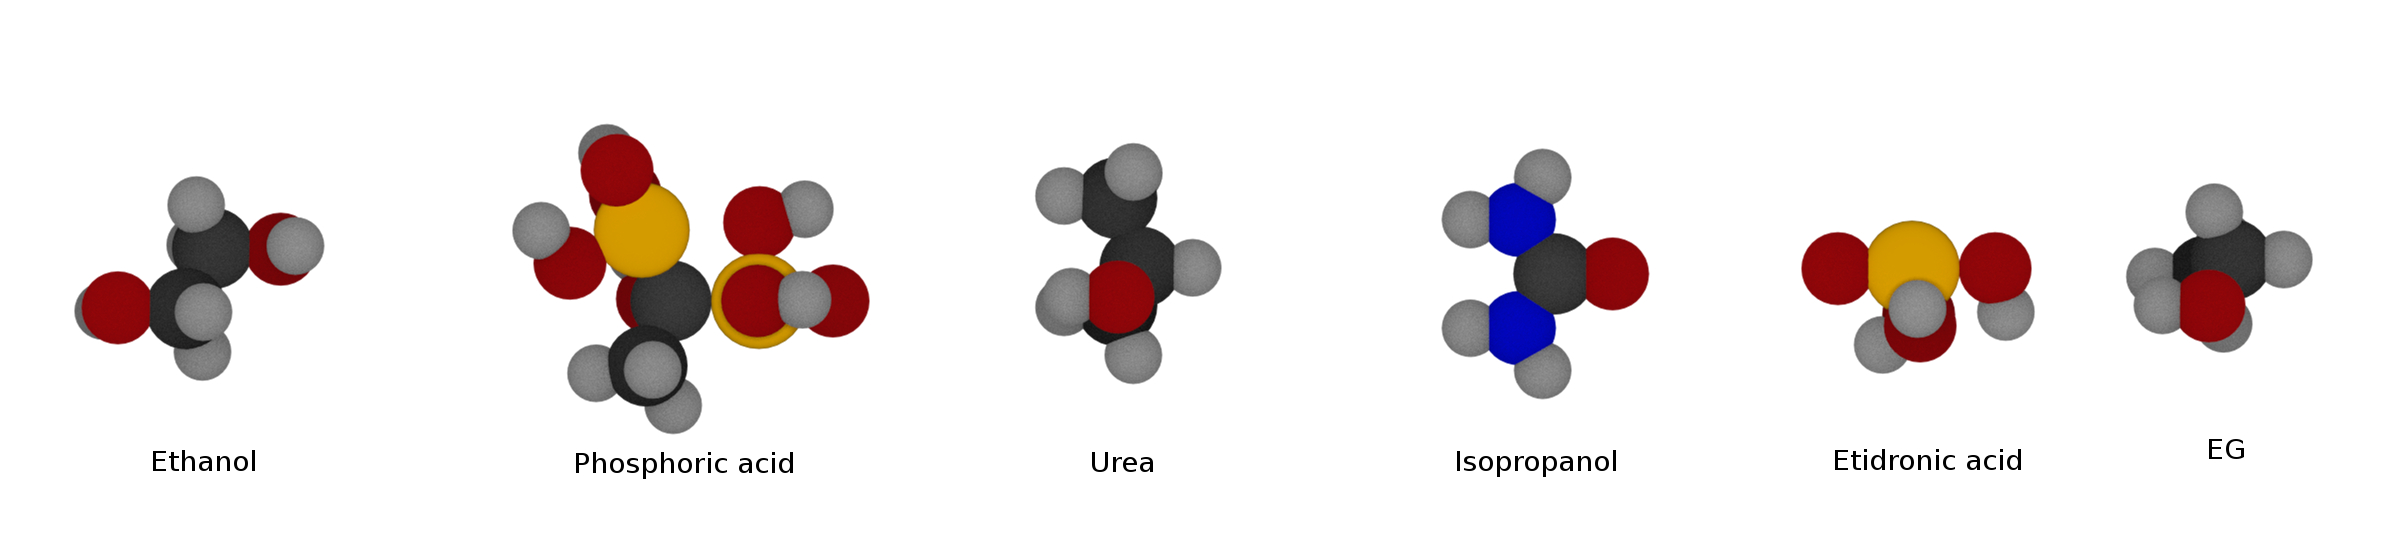
\includegraphics[angle=0,width=\textwidth]{./images/small-molecules-leabelled.jpg}
 \caption{Molecules from table \ref{tab:small-molecules}, in order from top to bottom (left to right).}
\end{figure}

%%%%%%%%%%%%%%%%%%%%%%%% molecules in structure formulas %%%%%%%%%%%%%%%%%%%%%%%% 
% \begin{figure}[h!]
% \centering
% \subfigure[Structure of HEDP(CAS number is 2809-21-4\cite{_hedp_2014}). Image taken from \cite{_hedp_wiki_2014}]{
% 	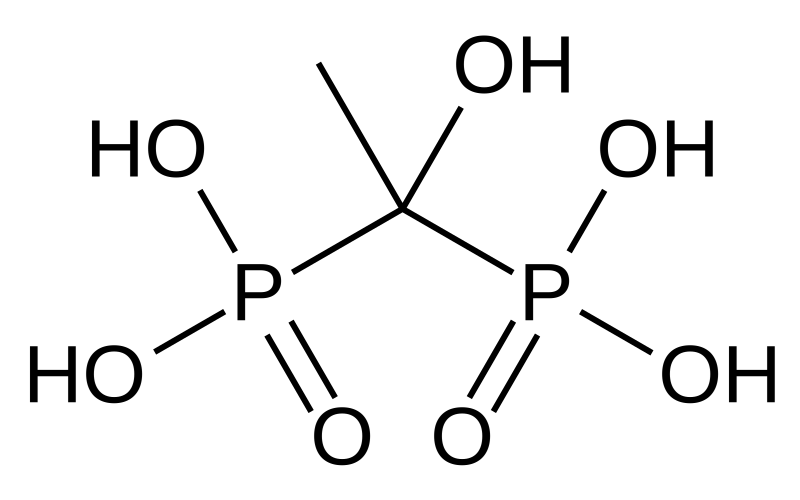
\includegraphics[width=0.45\textwidth]{./images/Etidronic_acid}
% }
% \subfigure[Structure of phosphoric acid(CAS number is 7664-38-2). Modified from \cite{_phosphoric-acid-2d-dimensions.png_2014}]{
% 	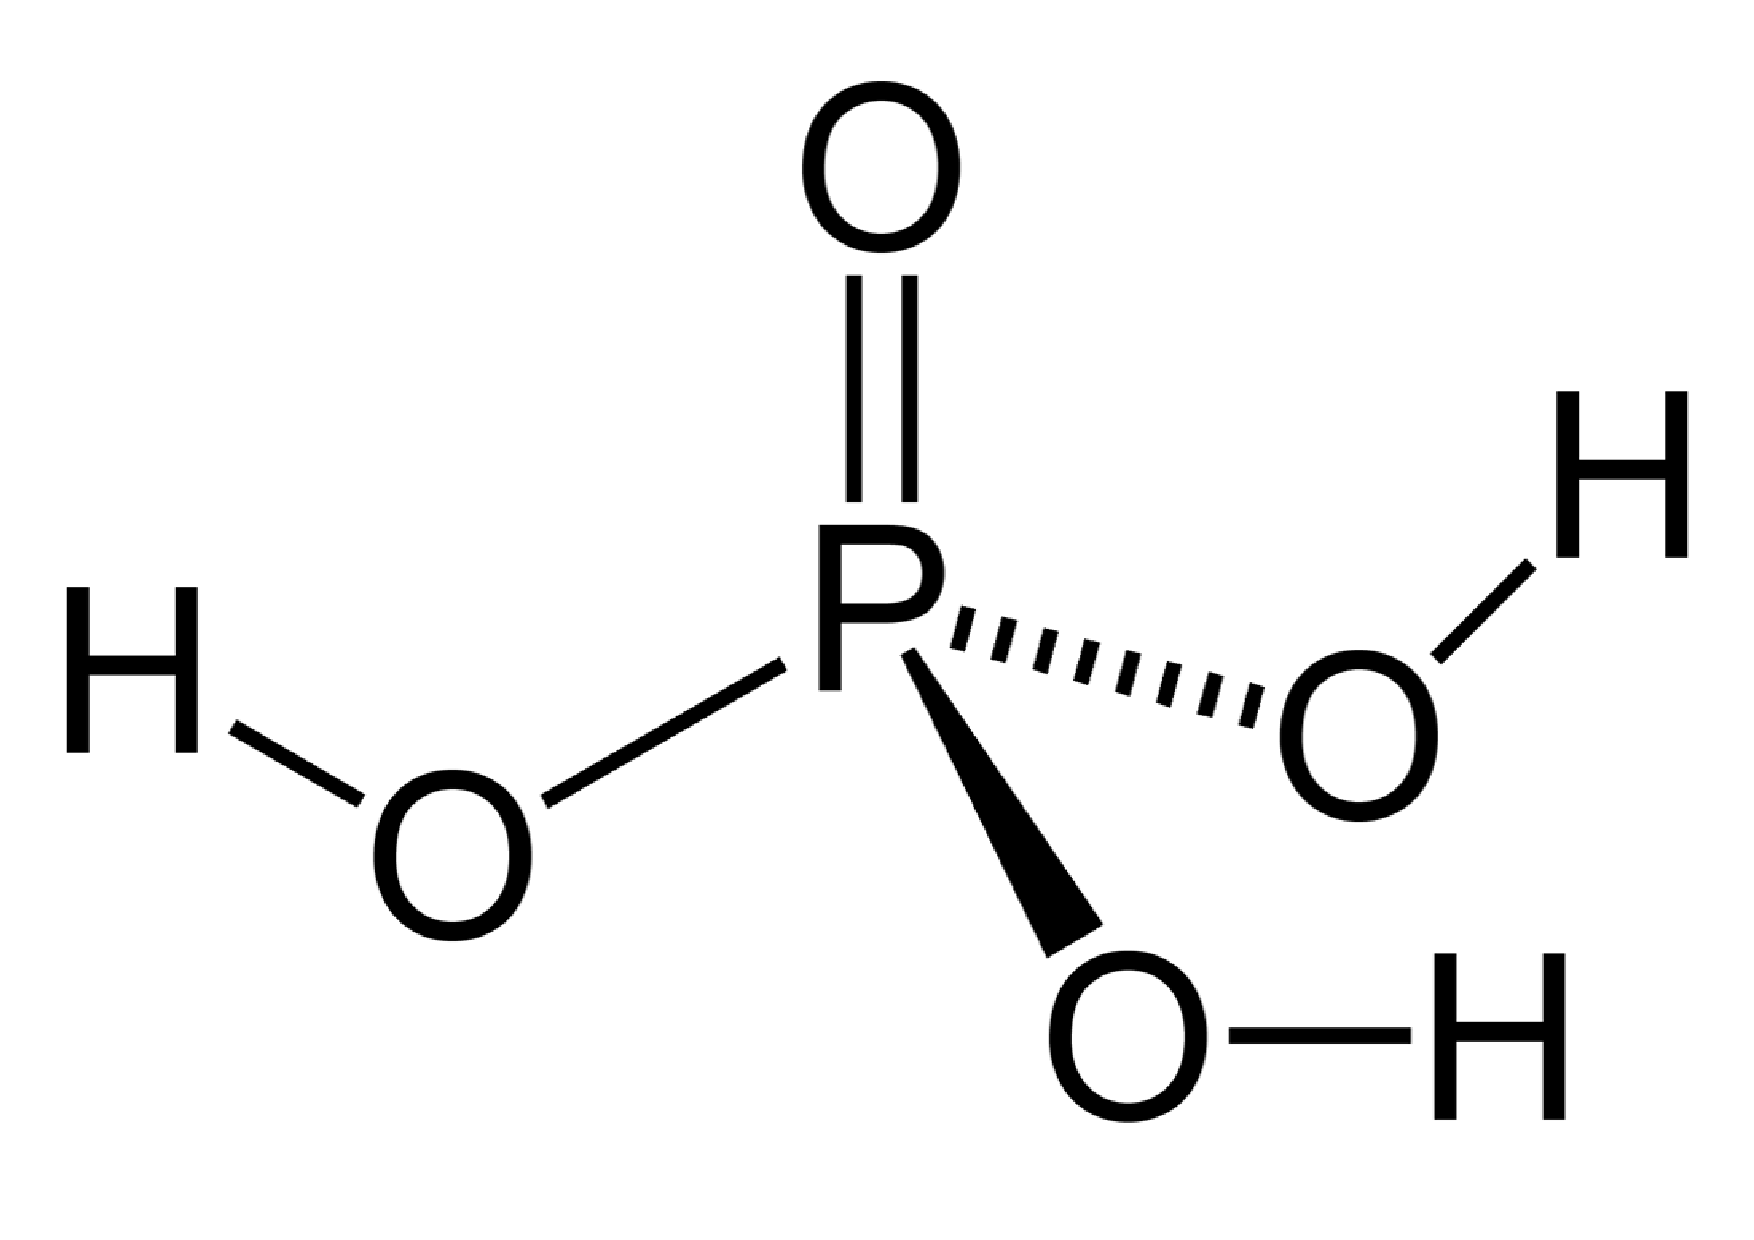
\includegraphics[width=0.45\textwidth]{./images/Phosphoric-acid-2D-dimensions}
% }
% \caption{Different phosphoric acids}
% \end{figure}
% 
% \begin{figure}[h!]
% \centering
% \subfigure[Structure of 2-Propanol (CAS number 67-63-0). Image taken from \cite{_isopropyl_2014}]{
% 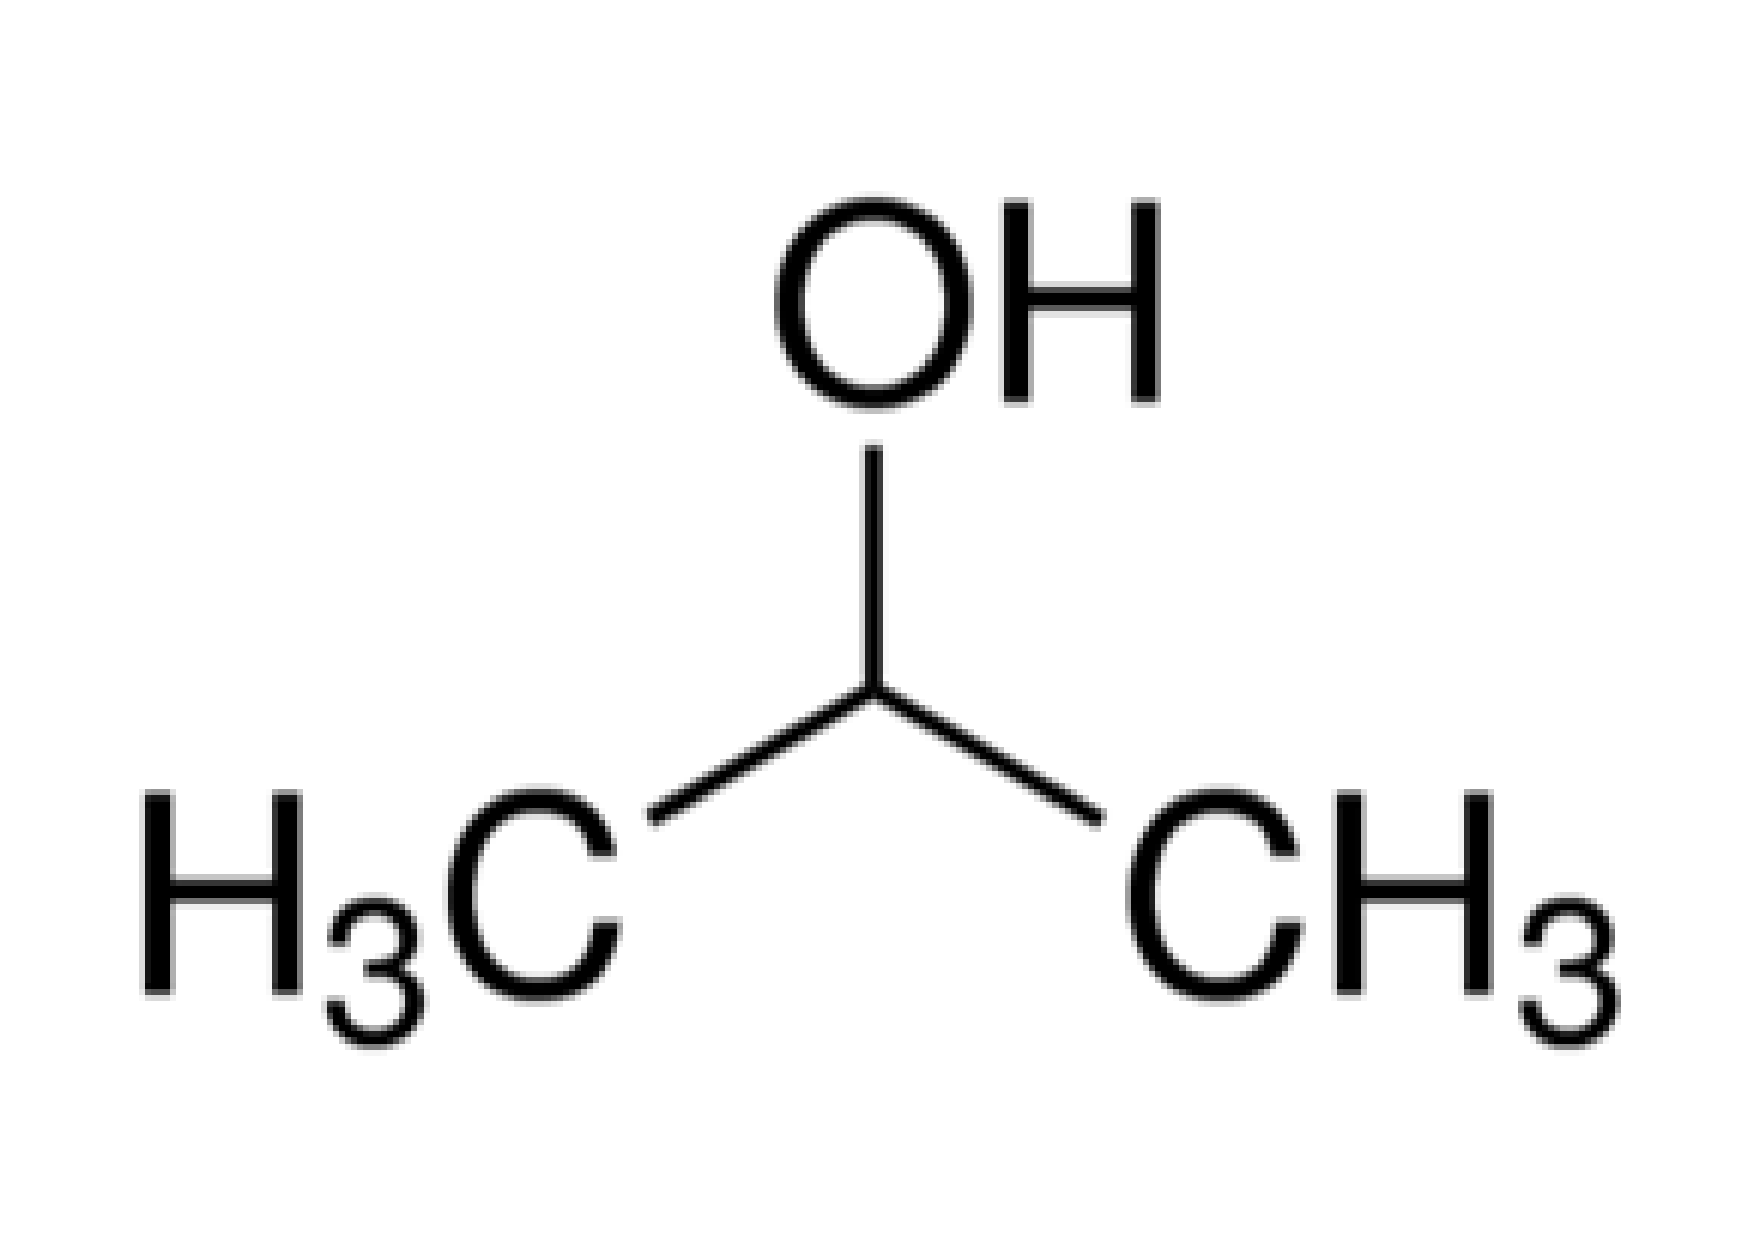
\includegraphics[width=0.45\textwidth]{./images/2-Propanol}
% 	}
% \subfigure[Structure of Ethanol (CAS number 64-17-5). Image taken from \cite{_64-17-5_2014}]{
% 	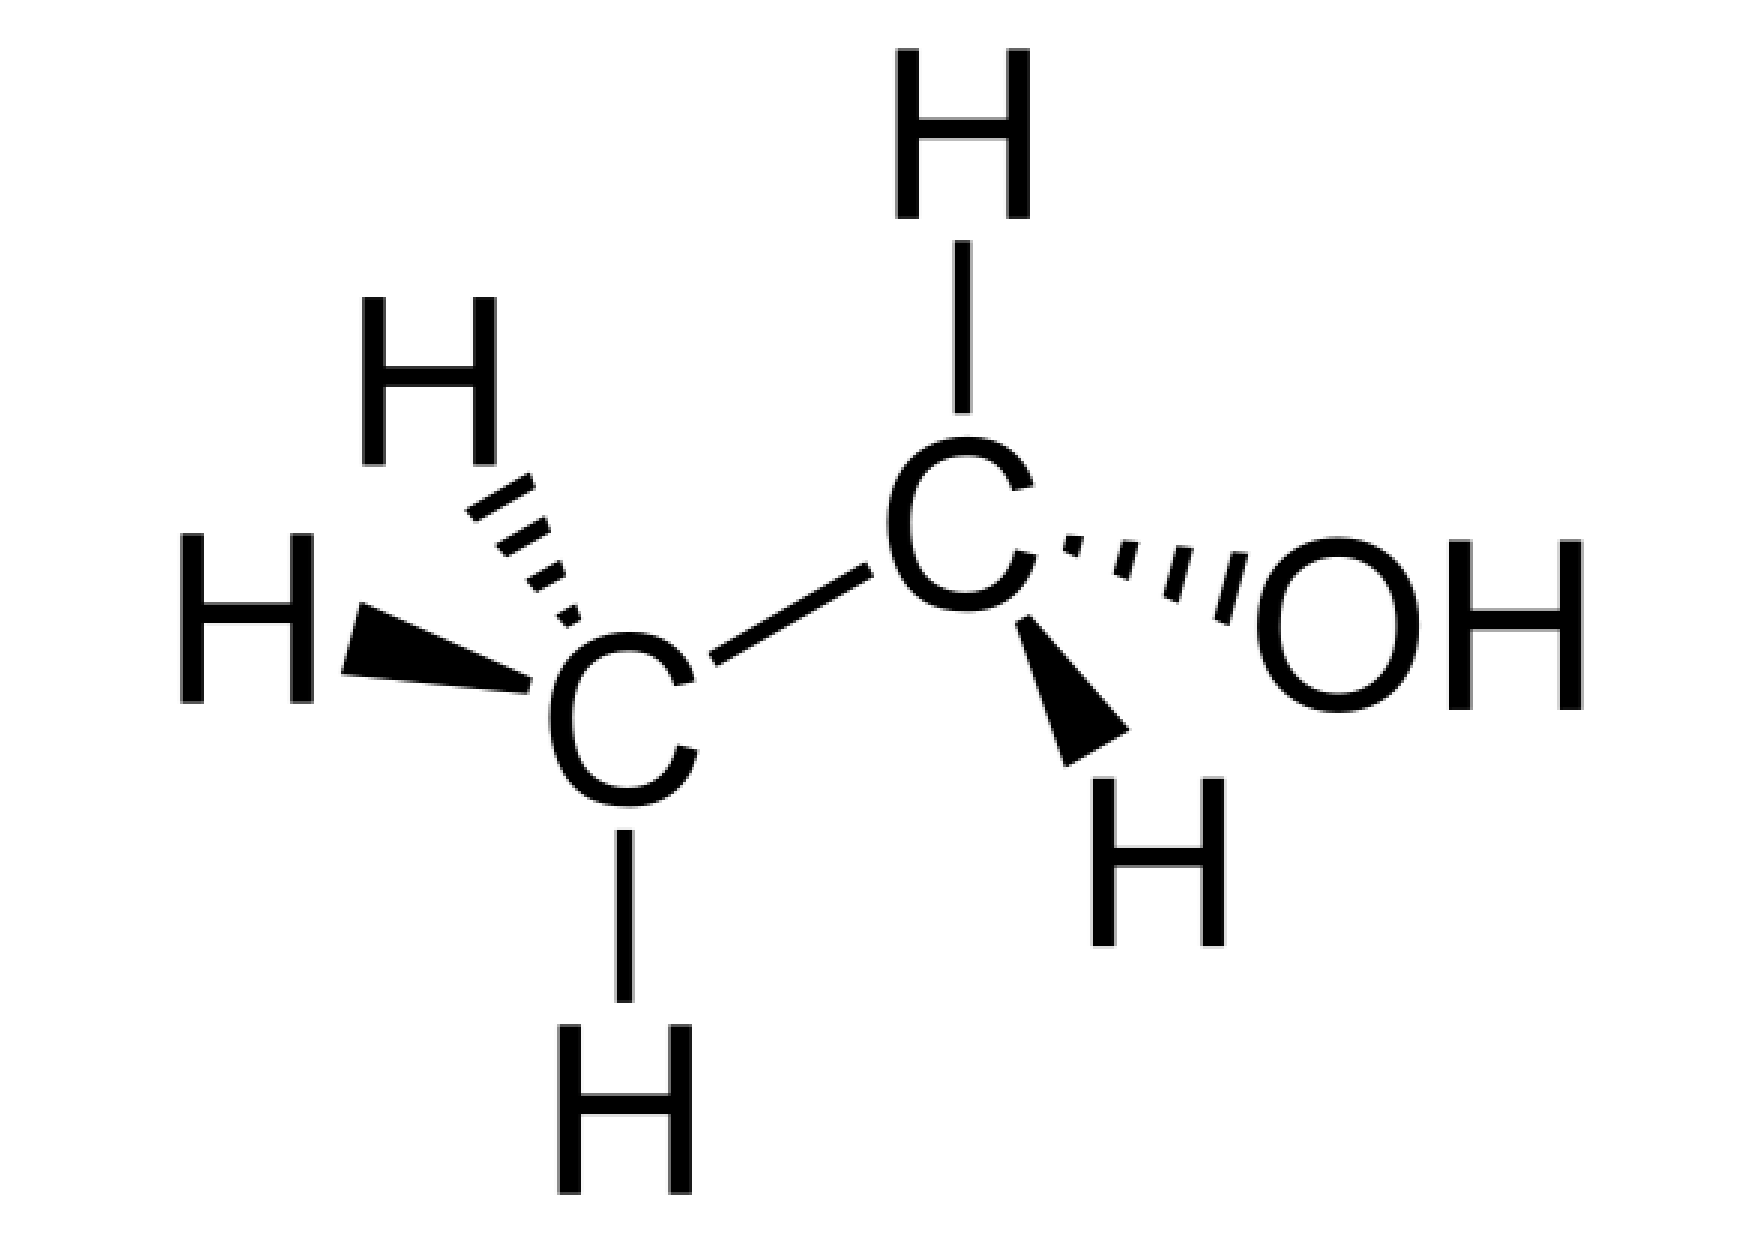
\includegraphics[width=0.45\textwidth]{./images/Ethanol}
% 	}
% \caption{Different alcohols}
% \end{figure}
% 
% \begin{figure}
% \centering
%   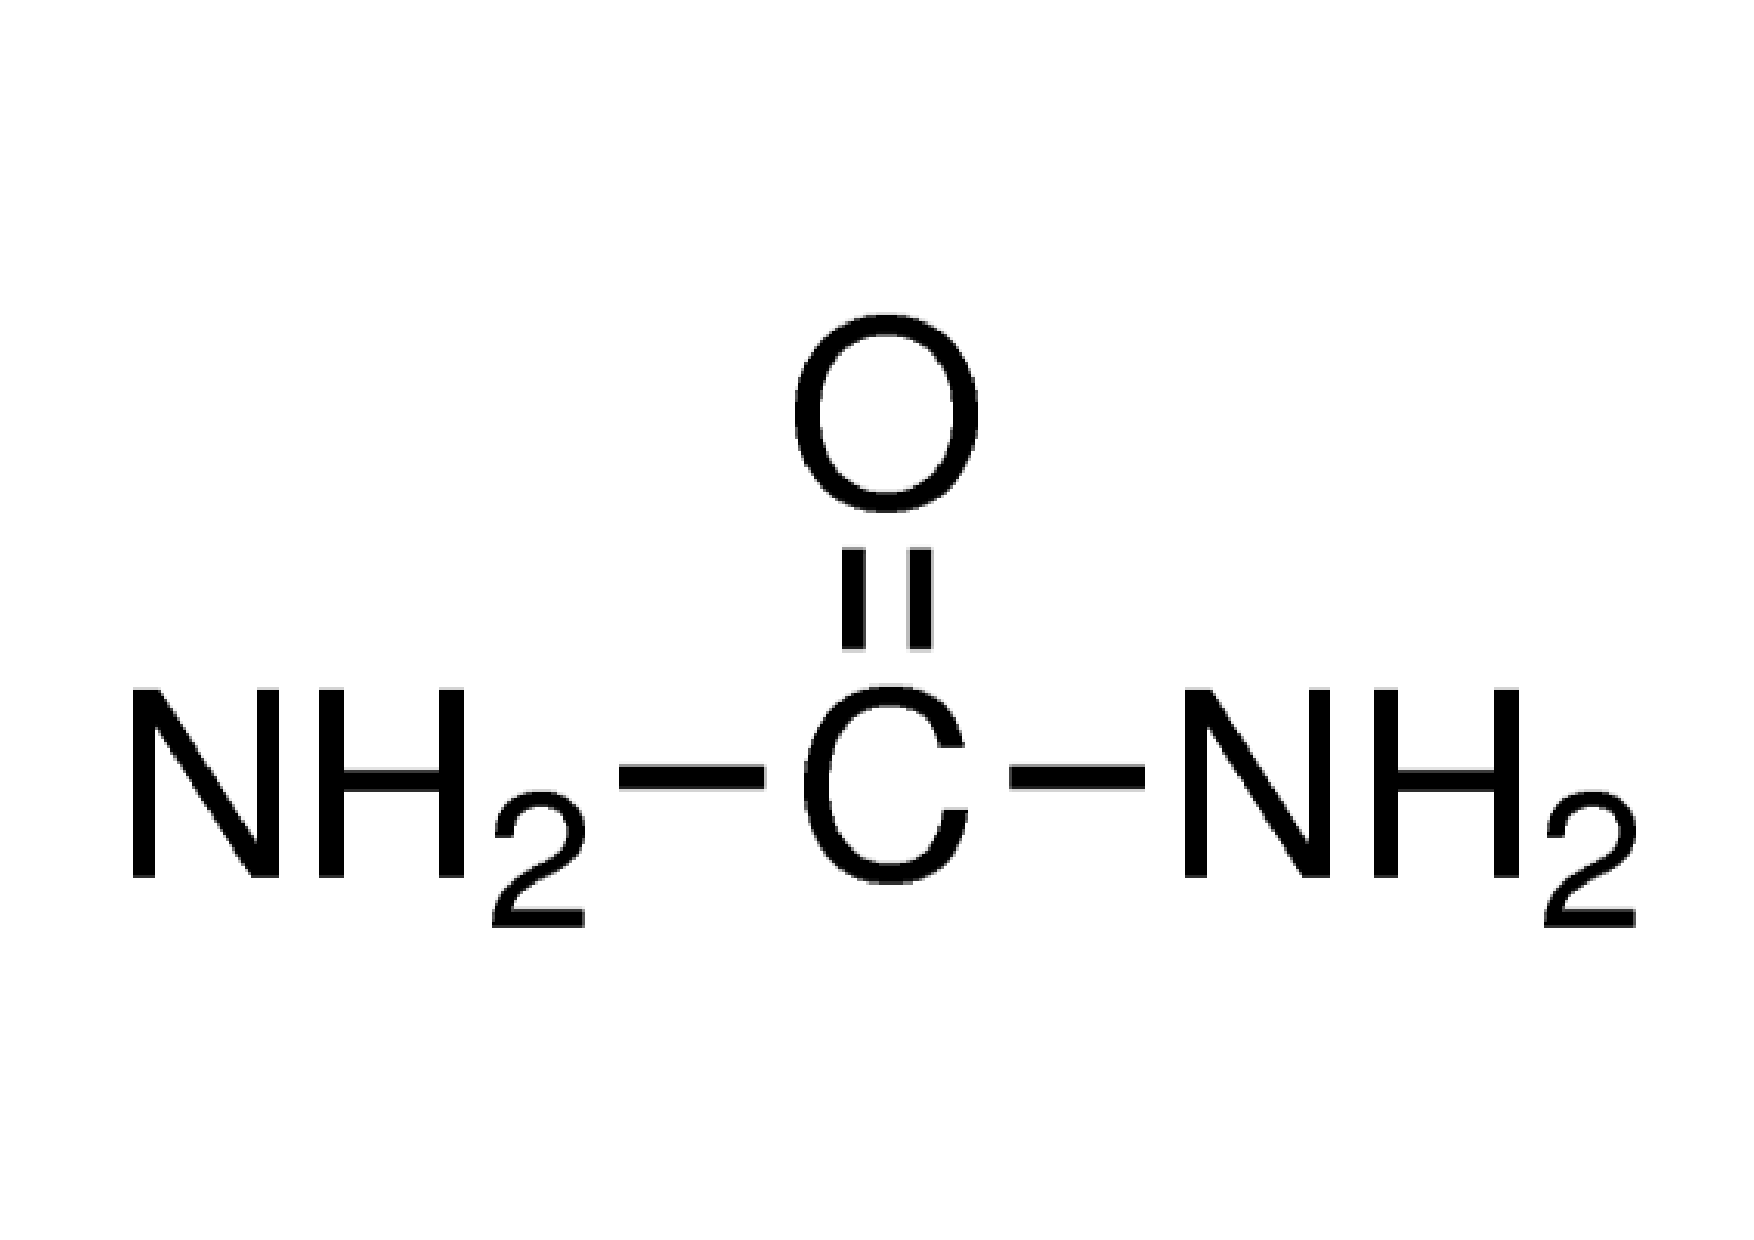
\includegraphics[width=4cm]{./images/urea}
% \caption{Structure of urea(CAS number is 57-16-6). Image taken from \cite{_urea_2014}}
% \end{figure}
% 
% \begin{figure}
% \centering
%   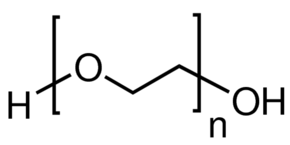
\includegraphics[width=4cm]{./images/poly(ethylene-glycol)}
% \caption{Structure of PEG (CAS number 25322-68-3). Image taken from \cite{_polyethylene_2014}}
% \end{figure}
%%%%%%%%%%%%%%%%%%%%%%%% molecules in structure formulas %%%%%%%%%%%%%%%%%%%%%%%% 
\paragraph{The etching solution} 

Many etching processes of Cu foils base of phosphoric acid. It is ``a clear colorless liquid or transparent crystalline solid. The pure solid melts at \SI{42.35}{\celsius} and has a density of \SI{1.834}{\g\per \cubic\cm}. Liquid is usually an 85\% aqueous solution. Shipped as both a solid and liquid. Corrosive to metals and tissue. Used in making fertilizers and detergents and in food processing.''\cite{_7664-38-2_2014} Sometimes refered to as ortho-phosphoric-acid. There are different additives such as PEG, Isopropanol or Butanol/Ethanol. These are used to gain a better control of the etching process. 

One may add PEG for reduced oxygen bubbling during the process (compare fig. \ref{oxygen-pitting})\cite{stables_report_2008,chang_superpolishing_2003}. Isopropanol and Ethanol are introduced for a more stable current density. HEDP increases the critical current density in phosphoric acid solutions\cite{jinshan_electrochemical_2004} and therefore the reaction rate.

Here (table \ref{tab:etching-recipes}), some of the etching recipes are given as reported in literature. They all have been used to electrochemically polish the Cu foil prior to graphene or boron nitride growth.
%%%%%%%%%%%%%%%%%%%%%%%%%%%%%%%%%%%%%%%%%%%%%%%%%%%%%%%%%%%%%%%%%%%%%%%%%%%%%%%%%%%%%%%%%%%%%%%%%%%
% \begin{table} \centering
% \caption{Table with some of the found etching recipes}
%  \begin{tabular}{cccccccc}
% 					&$H3PO_4$[\SI{}{\milli\liter}]&$H_2O$[\SI{}{\milli\liter}]&2-Propanol[\SI{}{\milli\liter}]&Ethanol[\SI{}{\milli\liter}]&Butanol[\SI{}{\milli\liter}]&Urea[\SI{}{\gram}]& (P)EG[\SI{}{\milli\liter}]\\
%   \cite{bin_zhang_low-temperature_2012} & 50     & 100  & 10        & 50    & ---   & 1   &  ---\\
%   \cite{stables_report_2008}		& 85	 & ---  & ---	    & ---   & 15    & --- &  ---\\
%   \cite{luo_effect_2011}		& 300	 & ---  & ---	    & ---   & ---   & --- &  100\\
%  \end{tabular}
% \label{tab:etching-recipes}
% \end{table}

\begin{table}[h] \centering
\caption{Table with some of the found etching recipes.}
 \begin{tabular}{lcccc}
	& unit & \cite{bin_zhang_low-temperature_2012} & \cite{stables_report_2008} & \cite{luo_effect_2011} \\ \hline \hline
$H3PO_4$	&[\SI{}{\milli\liter}]	& 50	& 85	& 300 \\
$H_2O$		&[\SI{}{\milli\liter}]	& 100	& ---	& --- \\
2-Propanol	&[\SI{}{\milli\liter}]	& 10	& ---	& --- \\
Ethanol		&[\SI{}{\milli\liter}]	& 50	& ---	& --- \\
Butanol		&[\SI{}{\milli\liter}]	& ---	& 15	& --- \\
Urea		&[\SI{}{\gram}]		& 1	& ---	& --- \\
(P)EG		&[\SI{}{\milli\liter}] 	& ---	& ---	& 100 \\
  \end{tabular}
\label{tab:etching-recipes}
\end{table}

%%%%%%%%%%%%%%%%%%%%%%%%%%%%%%%%%%%%%%%%%%%%%%%%%%%%%%%%%%%%%%%%%%%%%%%%%%%%%%%%%%%%%%%%%%%%%%%%%%%
\paragraph{Notes to etching recipes}
 \begin{itemize}
  \item[\cite{bin_zhang_low-temperature_2012}] A large copper plate is used as cathode. Alligator clamps are used to apply a voltage of \SIrange{3}{6}{\volt} between the foil and the plate. The foil is used as anode (+). After \SI{1}{\minute} the foil is taken out and rinsed with deionized water, further washed with ehtanol, and then blow dried with nitrogen.
  \item[\cite{stables_report_2008}] Mechanically polished with silicon carbide paper (wet-dry / \SIrange{1200}{6000}{})
  \item[\cite{luo_effect_2011}]
    \begin{itemize}
       \item rough polished with fine metal paste, cleaning in ethanol with sonication 
       \item soldlered to metal wire, covered with silicone gel on back, edges and corners
       \item etching in solution, foil used as work- (+) and copper plate as counter-electrode (-) 
       \item \SIrange{1}{2}{\volt} for \SI{0.5}{\hour} 
       \item wash with deionized water with sonication, neutralize acid remnants with amonia solution (\SI{1}{\percent})
       \item wash with ethanol and blow dry with nitrogen, remove silicone gel and store in ethanol
    \end{itemize}
 \end{itemize}

 %  \item 
% \begin{table}[h!]
% \centering
%   \begin{tabular}{lll} 
%   HEDP & \SI{30}{\percent} & \SI{60}{\ml} \\
%   $H_3PO_4$ & \SI{30}{\percent} & \SI{60}{\ml}\\
%   $H_2O$ & \SI{40}{\percent} & \SI{80}{\ml}\\
%   PEG & \SI{1000}{ppm} & \SI{0,2}{\ml}\\
%  \end{tabular}
% \caption{Etching recipe knowkn source}
% \end{table}

%  Removal rates are about \SI{1.8}{\mu \meter \per \min}

\begin{figure}[h]
 \begin{center}
  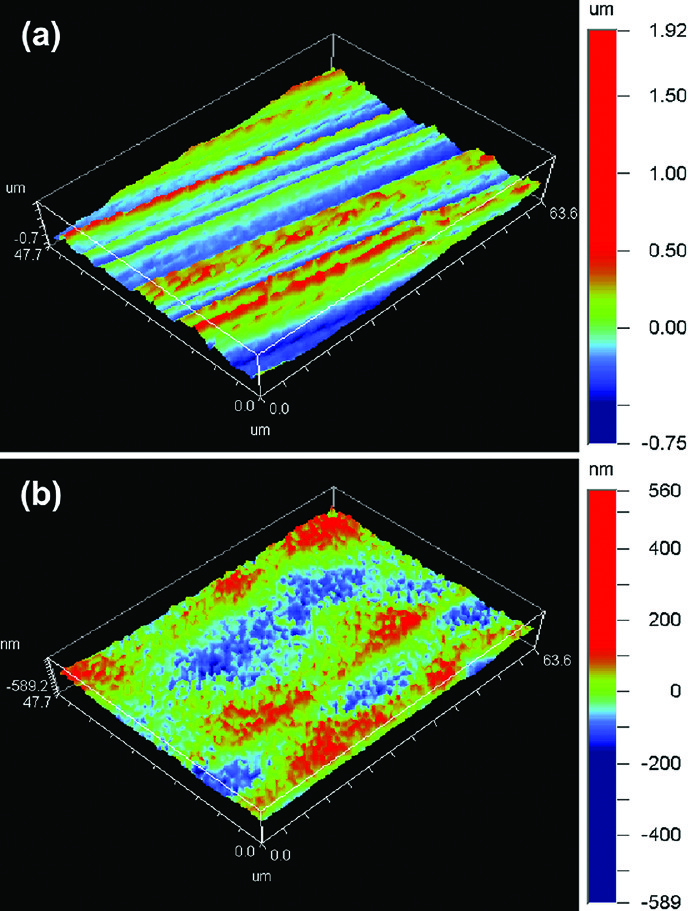
\includegraphics[height=6cm]{./images/0fcfd512d196815269000000-fig1.jpg}
 \end{center}
\caption{Height profiles before (a) and after (b) etching with solution \cite{bin_zhang_low-temperature_2012}.}
\end{figure}
\begin{figure}[h]
 \begin{center}
  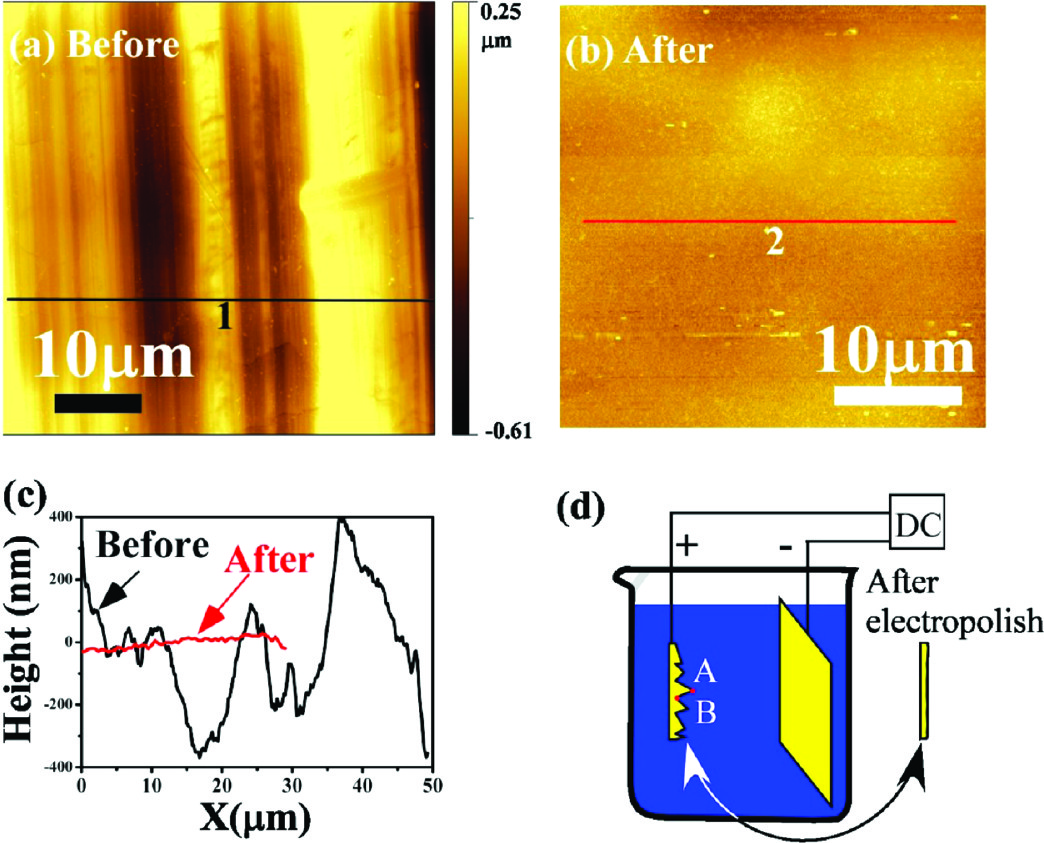
\includegraphics[height=6cm]{./images/cm1028854-fig2.jpg}
 \end{center}
\caption{(a-b) Copper foil before and after etching with recipe \cite{luo_effect_2011} with corresponding height profiles (c). The experimental setup for polisching the foils is shown in (d)}
\label{figure:luo-effect_2011}
\end{figure}

\paragraph{Used solutions}\index{electrochemical polishing!Used solutions}
Within this work, Cu-foil polishing will be done with recipe I broken down in table \ref{table:used-etching-solutions}
\begin{table}\centering
\caption{Used etching solutions (compare \cite[130]{jinshan_electrochemical_2004}). Note the change in the removal rate due to higher limiting currents in the solution.}
 \begin{tabular}{lcc}
  & I & II \\ \hline \hline
  $\SI{85}{\percent} H_3PO_4$ & 70 & 100 \\
  Ethylene-gylcol & 5 & 0 \\
  Deionized water & 25 & 0 \\ \hline
  Potential [\SI{}{\V}] & \multicolumn{2}{c}{\SI{1.2}{}} \\
  Current [\SI{}{\mA}] & 46 & 12\\
  Roughness [\SI{}{\nm}] & \multicolumn{2}{c}{\SI{5}{}} \\
  Removal rate [\SI{}{\micro\meter\per\minute}] & \SI{1,0}{} & \SI{0,26}{}\\
 \end{tabular}
\label{table:used-etching-solutions}
\end{table}
The given roughness in table \ref{table:used-etching-solutions}is much lower compared to references (\SI{61}{\nm})\cite[2]{bin_zhang_low-temperature_2012} that did the polishing with another recipe (compare table \ref{tab:etching-recipes}). Although the roughness is higher, optical profiler images indicate removed striations and a smoother surface compared to the as-bought foils (\SI{218,56}{\nm})\cite[2]{bin_zhang_low-temperature_2012}.

\paragraph{The etching process}
The first attempt to etch the Cu-foil was performed with the $5\%_{vol}$ EG, $25\%_{vol}\,H_2O$ filled up with phosphoric acid. The etching was performed in a \SI{200}{\ml} beaker, filled with \SI{150}{\ml} etching solution. The setup is as depicted in fig \ref{figure:luo-effect_2011}. The potential was adjusted to be \SI{1.2}{\V}. The current through the solution changes and is typically highest when the etching process started. After some minutes, the foil starts to change. The reflectivity changes, making the foil - shiny before etching - a little dull. After some additional time the foil begins to reflect light better again. This is the moment where the etching process is interrupted. The time inside the etching solution depends on the handling - but was usually $\geq \SI{2}{\hour}$. 

One has to be careful if reproducable results are needed. During the etching process (as more and more copper settles on the counter electrode), the current and therefore the etching rate decrease continuously. When the beaker is moved, some of the debris on the electrode changes (the electrode's) surrounding and the etching rate changes. Front- and backside of the foil are suspect to different etching rates - at least the foil has different appearance on its sides. The back side is generally more flat, because the side facing the counter-electrode always shows some additional protrusions.

\paragraph{After etching treatment}
The foil is taken out and cleaned from remaining etchants with purified water first and isopropanol afterwards. Foils can be stored in Ethanol to avoid oxidation. 

To further improve the quality of the foil, one can follow the documented recipe for annealing the foil in a $H_2$ atmosphere (\SI{10}{sscm}, \SI{1000}{\celsius}, 30min)\cite{kim_synthesis_2012} to increase the copper grain size and further smoothen the surface. 

So prepared foils are investigated in XPS (compare figure \ref{fig:xps-self-grown}) - (discussion of peaks can be found inside the textx and in \cite[8]{stables_report_2008}).

\paragraph{SEM}
After the etching process one foil is investigated in SEM. It was stored for one day in isopropanol and blown dry with nitrogen. 

\begin{figure}[h]
  \begin{center}
   \includegraphics[height=6cm]{../Daten/SEM/160317-Domenik/Domenik_16031715.jpg}
   \includegraphics[height=6cm]{../Daten/SEM/160317-Domenik/Domenik_16031717.jpg}
  \end{center}
 \caption{SEM image of etched copper foil. Different contrast suggests different grain-orientation within the surface. a) Larger (\SI{570}{\micro \meter}x\SI{380}{\micro \meter}) image schowing the contrast of different grains in the copper-foil, b) zoom (\SI{18}{\micro \meter}x\SI{12}{\micro \meter})} to a area with two different contrasts and their border.
 \label{SEM-gb}
\end{figure}

One can see (figure \ref{SEM-gb}) that the surface imaged in different intensities which correspond to the different orientation of the copper grains within the foil\cite{wu_effects_2015}. The grainsize may range from just a few \SI{}{\micro \meter} to several hundret \SI{}{\micro \meter} and in some cases even \SI{}{\milli \meter}. The grains are separated by grain boundaries. Large grains are preferred for growing graphene on copper foils because grain boundaries are subject to inhomogenities within the graphene layer and provide a route for unwanted surface chemistry (copper oxidation for example). These effect can be also be used to highlight grain boundaries as shown in \cite{wu_effects_2015}.

Although not very rough, the copper foil shows surface variation. While some areas of the sample show some wavy surface, whereas other are much flatter and appear in a different intensity (figure \ref{SEM-surface}).

Neither estimation on the grainsize nor guesses for their absolute orientation have been done due to the lack of EBSD-data in the SEM setup.

\begin{figure}[h]
  \begin{center}
   \includegraphics[height=6cm]{../Daten/SEM/160317-Domenik/Domenik_16031700.jpg}
   %\includegraphics[height=6cm]{../Daten/SEM/160317-Domenik/Domenik_16031717.jpg}
  \end{center}
 \caption{SEM image that shows different surface morphologies (\SI{5.6}{\micro \meter}x\SI{3.7}{\micro \meter})}
 \label{SEM-surface}
\end{figure}

\paragraph{AFM}
\begin{figure}[h]
 \centering
 \includegraphics[width=0.4\textwidth]{../Daten/AFM/2015-01-15/as_bought0000.jpg}
 \includegraphics[width=0.4\textwidth]{../Daten/AFM/2015-01-15/as_bought0001.jpg}
 \caption{AFM image of the \SI{0.25}{\mm} copper foil as bought from alfa aesar, RMS$\approx$\SI{13}{\nm}, contrast \SI{100}{\nm} ($\approx$ RMS \SI{9}{\nm}, contrast \SI{70}{\nm} in the right image)}
 \label{fig:foil-afm-as-bought}
\end{figure}

Figure \ref{fig:foil-afm-as-bought} shows the striations that stem from the production process (from top to buttom).
\begin{figure}[h]
 \centering
 \includegraphics[width=0.4\textwidth]{../Daten/AFM/2015-01-15/polished0000.jpg}
 \includegraphics[width=0.4\textwidth]{../Daten/AFM/2015-01-15/polished0001.jpg}
 \caption{AFM image of a copper foil polished 5h (according to table \ref{tab:used-etching-solution}), RMS$\approx$\SI{9}{\nm} in the left image, contrast \SI{100}{\nm} ($\approx$\SI{3}{\nm} in the right image, contrast \SI{70}{\nm})}
 \label{fig:foil-afm-polished}
\end{figure}
After etching ($U=1.2V$,I=\SIrange{120}{250}{\mA}) for \SI{5}{\hour} in a solution (shown in table \ref{tab:used-etching-solution}) the striations have gone and the RMS value decreased by \SIrange{30}{45}{\percent} and an increase in foil quality is obvious even with bare eyes. Figure \ref{fig:foil-afm-as-bought} and \ref{fig:foil-afm-polished} show AFM images in the same size and contrast - before and after etching.
The circular hole is an effect of bubbles in the etching process where the bubble affects the rate of etching. The over all structure changes from a heterogenous sample height to a flat height contribution with only a little amount of defects. Those are sufficiently seperated in space to exhibit flat regions where the h-BN may grow unperturbated.

\begin{table}
\centering
\caption{Volume and mass fractions for copper foil etching solution.}
\begin{tabular}{lcccc}
		&unit	&$H_3PO_4$ (85\%)&	EG	&	$H_2O$	\\
Dichte $\rho$   &[$g/cm^3$]	&	1.87	&	1.11	&	1.00	\\
$1/rho$		&[$cm^3/g$]	&	0.54	&	0.90	&	1.00	\\
Anteil 		& \%		&	70	&	5	&	25	\\ \hline
Menge gesamt    &[$cm^3$]	&		\multicolumn{3}{c}{150} 	\\
Menge anteilig  &[$cm^3$]	&	105.00	&	7.50	&	37.50	\\
Gewicht         &[g]		&	196.35	&	8.33	&	37.50	\\
\end{tabular}
\label{tab:used-etching-solution}
\end{table}

\paragraph{not done yet - maybe future?}
Some foil has been mechanically polished with 4k paper and several hours of Syton polishing. The roughness of these samples has been investigated also in AFM. These are compareable to the chemically polished ones, but are always slightly higher by $\approx 10\%$. Sometimes unwanted new scratches appear after mechanical polish.

\paragraph{STM}
The bought and chemically polished foils are mounted on a sample holder and loaded into the load lock. It is evacuated for \SIrange{2}{3}{\hour}, afterwards the valve is opened to the chamber. During transfer, no noteable increase in the base pressure is noted. The sample is put on the parking slot.

The sample was initially degased with slowly increasing temperatures to remove adsorbats like $CO, CO_2$ and $H_2O$.

After some time of degassing, the sample was prepared with repeated sputter and anneal cycles. The annealing temperatures were increased up to \SI{800}{\degreeCelsius}. 
After that procedure, the sample was cooled down and observed in STM.

\begin{figure}[h!]
 \centering
 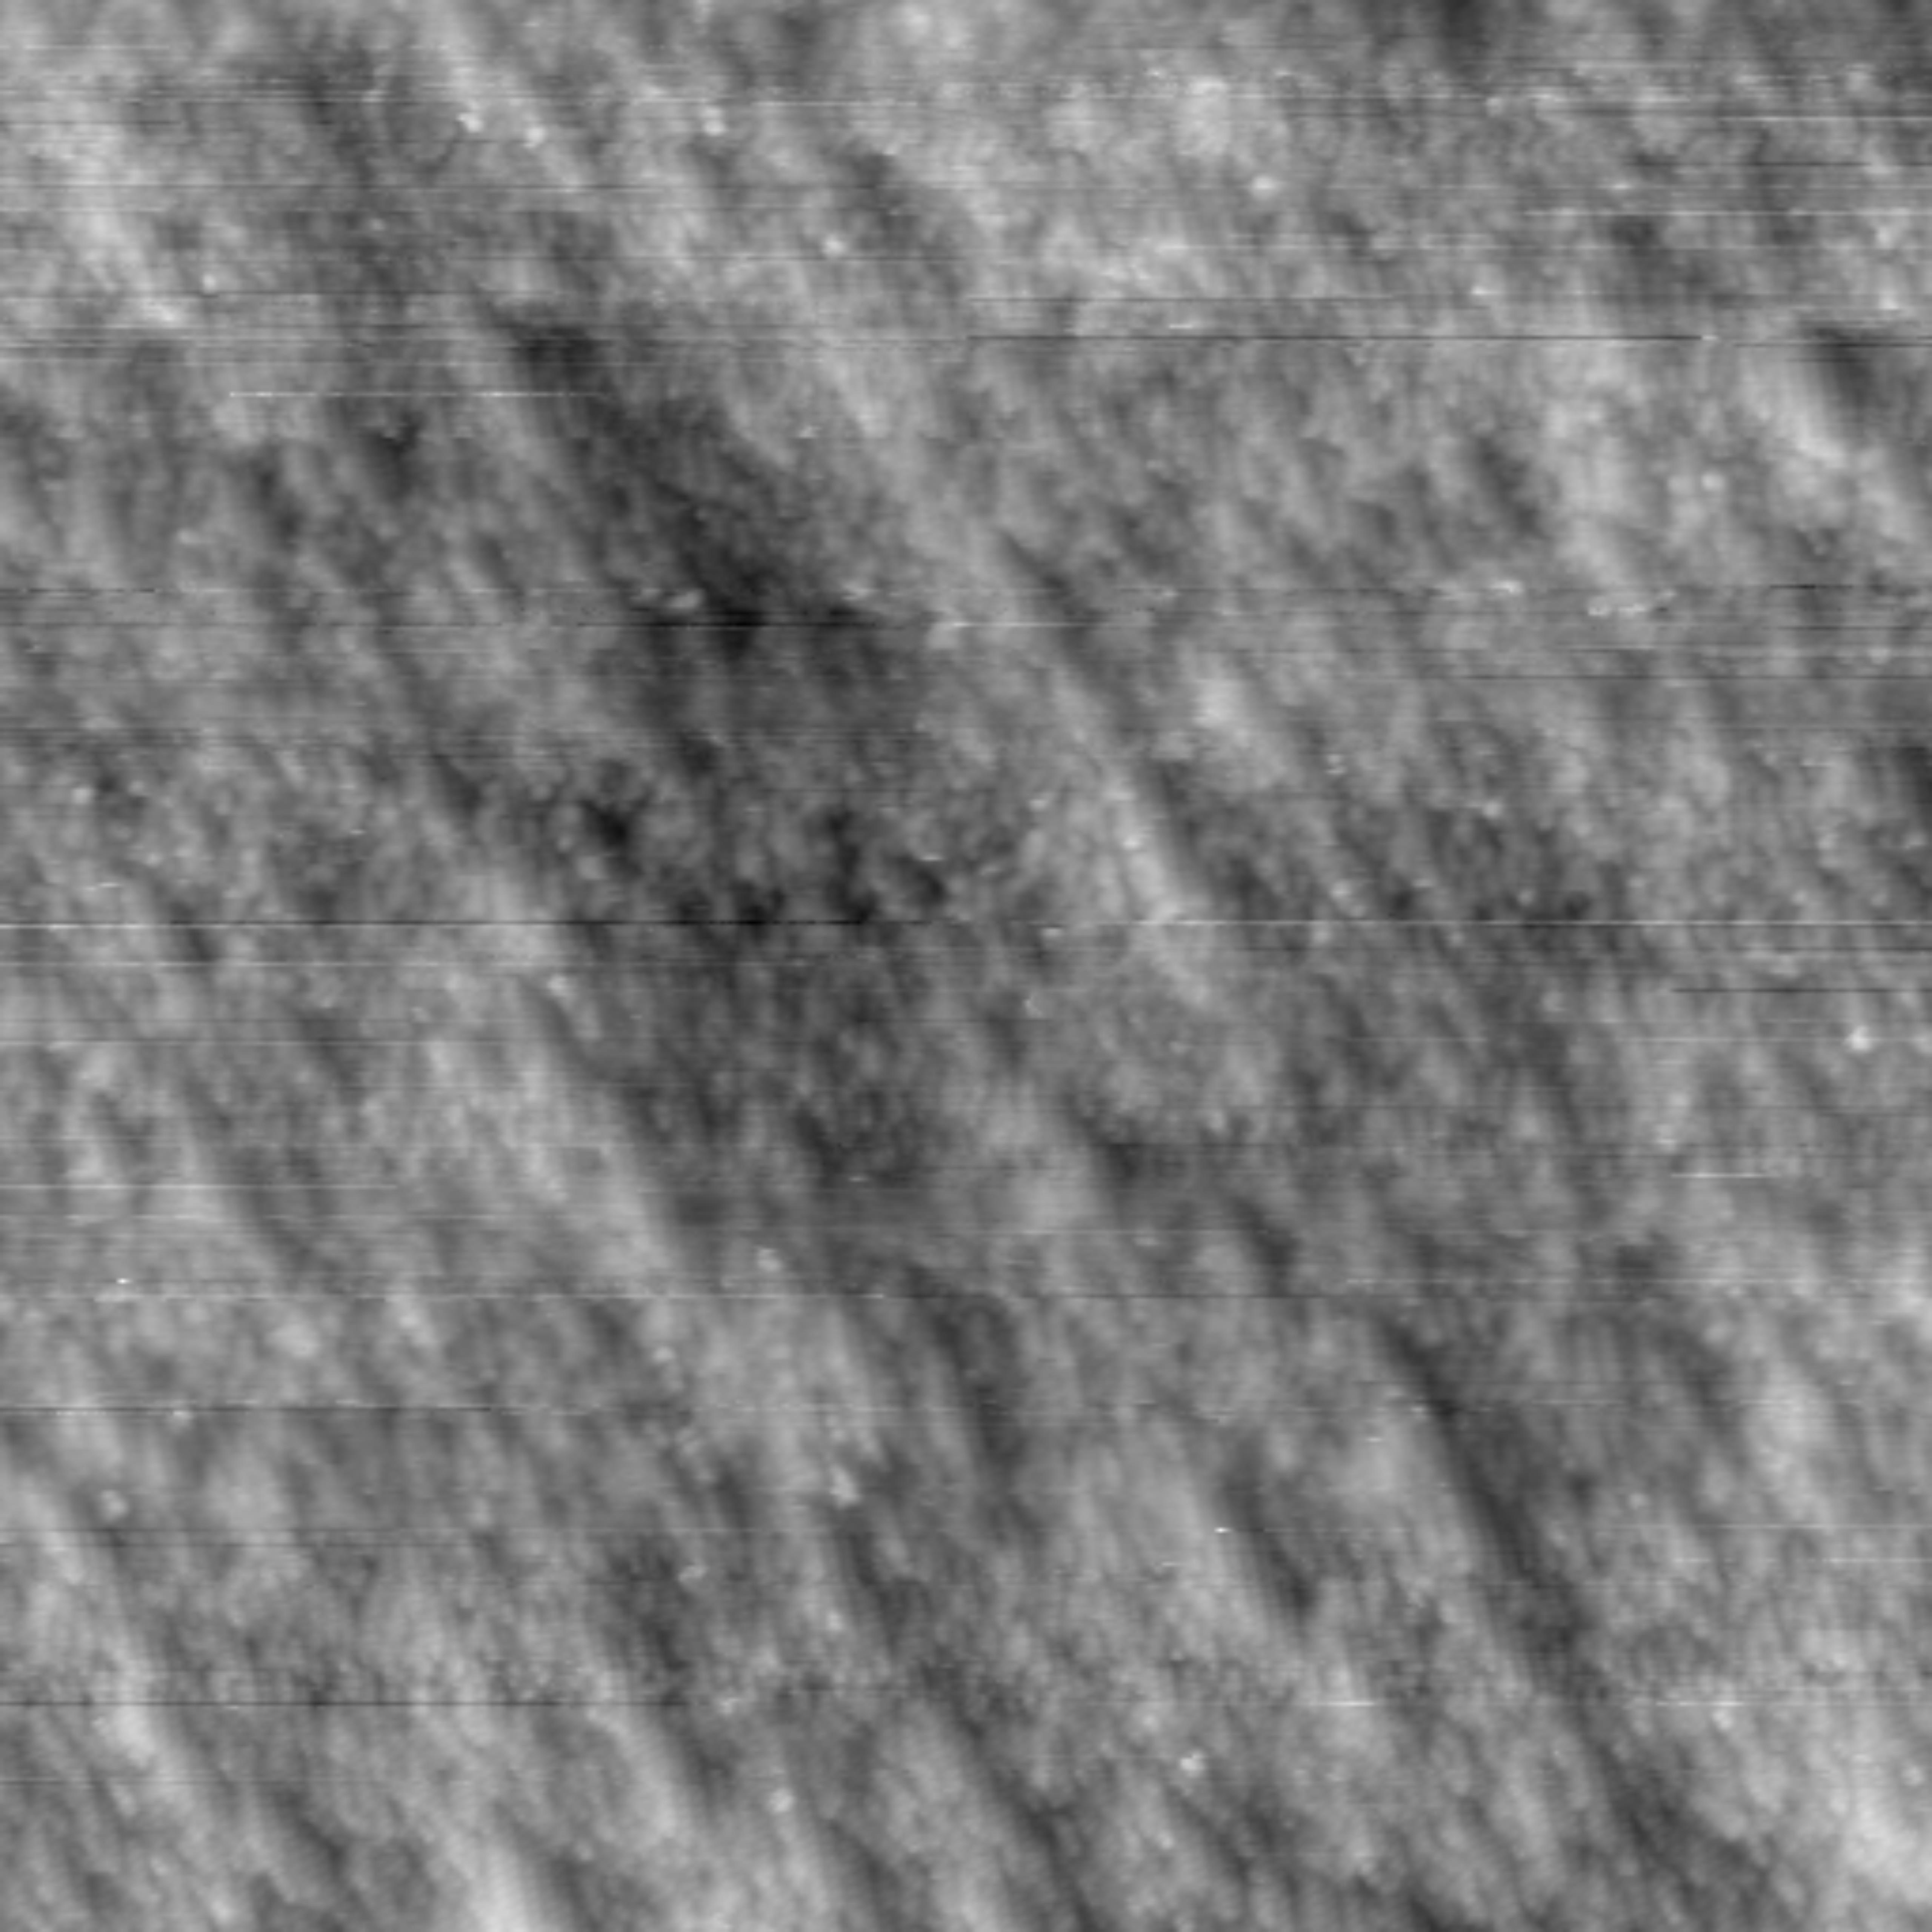
\includegraphics[width=0.5\textwidth]{./images/F150331-125720.jpg}
 \caption{Cu-foil after repeated sputtering and annealing cycles. A rather flat area is shown with no larger corrugation. The roughness is \SI{72}{\pico\meter}.}
 \label{fig:cu-foil-clean}
\end{figure}

A first look onto the sample shows a quite heterogen surface. While quite flat areas with a typical roughness of $\approx \SI{70}{\pico\meter}$ exist, areas with very large corrugations $\geq \SI{100}{nm}$ are hard to scan and bad places for h-BN growth etc.
%   \subsection{STM of 0.25mm Cu-foils}
%      The bought and chemically polished foils are mounted on a sample holder and loaded into the load lock. It is evacuated for \SIrange{2}{3}{\hour} and the valve is opened to the chamber. During transfer, no noteable increase in the base pressure is noted. The sample is put on the parking slot.

The sample was initially degased with slowly increasing temperatures to remove adsorbats like $CO, CO_2$ and $H_2O$.

After some time of degassing, the sample was prepared with repeated sputter and anneal cycles. The annealing temperatures were increased up to \SI{800}{\degreeCelsius}. 
After that procedure, the sample was cooled down and observed in STM.

\begin{figure}[h!]
 \centering
 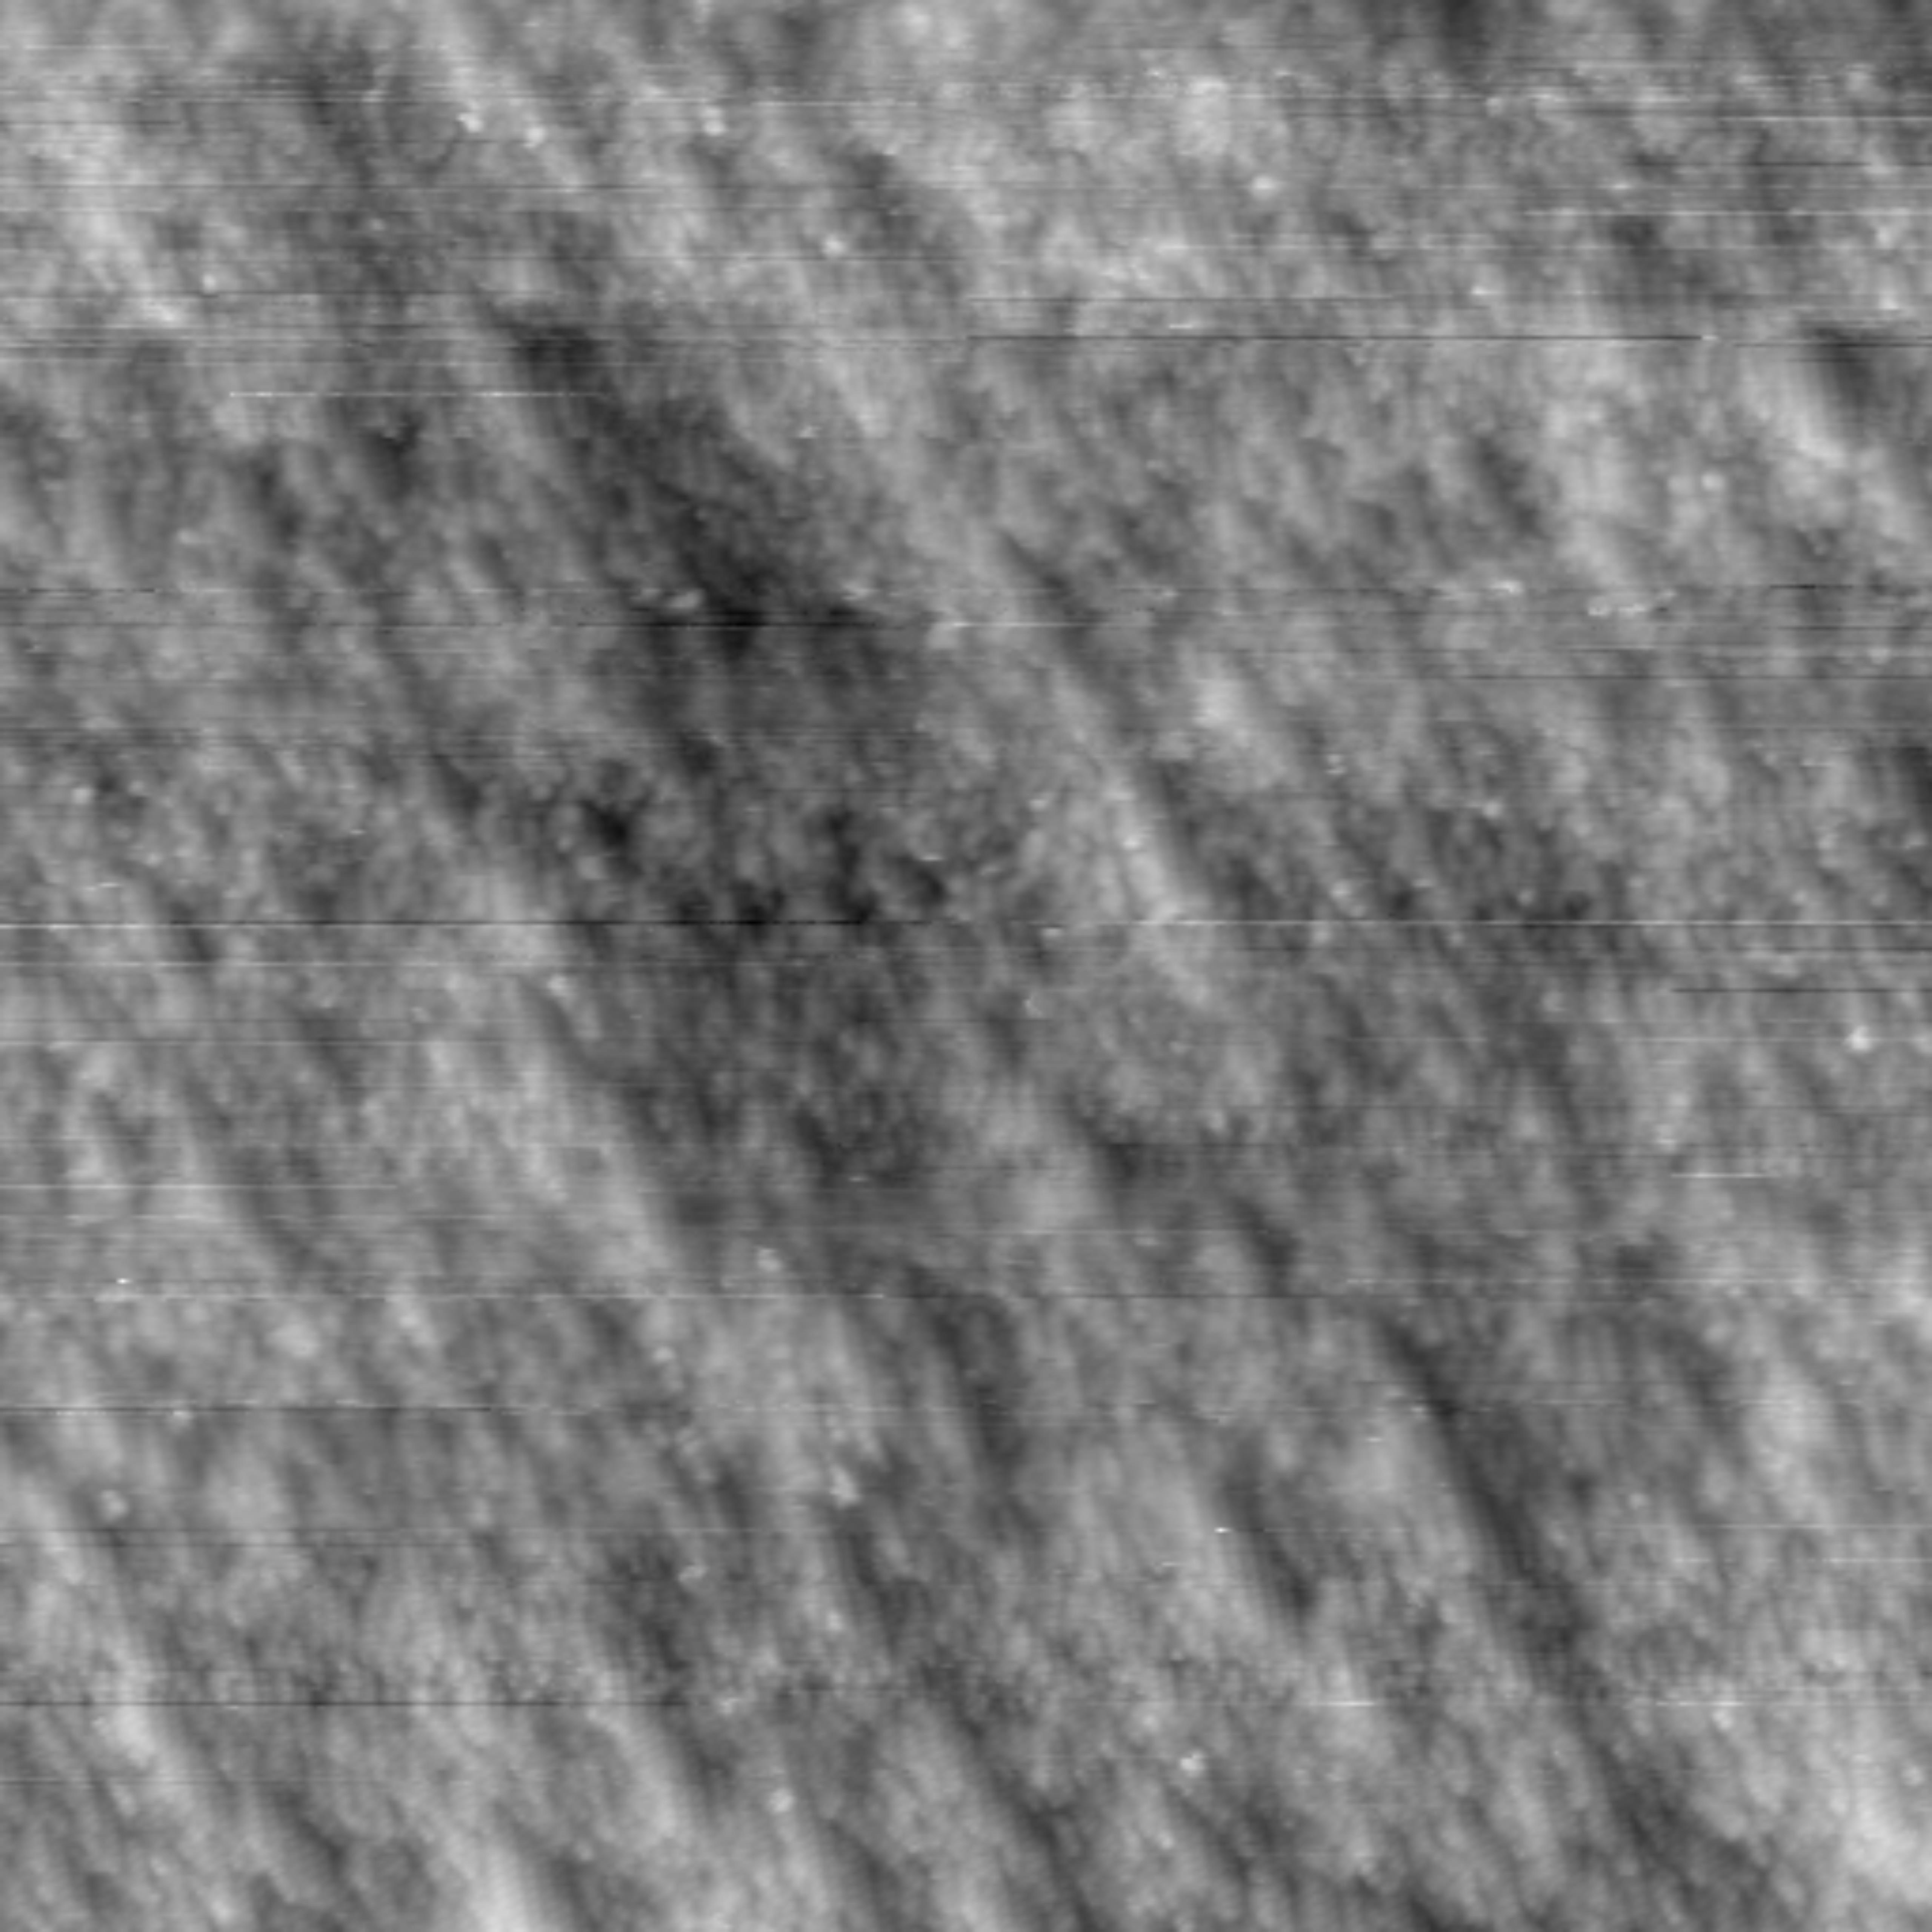
\includegraphics[width=0.5\textwidth]{./images/F150331-125720.jpg}
 \caption{Cu-foil after repeated sputtering and annealing cycles. The roughness is about \SI{72}{\pico\meter}}
 \label{fig:cu-foil-clean}
\end{figure}

A first look onto the sample shows a quite heterogen surface. While quite flat areas with a typical roughness of $\approx \SI{70}{\pico\meter}$ exist, there are also areas with very large corrugations $\geq \SI{100}{nm}$.
%   \subsection{AFM of 0.25mm Cu-foils}
%      \paragraph{AFM}
\begin{figure}[h]
 \centering
 \includegraphics[width=0.4\textwidth]{../Daten/AFM/2015-01-15/as_bought0000.jpg}
 \includegraphics[width=0.4\textwidth]{../Daten/AFM/2015-01-15/as_bought0001.jpg}
 \caption{\SI{0.25}{\mm} as bought from alfa aesar, RMS$\approx$\SI{13}{\nm}, contrast \SI{100}{\nm} ($\approx$ RMS \SI{5}{\nm}, contrast \SI{70}{\nm} in the smaller image)}
\end{figure}
One can see the striations that stem from the production process (from top to buttom).
\begin{figure}[h]
 \centering
 \includegraphics[width=0.4\textwidth]{../Daten/AFM/2015-01-15/polished0000.jpg}
 \includegraphics[width=0.4\textwidth]{../Daten/AFM/2015-01-15/polished0001.jpg}
 \caption{\SI{0.25}{\mm} polished 5h in in 75/20/5 phosphoric acid, RMS$\approx$\SI{9}{\nm} in the over all image, contrast \SI{100}{\nm} ($\approx$\SI{5}{\nm} in the smaller image, contrast \SI{70}{\nm})}
\end{figure}
After etching ($U=1.2V$,I=\SIrange{120}{250}{\mA}) \SI{5}{\hour} in a solution \SI{75}{\percent} \SI{20}{\percent} \SI{5}{\percent} (Phosphoric acid, purified water, EG) the striations have gone and the RMS value decreased by \SIrange{30}{45}{\percent} (protrusions due to dirt in the image are counted).
The circular hole is an effect of bubbles in the etching process where the bubble affects the rate of etching. The over all structure changes from a very fuzzy and heterogenous sample height to a flat height contribution with only a little amount of defects. Those are sufficiently seperated in space to exhibit flat regions where the h-BN may grow unperturbated.
\begin{table}
\centering
\caption{Volume and mass fractions for copper foil etching solution.}
\begin{tabular}{lccc}
			&$H_3PO_4$ (85\%)&	EG	&	$H_2O$	\\
Dichte [$g/cm^3$]	&	1.87	&	1.11	&	1.00	\\
$1/rho$			&	0.54	&	0.90	&	1.00	\\
Anteil \%		&	70	&	5	&	25\\
Menge gesamt [$cm^3$]	&		\multicolumn{3}{c}{150} \\
Menge anteilig [$cm^3$]	&	105.00	&	7.50	&	37.50	\\
Gewicht [g]		&	196.35	&	8.33	&	37.50	\\
\end{tabular}
\end{table}

Some foil has been mechanically polished with 4k paper and several hours of Syton polishing. The roughness of these samples has been investigated also in AFM. These are compareable to the chemically polished ones, but are always slightly higher by $\approx 10\%$. Sometimes unwanted new scratches appear after mechanical polish.
  \section{STM of BN on Cu-foil(0.25mm)}
     % Beamtime April 2015
Further experiments were carried out to increase the cleanlyness of the h-BN on the polycrystalline copper foil. To reduce the amount of elements coming from the body of the foil it is repeatedly sputtered and annealed to temperatures as high as \SI{800}{\degreeCelsius}. This may have also an improving influence on the grainsize and amount of corrugation. Several attempts have been made which are described in summary below.
%%%%%%%%%%%%%%%%%%%%%%%%%%%%%%%%%%%%%%%%%%%%%%%%%%%%%%%%%%%%%%%%%%%%%%%%%%%%%%%%%%%%%%%%%%
\begin{itemize}
 \item After cleaning, the sample is inverstigated in STM. The foil shows a inhommogenous topography, with parts of the sample showing very flat regions (figure \ref{fig:30-31.03}) while others still remain heavily corrugated.
\end{itemize}
% -----------BILDER ---- DISKUSSION: 30.03/31.03
\begin{figure}[h!]
 \centering
 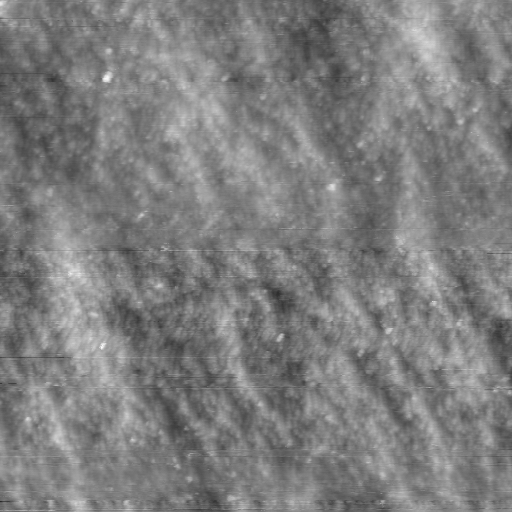
\includegraphics[width=0.5\textwidth]{./images/F150331-124839.png}
 \caption{Cu-foil after repeated sputtering and annealing cycles. Roughness $\approx \SI{100}{\pico\meter}$. Compare figure \ref{fig:cu-foil-clean}.}
 \label{fig:30-31.03}
\end{figure}
%%%%%%%%%%%%%%%%%%%%%%%%%%%%%%%%%%%%%%%%%%%%%%%%%%%%%%%%%%%%%%%%%%%%%%%%%%%%%%%%%%%%%%%%%%
\begin{itemize}
 \item Before dosage the sample was kept at \SI{800}{\degreeCelsius} for another 10 minutes.
Borazine was dosed for 5 minutes with a pressure of \SI{1e-7}{\milli \bar} with the sample kept at temperatures of \SI{850}{\degreeCelsius}. Afterwards the sample was kept at this temperature for another minute.
\end{itemize}
%  -----------BILDER ---- DISKUSSION: 15.04
% \begin{figure}
%  \centering
%  \includegraphics[width=0.5\textwidth]{./images/}
%  \caption{}
%  \label{fig:15.04}
% \end{figure}
%%%%%%%%%%%%%%%%%%%%%%%%%%%%%%%%%%%%%%%%%%%%%%%%%%%%%%%%%%%%%%%%%%%%%%%%%%%%%%%%%%%%%%%%%%
\begin{itemize}
 \item The sample was sputtered and annealed several times to temperatures of \SI{800}{\degreeCelsius}. Before the dosage it was held 5 minutes at \SI{750}{\degreeCelsius}. Borazine was dosed with the same pressure as before (\SI{1e-7}{\milli \bar}) but for 1min and at a lower temperature of \SI{750}{\degreeCelsius}. After the preparation the sample was kept at \SI{750}{\degreeCelsius} for another 1 minute. It was cooled down slowly (shown in figure \ref{fig:16.04}.
\end{itemize}

\begin{figure}
 \centering
 \includegraphics[width=0.5\textwidth]{./images/F150416-192611.png}
 \caption{STM image after 4\,L of borazine dosage on a \SI{800}{\degreeCelsius} hot Cu-foil surface. A little h-BN island can be seen on a largely uncovered copper foil background (lower right). 44x44nm image size}
 \label{fig:16.04}
\end{figure}
% -----------BILDER ---- DISKUSSION: 16.04
% %%%%%%%%%%%%%%%%%%%%%%%%%%%%%%%%%%%%%%%%% false preparation %%%%%%%%%%%%%%%%%%%%%%%%%%%%%%
% The next preparation step was started with an intense cleaning step of the copper foil. It was sputtered and annealed to \SI{750}{\degreeCelsius} twice and then kept at \SI{830}{\degreeCelsius} for 2 hours. After this it was sputtered and annealed to \SI{750}{\degreeCelsius} for 1 minute before the borazine was dosed. Unfortunatly the exact amount of borazine could not be determined, the pressure increased to \SI{1e-4}{\milli \bar} for a very short time, so that the dosage was interrupted well below 1 minute. It was again hold at the temperature for another minute and was cooled down very slow (\SIrange{1}{3}{\kelvin \per \second}). The mass spectrum taken after deposition shows the highest peak not where the intact borazine molecule is located but somewhere to lower masses. This indicates that the borazine has decomposed.
% 
% -----------BILDER ---- DISKUSSION: 17.04
%%%%%%%%%%%%%%%%%%%%%%%%%%%%%%%%%%%%%%%%%%%%%%%%%%%%%%%%%%%%%%%%%%%%%%%%%%%%%%%%%%%%%%%%%%
\begin{itemize}
 \item The foil was sputtered and annealed 4 times with temperatures of \SI{800}{\degreeCelsius}. Borazine was dosed at \SI{2e-7}{\milli \bar} for \SI{2.5}{\minute}. The sample was kept at this temperature for another 5 minutes after dosing. The sample was cooled down slowly. Figure \ref{fig:15.04} shows some of the grown islands. The copper surface changes upon h-BN growth and the terrace width increases below the h-BN flakes. The typical facetting of the surface vanishes or can at least not be depicted because of the overgrowing h-BN (figure \ref{fig:23.04}). Due to nearby tip formings, the right side of the image is decorated with adsorbats, most likely from the tip itself - they appear as bright white spots in the image.
\end{itemize}
% -----------BILDER ---- DISKUSSION: 21.04
\begin{figure}
 \centering
 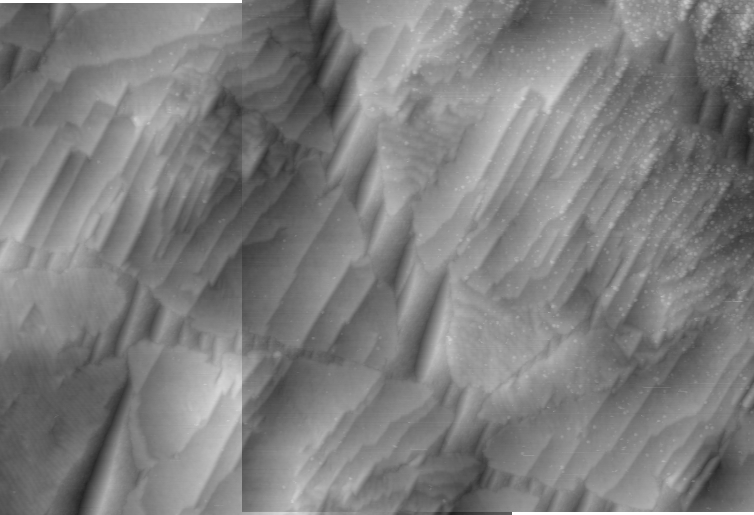
\includegraphics[width=\textwidth]{./images/150423-1008-1027}
 \caption{STM image of 22\,L boarazine dosed on a \SI{800}{\degreeCelsius} hot copper-foil surface. Serveral large islands can be seen that grow over Cu-foil step edges. Defiled right hand side of the image due to nearby tip forming. Overlay of two images. Image height: \SI{295}{\nm}}
\end{figure}

\begin{figure}
 \centering
 \includegraphics[width=0.5\textwidth]{./images/F150423-114214.jpg}
 \caption{STM image of island that overgrows Cu-foil facets.}
 \label{fig:23.04}
\end{figure}

%%%%%%%%%%%%%%%%%%%%%%%%%%%%%%%%%%%%%%%%%%%%%%%%%%%%%%%%%%%%%%%%%%%%%%%%%%%%%%%%%%%%%%%%%%
points to point out:
\begin{itemize}
 \item Look at Messzeit-April.ppt power point presentation
 \item Stufenh\"ohe
 \item Beschaffenheit der stufen/facetts $\rightarrow$ material transport mechanism/strength differs uner the h-BN compared to the bare cu-foil surface.
 \item Wechselwirkung BN-Wachstum und Facettenbildung
\end{itemize}

\paragraph{surface structure of h-BN on Cu-foil}
During experiments some ``new'' structure appeared (compare figure \ref{fig:h-BN-stripes-cu-foil}).


\begin{figure}
 \centering
 \subfigure[Molecules on copper foil surface - supposed be be covered with h-BN, maybe just free (maybe facetted) copper]{
 \includegraphics[width=0.5\textwidth]{./images/F150810-113456.jpg}
 }
 \caption{funny surface structure - oxygen overlayer ?- but not sure - maybe some very small (\SI{0.75}{\nm}) moire on a Cu(100) facet? Noise can be excluded due to the fact that the stripes do not occur on the molecules, but only on the substrate. Many deformed molecules visible $\rightarrow$ strong substrate interaction $\rightarrow$  no \textit{h}-BN ?}
 \label{fig:h-BN-stripes-cu-foil}
\end{figure}

  \section{XPS of self-grown h-BN/Cu-foils}
     %this file contains information on self-grown h-BN on the comercially bought copper foils
Copper foils with \SI{0.25}{\mm} were bought and repeatedly sputtered/annealed. Several grow cycles of h-BN via CVD of borazine were done.  The sample is transfered to the XPS-STM chamber and again sputtered/annealed serveral times to clean it properly.

The needed dosage of borazine to assemble a full monolayer of h-BN is derived via a combinated STM/XPS measurement. Several preparations were done to understand the growth behaviour of h-BN on the copper foil. Coverages are measured in STM while the chemical composition of the sample was assessed with XPS.
\begin{table}[h!]
\centering
\caption{Determination of the full monolayer borazine dosage. First a certainly saturated sample was prepared (I) and measured in XPS/STM. A sub-monolayer (II) was grown and compared to the monolayer STM and XPS results.}
 \begin{tabular}{cccccccc}
  & Prep. & Position    & Area [arb.u.] & FWHM  & Anode & Dosage  & Coverage\\ 
  &	  &	[eV]	& (XPS)		&[eV]	&Element&[L]	  & (STM) \\ \hline \hline
  \multirow{2}{*}{B1s} 	&I& 191.1 & 3776 & 1.35 & Mg & 4736 & \SI{100}{\percent}\\
    			&II& 191.1 & 1994 & 1.35 & Mg & 789 &\SI{53}{\percent}\\ \hline
  \multirow{2}{*}{N1s} 	&I& 398.7 & 5875 & 1.45 & Al  & 4736 & \SI{100}{\percent}\\
 			&II& 398.6 & 3183 & 1.43 & Al & 789 &\SI{54}{\percent}\\
 \end{tabular}
\end{table}

\begin{figure}[ht]
\centering
\subfigure[N1s]{
   \includegraphics[width=.45\textwidth]{./images/XPS-150314-N1s.jpg}
   }
\subfigure[B1s]{
   \includegraphics[width=.45\textwidth]{./images/XPS-150314-B1s.jpg}
   }
\subfigure[C1s]{
   \includegraphics[width=.45\textwidth]{./images/XPS-150314-C1s.jpg}
   }
\subfigure[Cu3s]{
   \includegraphics[width=.45\textwidth]{./images/XPS-150314-Cu3s.jpg}
   }
\caption{XPS spectra for ML h-BN/Cu-foil. The peaks are at their expected positions\cite{kidambi_situ_2014} and show no additional features. No remnants of sulfur or remaining oxygen could be found.}
\label{fig:xps-self-grown}
\end{figure}

When comparing the resulting coverage (STM coverage/XPS signal) (II) to the (saturated) monolayer (I) one can derive the minimal amount of borazine needed to process a monolayer of h-BN on the copper foil. Comparing the coverages of a sample grown with CVD, \SI{7E-6}{\milli \bar} for 15min (I) and one grown with CVD, \SI{3.5E-6}{\milli \bar} for 5min (II), shows that reducing the dosage by a factor of 6 does not reduce the coverage by a factor of 6, but just by a factor of 2. Therefore (I) features a full monolayer and (II) only half of it. It follows that a full monolayer may be achieved by dosing 1500\,L borazine on a \SI{800}{\degreeCelsius} hot copper foil surface. 
Because the growth rate may certainly not be linear (less and less free copper surface to decompose borazine into building fragments while the layer assembles) the given dosage is a minimum estimation to achieve the monolayer.

Even though a much larger amount for borazine (4736 L\,) than needed for a monolayer (1500 L\,) has been dosed, the maximum coverage did not exeed ne XPS signal of a monolayer. So the growth of h-BN on copper foil is self-limited (as in the case of many h-BN/metal systems) to a full monolayer. It is not possible to achieve layer growth with this type of preparation.

T and t dependence is not subject to investigation because the growth is supposed to follow the same mechanisms as on the single-crystal case. Quiet some investigation has been done, \cite{orlando_epitaxial_2012,preobrajenski_monolayer_2007-1} to understand this process and literature has matured.
  \section{XPS of as-bought h-BN/Cu-foils}
     The quality of the as-bought h-BN on copper foils\cite{_graphene_2014} is examined in XPS.
%%%%%%%%%%%%%%%%%%%%%%%%%%%% make it better looking? %%%%%%%%%%%%%%%%%%%%%%%%%%%%%%%%%%%%%
\begin{figure}
\includegraphics[angle=90,width=1.2\textwidth]{./images/XPS-spectra-as-bought.pdf}
\caption{XPS spectra of as-bought h-BN/Cu-foil sample\cite{_graphene_2014}}
\end{figure}
%%%%%%%%%%%%%%%%%%%%%%%%%%%% 
The XPS spectra shows contribution of different atomic species. There are peaks for the O-atoms (1s: \SIrange{529}{535}{\eV})), C-atoms (1s $\approx \SI{285}{\eV}$), N-atoms (1s $\approx \SI{398}{\eV}$), B-atoms (1s $\approx \SI{190}{\eV}$) and Cu-atoms ($3p_{1/2,3/2}$: \SIrange{70}{80}{\eV})). One would expect the shape of the 1s-peaks to be singulet-like (one peak, gauss shaped) and the 3p-peak to be a doublet (two close lying peaks with area-ratio 1/2:3/2=1:2).

\paragraph{O1s}
Position varies with temperature. The signal at room temperature(black) stems from adsorbed water and CO. These desorp with increasing temperature(blue). When going to higher temperatures(red) this peak increases again and shifts to higher binding energies. Not present in self-grown h-BN (figure \ref{fig:xps-self-grown})

\paragraph{C1s}
The C1s Peak decreases with increasing temperature and retains its position. This has the same  reason as for the O1s peak (desorption of CO due to the heating). Some of the carbon reamains on the surface - even at temperatures as high as \SI{970}{\K}.

\paragraph{N1s/B1s}
The nitrogen/boron peaks show some temperature related changes. There is little change upon annealing to \SI{630}{\K}, both peaks shrink, but stay almost constant in their position in binding energy (sightly shifted to lower binding energies by about \SI{0.2}{\eV}). Position is [N1s: \SI{398.1}{\eV} | B1s: \SI{190.2}{\eV}]

\paragraph{Cu3p}
The copper peak exhibits an increase in area when increasing the temperature. This is because some of the water and CO adsorbats desorbed and more and more copper is contributing to the signal. This peak is a doublet, so both signals come from the same chemical copper surrounding.


The $Cu(OH)_2$ O1s peak is expected to be at \SIrange{531.3}{531.7}{\eV}\cite{deroubaix_x-ray_1992} which may explain the shoulder of the O1s peak to higher binding energies (O1s metal: \SI{531}{\eV}). Nitrates ($NO_3$) have binding energies in the range from \SIrange{532.5}{533.5}{\eV}\cite[45]{wanger_handbook_1979}. This would imply either an replacement of nitrogen with oxygen, or some kind of oxygen on top or below the nitrogen in the BN. As proven by Simonov et al. in \cite{simonov_controllable_2012} the (!atomic!) oxygen tends to replace the nitrogen in the h-BN/Ir(111) system when it is annealed to \SI{600}{\degreeCelsius} (compare figure eight therein). Thus it forms $B_{x}N_{y}O_{1-x-y}$ overlayers. The longer the oxidation time the higher the amount of replaced nitrogen (figure two therein). If this effect is responsible for the O1s peak at high temperatures is questionable, since the oxygen has to be cracked somehow - where no process can be thought of (no catalylic cracking at metal sufrace possible - full ML, thermal energy to low to reach binding energies of $O_2$ (no citation here, nothing found - just a guess)).
%%%%%%%%%%%%%%%%%%%%%%%%%%%%%%%%%%%%%%%%%%%%%%%%%%%%%%%%%%%%%%%%%%%%%%%%%%%%%%%%%%%%
% % This refers to the analysis of the series with unknown temperature reading
% The Cu/B/N-peaks have the expected shape, representing the singlet/doublet structure of the atoms. The O1s peak look different though. The peak should exhibit a single peak, while the recorded spectrum showd a clear double-peak structure. It consists of the expected O1s core level, shifed to lower binding energies and a second contribution, shifted to higher binding energies.
% 
% There are different species expected to be present on the unprepared sample surface. These are namely $CO$/$CO_2$, $CuO$/$Cu_2O$ and $H_2O$. They are availble to the surface due to storage at athmospheric conditions. While hydroxy- compounds shift the O1s-peak to higher BE's, metal oxydes push it to lower BE's \cite{wanger_handbook_1979}. The $H_2O$ peak is expected to be at $\approx \SI{533}{\eV}$ (ausm Kopf - Quelle willi H2O/St($\approx 534$), H2O/Ir (531,9)).
% 
% A contribution of $B_xO_x$/$N_xO_x$ species would result in a broadening of B/N-peaks ($>\SI{191,5}{\eV}$ \cite[6386]{kidambi_observing_2013}) and an increase in the O-signal \cite[6386]{kidambi_observing_2013}. A typical shape of the O-peak for Cu (metal), $CU_2O$ and $CuO$ can be seen in \cite[41]{deroubaix_x-ray_1992}.
%%%%%%%%%%%%%%%%%%%%%%%%%%%%%%%%%%%%%%%%%%%%%%%%%%%%%%%%%%%%%%%%%%%%%%%%%%%%%%%%%%%%
\paragraph{An exchange of O with B or N would be easily visible in XPS (due to changed N/B surroundings. Not sure if the signal of oxygen is large enough for that. Check DATA - confirm maybe}
\printbibliography 	
%%%%%%%%%%%%%%%%%%%%%%%%%%%%%%%%%%%%%%%%%%
\chapter{TPCN}
    \section{on Cu(111)}
       % This is the chapter where all the TPCN on Cu(111) related stuff goes into:
TPCN is evaporated for \SI{80}{\minute} at \SI{490}{\degreeCelsius} onto the copper surface held at room temperature. After dosage, the sample is cooled down to \SIrange{5}{7}{\kelvin} and investigated in STM. The density  is \SI{47.5E15}{} molecules per square meter - 47500 molecules / square micrometer.

\paragraph{chain motiv}
TPCN forms chains and islands with no long range order on the copper surface. Within the chains, one side of each molecule (the tips of two neighbouring legs) point to the tips of the adjacent molecule's legs. When initially formed on the copper surface, these chains are 3 to 4 molecules long.

A more detailed look shows that the chains are oriented on the copper surface with preferred direction. After room temperature deposition, the chains build up in directions \SI{30}{\degree} rotated compared to the close packed row directions of the copper crystal - right so in between them.

\begin{figure}[!h]
 \subfigure[Molecules adsorbed on Cu(111) at room temperature]{
 \includegraphics[width=0.45\textwidth]{./images/F150804-133056}
 }
 \subfigure[The same preparation heated to \SI{120}{\celsius}]{
 \includegraphics[width=0.45\textwidth]{./images/F150805-145931}
 }
 \caption{Preparation of \SI{47.5E3}{\per\square\micro\meter} molecules of TPCN on the (111) copper single crystal facet.}
\end{figure}

After short annealing to \SI{120}{\celsius} for \SI{10}{\minute} the length and orientation of the chains changes. The length increases to a typical length of \SIrange{3}{6}{molecules}. The direction also changes - now all orient along the direction of close packed surface atoms.
A much higher fraction of deposited molecules arranges in chains, only some of the molecules still form unordered islands.

\paragraph{bended or twisted?}
As one can see in the images, the geometry of the majority of molecules changes upon adsorption on the metal surface.
When calculated for optimum geometry (AM1) in gas phase (with Hyperchem), they appear as squares. The molecules that build up the chain look not square anymore but instead rectangular. Chain direction is defined parallel to the longer side of the rectangle.
The angle between two TPCN-legs is about \SI{68}{\degree} (\SI{112}{\degree} respectively) in the STM images. There are two possible explanations for this change.
\begin{itemize}
 \item The whole leg of the molecules is rotated, reducing the angle between both. It may be possible, that the saddle-shaped macrocylce deforms in such a way that the inner phenyl ring of the legs (in gas phase already rotated by \SI{45}{\degree} with respect to the plane of the macrocycle - elevation angle) may avoid steric hinderance. Only a small additional rotation of \SI{10}{\degree} (azimuth) would be needed for each leg to make the geometry match the observed motivs.
 \item Rotation of a single phenyl ring within the leg can attribute the sheared look of the legs. STM is more sensible to the higher parts of the phenyl ring (remember: rotated by \SI{45}{\degree}, there is a higher and a lower part), this would not be on the line linking the end of leg and the macrocycle, but slightly off. If more phenyl rings are rotated towards each other the apparent angle between the legs is reduced, while only the phenyl rings are rotated. 
\end{itemize}
\emph{Add some illustration here - this angles get confusing :D}
\begin{figure}
 \centering
 \includegraphics[width=0.49\textwidth]{./images/F150816-162243}
 \caption{Molecules deform upon adsorption on copper}
\end{figure}

\paragraph{binding}
\label{chapter:TPCN-adatoms}
Regardless of the actual orientation of the legs a center-center distance of two molecules in a chain can be measured. Typical center-center distances between two molecules within chains are \SI{2.7}{\nano \meter}.
The above mentioned leg twisting mechanism then results in different distances between the endpoints of a TPCN leg between two adjacent molecules in a chain. 

If the molecules were to adsorb in a gas-phase-like configuration, the distance between the centers of the two nitrogen atoms at the legs end is about \SI{6.9}{\angstrom}. When the legs are bended by \SI{10}{\degree}(to match the STM image), this distance is reduced to \SI{3.76}{\angstrom}.

Further more, a copper atom may be present or not to mediate the bond between the two nitrogens. Although no direct adatom could be observed in STM, this type of binding is often observed [citations: yuanchins master thesis]\cite{klappenberger_temperature_2008}. Typical N-Cu binding distances of \SI{2}{\angstrom} are reported in literature\cite{klappenberger_temperature_2008}, and range up to \SI{3}{\angstrom} for Cu-carboxylate systems on Cu(111)\cite{classen_templated_2005}. So for both possible scenarios (bended legs, rotated phenyl ring) both N-N distances (\SI{3.8}{\angstrom},\SI{6.9}{\angstrom}) reflect possible N-Cu binding distances (\SI{1.9}{\angstrom},\SI{3.45}{\angstrom}) in the reported ranges, although the N-Cu distance (\SI{1.9}{\angstrom}) for the bended legs matches better. 
Systems with copper dimers mediating the molecular connection are reported too\cite{lin_real-time_2002}.

These findings are supported by similar reports on similar functional groups [citations: yuanchins master thesis p 65/66]. The position of the copper atom itself can only be estimated. Either it is right between the two nitrogen atoms, or it is slightly further away at the (imaginary) connection point of the (imaginary extended) legs. The tradeoff between N-Cu-N binding strength and Cu-Cu binding force determines the position of the copper adatom.

\paragraph{Cu-foil}
The buildup of chains is much more prohibited on the copper foil - either because the molecules aren't able to move (pinned to impurities, contrained movement given by facettet surface). In case of the copper mediated bonding the adatom-density than could be lower than in the single crystal case and the formation of chains is suppressed.
    \section{on h-BN on Cu(111)}
       % This is TPCN on h-BN on Cu(111).

    \section{on h-BN on Cu(foil)}
       %--------- This is TPCN on h-BN/Cu-foil !
The Cu(111) support for the h-BN growth is reaplaced by a polycrystalline copper foil. The goal is to achieve the same ordering of molecules on the h-BN surface. The h-BN layer has been prepared by a dose of \SI{5E-7}{\milli\bar} borazine for 20min (4500\,L). During dosage the foil has been kept at \SI{820}{\degreeCelsius}.

When a h-BN spacer layer is introduced, the molecules decouple from the substrate, lowering their interaction with the afore-mentioned. This can be seen in a change of the molecules' footprint (rectangular $\rightarrow$ square).

They do not form ordered networks (like chains or squares) and lie rather loosely on the h-BN layer (compare 150807.142226.dat). They can easily be moved with the STM tip (1V, 10nA). In some areas, denser TPCN islands form. Here they lie right next to each other, each slightly shifted to match the neighbouring molecules and to achieve the dense packed regions. The same motiv was already investigated in the same system \cite{urgel_controlling_2015}.

During scanning (I=\SI{0.1}{\nA}, \SI{0.9}{\V} <U<\SI{1.3}{\V} ) of a group of molecules, a single molecules could be pushed out of the group (compare figure \ref{fig:TPCN-manipulation}. While the chain initially consisted of 3 molecules in a row, after scanning one of the molecular units moved to the left while the remaining two stay at their positions. A closer look to the moved molecule's geometry reveals deformation of the legs.

\begin{figure}[!h]
%Gemessen im Oktober (um den 10ten) ... $$$
 \centering
 \subfigure[Image 1]{
 \includegraphics[width=0.3\textwidth]{./images/manipulation-2}
 }
 \subfigure[Image 2]{
 \includegraphics[width=0.3\textwidth]{./images/manipulation-1}
 }
 \subfigure[Overlay]{
 \includegraphics[width=0.3\textwidth]{./images/TPCN-manipulation}
 }
 \caption{Position change of TPCN group members. Central molecule is manipulated, color indicates its initial (a, green hue in c ) and final (b, red hue in c) position. Image (c) is created via an overlay of two sequential images. The upper and lower molecules do not shift thus sharing the same color.}
 \label{fig:TPCN-manipulation}
\end{figure}

\newpage
\begin{figure}[!h]
 \centering
 \subfigure[Loosely orderd molecules on the h-BN/Cu-foil surface.]{
  \includegraphics[width=0.5\textwidth]{./images/F150807-160006.jpg}
 }
 \subfigure[ Molecules do not always show ordering but in dense areas they do.]{
  \includegraphics[width=0.5\textwidth]{./images/F150807-142226.jpg}
 }
\caption{There they form a motiv like in figure \ref{fig:TPCN-manipulation}a).}
\end{figure}

TPCN without added cobald form similar pattern on the h-BN/Cu-foil system (compare fig. 2b in \cite{urgel_controlling_2015}). Although the ordered areas were quiete rare, an ordered region has been found. Here the molecules are not strictly equi-distant or -rotated which makes it difficult to give an accurate unit cell for this type of motiv.
%--------- Describe how the TPCN form that network on h-BN --------- 

\newpage
\paragraph{Adding Co}
Introducing some cobald (15min, \SI{90}{\celsius}) in the system, this self-assembly changes. The molecules now form a 2D network, too, but are further apart. Their only connection point to the other molecules is the tip of their legs pointing to the adjacent leg of the neighbouring molecule.

\begin{figure}[!h]
 \centering
  \subfigure[Zoomed view ($\SI{10}\times\SI{10}{\square\nm}$)]{
  \includegraphics[width=0.49\textwidth]{./images/F150814-090450_01.jpg}
  }
  \subfigure[Zoomed view ($\SI{20}\times\SI{35}{\square\nm}$)]{
  \includegraphics[width=0.49\textwidth]{./images/F150814-115601-cut1-overlay}
  }
\caption{Self-Assembled monolayer for TPCN on h-BN/Cu-foil. The cobald atoms sit right in between the molecules and faciliate a regular, ordered arrangement of the TPCN.}
\end{figure}

No sign for metallation (brighter center of porphine core) or cobald adatoms (bright spots in between the molecules) is observed. Because this type of binding is already reported \cite{urgel_controlling_2015}, similar binding mechanisms are derived for this system.

Molecules arrange periodically with center-center distances of about \SI{2.3}{\nano \meter}. This leaves a little void space in between 4 TPCN molecule's legs, space where a Co atom may be located. This would result in a distance of \SI{1.5}{\angstrom} between the end of a TPCN leg (its N-center) and the center of the cobald atom. Typical binding distances for Co-NC are reported \cite{schlickum_metalorganic_2007, przychodzen_supramolecular_2006} and in good agreement.

%---------- Build models in blender for correct spacings etc. ---------
\printbibliography
% %%%%%%%%%%%%%%%%%%%%%%%%%%%%%%%%%%%%%%%%%
\chapter{TBP - single leg}
   Within this section, TBP molecules with different amount and alignment of their functional group(s) is investigated. Please refer to chapter \ref{chapter:used-molecules} for detailed information on the molecules.


   \section{on Cu(111)}
      % TBP on Cu(111)
When adsorbed at room temperature, TBP distributes equally on the surface, forms unordered islands and decorates step edges. Molecules orient their main axis (connecting line from one di-tert-buytl-phenyl ring across the center to the nitrophenyl ring) along the dense packed substrate rows most often, less are \SI{15}{\degree} of. Several binding motivs (as shown in figure \ref{fig:binding-motivs-TBP-Cu111}) are observed, namely
\begin{itemize}
 \item A dimer, where molecules lie ``head-to-head'', functional groups ($NO_2$) pointing at each other
 \item A ``triangle'', where molecules are rotated \SI{120}{\degree} and functional groups point towards a shared center. Although this motiv does not occur very often (or at least under very flexible angles), it is given as an example where the functional groups point to each other. Similar motivs (like 3 molecules in \SI{90}{\degree} are observed together with other orientations. 
 \item Chains with different length appear, where the nitro-group of molecule 1 points to the di-tert-butyl group of molecule 2 (``head-to-tail''). At the connection points, molecules appear brighter, promoting a pyhsical overlap of the two molecules.
\end{itemize}

Center-center distances vary slightly, but is typically \SI{1.78}{\nano \meter} (for the head-to-tail) and \SI{1.5}{\nano \meter} for the head-to-head connection. 

\begin{figure}[ht]
 \centering
 \subfigure[Single leg nitro porphines adsorbed on Cu(111) surface at room temperature]{
  \includegraphics[width=0.4\textwidth]{./images/F151128-083339.jpg}
  }
 \subfigure[Model representation of the most observed binding motivs formed by TBP on Cu(111). See text for more details.]{
  \includegraphics[width=0.4\textwidth]{./images/TBP-motivs-on-Cu111}
  }
\caption{Adsorbed molecules and their model representation on the Cu(111) surface. Each of the binding motivs can be found as well in the STM data (a), as well as in the model respresentation (b).}
\label{fig:binding-motivs-TBP-Cu111}
\end{figure}

\paragraph{``head-to-head''}
To model the occuring binding motivs, deformations of the molecules have to be taken into account. Because nitro groups face each other in the ``head-to-head'' connection, their distance would be to small to faciliate a similar binding mechanism like for the TPCN on copper (where copper surface ad atoms promote binding between nitrogens), so no free space between the facing nitro-groups is observed. Because the distance is so small, the phenyl ring (with attached nitro group) rotates by \SI{45}{\degree}, to make the phenyl ring stand upright. When the second molecule does the same, both match each other with neglegible lateral shift, reproduing the STM images best. Similar binding motivs are reported in \cite{kato_dispersive_2008} for non-covalent crosslinking of dicarboxylic acids in hydrogels. Although the situation on a metal-surface may change considerably (only 2D - no 3D, metal present - will change chemistry), the observed binding motiv matches very well.

\paragraph{``head-to-tail''}
The chain motiv ``head-to-tail'' is reconstructed using the unique contrast of the TBP molecule. When the center-center distance is measured, molecules are modeled that distance away from each other. These models show a physical overlap between molecules, which in not possible because of steric hinderance. To solve the problem, the nitro-group (head) of one molecule if rotated by \SI{35}{\degree} out of the plane (like pulling the nitro-group upwards, not rotating the group left/right). 

%---------------- models bauen und bsp bilder einf\"ugen.  ---------------- 

Another interesting fact is that butyl groups of TBP seem to orient themself (as far as steric hinderance allows for) along the dense packed rows of the copper substrate. Again, one has to be careful when reconstructing geometrical information from STM images. Like the distortion of legs in the TPCN molecule, this rotation can be explained by a rotation of single butyl groups. Although the phenyl ring remains at the same position/rotation, tert-butyl groups are allowed to rotate such that they appear in different heights. Because STM (constant current) follows equipotential lines, the whole phenyl-di-tert-butyl-complex looks rotated in plane, although it may not. This is confirmed in literature\cite{heim_surface-assisted_2010,heim_self-assembly_2010}.

If this is the driving force for orienting the whole molecule on the surface remains speculative. On Ag(100), neither an orientation of the molecules main axis with respect to the substrate, nor a orientation of butyl-groups along the dense packed substrate rows can be seen - which again favours Cu-subtrate interactions as dominant role.
   \section{on Ag(100)}
      % This is TBP on Ag(100):


%%%%%%%%%%%%%%%%%%%%%%%% old motiv overview %%%%%%%%%%%%%%%%%%%%%%%% 
% To achieve an optical identification of different molecular configurations, some possible arrangements have been modeled for Mono-, Di- and Tetramers.
% \begin{figure}[h]
%  \begin{center}
%   \includegraphics[width=\textwidth]{./images/nitro-porphin-pattern-models-phenyl-pattern}
%  \end{center}
% \caption{Some possible arrangement of di- and tetramers. The white bars and dots indicate the pattern one would observe highlighted in STM when the phenyl rings dominate the signal}
% \end{figure}
% 
% \begin{figure}[h]
%  \begin{center}
%   \includegraphics[width=\textwidth]{./images/nitro-porphin-pattern-models-buthyl-pattern}
%  \end{center}
% \caption{Some possible arrangement of di- and tetramers. Dots indicate the pattern one would observe highlighted in STM when the phenyl (white) and tert-buthyl groups (yellow) dominate the signal.}
% \end{figure}
% Comparing the models with the STM images shows a good agreement between model and image when the butylphenyl groups are dominant in the signal.
%%%%%%%%%%%%%%%%%%%%%%%% %%%%%%%%%%%%%%%%%%%%%%%%  %%%%%%%%%%%%%%%%%%


%%%%%%%%%%%%%%%%%%%%%%%%%%%%%%%%%%%%%%%%%%%%%%%%%%%%%%%%%
The models match the shape of the dimer very well and is accurate even the the quatermer case, where two dimers are attached parallel via their butylphenyl groups. The interaction between the butylphenyl groups is considered to be van der Waals like \cite{iacovita_controlling_2012}.

Model and image differ for the cross-shaped tetramers, where the model suggests a dark center and the image shows a non vanishing DOS within the bias voltage around the fermi level.

Some spectroscopy could be achieved that shows different typical features for different areas in the molecule. Note that the spectra were done for molecules sitting on a Ag(100) surface.
There is a clear indication, that the macrocylce of the molecule contributes to the broad peak in the dI/dV data at around \SI{1}{\V}, while the nitro groups dominate the spectra at around \SI{600}{\milli \V}. 
Look at the corresponding .pptx file for the spectra and the corresponding IGOR-files dimer/quatermer1-2 for the spectra.

Gently heating to  .... ???
%%%%%%%%%%%%%%%%%%%%%%%%%%%%%%%%%%%%%%%%%%%%%%%%%%%%%%%%%
When the copper is exchanged with silver to act as substrate, TBP behaves quite different. Although the distribution on the surface is homogeneous on the surface, the interaction between molecules look different. While on copper the most abundant binding motiv is the head-to-head dimer, this motiv does not appear on silver as often as on copper. Two other motivs emerge on silver.

One of them is the double-dimer.  While on copper, two molecules may form a dimer in head-to-head configuration, on silver some form tetramers that almost look like two parallely merged dimers. While one dimer looks like two ``U'''s with facing open ends ($\in \ni$), the other dimer is shifted to closely match the first dimer best and lies parallel.

%-------------- Add graphic to explain!-------------- 

One motiv looks like a cross - build out of four molecules, each of them rotated by \SI{90}{\degree} with respect to its preliminary neighbour. Although there is no atom directly in the center, the cross looks bright in its center (in STM), which is somehow counterintuitive. This motiv still remains unclear.

\begin{figure}[h]
 \begin{center}
  \includegraphics[width=0.5\textwidth]{./images/F150612-154558.jpg}
 \end{center}
\caption{\SI{13}\times\SI{13}{\nm \squared} image showing the formation of a TBP-dimer (lower left part of the image - ``head-to-head``) and a cross consisting of most likely 4 TBP molecules (upper right).}
\end{figure}

\begin{itemize}
 \item Butyl groups within TBP feature different contrasts (look rotated), while the orientation of the butyl-groups doesn't follow the close packed substrate rows. ---------------- find image and explain
 \item TBP molecules have been heated on silver substrate for \SI{10}{\minute} at \SI{170}{\degree \celsius}. The resulting sample did not feature chain-formation or improved ordering.
\end{itemize}

Only once an ordered area of TBP on Ag(100) was found, but its structure could not be resolved properly due to tip issues (compare figure \ref{fig:hex-TBP-Ag100}). Its unit cell looks hexagonal with roughly \SI{1.7} {\nano \meter} period in both unit cell directions. 

\begin{figure}[h]
 \centering
 \includegraphics[width=0.5\textwidth]{./images/F151007-112800}
 \caption{TBP on Ag(100) showing some ordering}
 \label{fig:hex-TBP-Ag100}
\end{figure}

%-------------- Add graphic to explain!-------------- 

   \section{on h-BN on Cu-foil}
      Molecules adsorb on the BN surface and STM imaging is hard due to molecules that can be moved on the rather 'slippy' surface of the insulating BN. Nevertheless some agglomerations of the molecules leave free BN spots where no molecules are. As the preparation of the BN should result in a closed BN layer on top of the Cu-foil no movement of molecules to free Cu areas should be observed, making these free regions BN regions.

Why the molecules are not distributed homogenously on the BN remains topic to speculation.

Spectroscopy has been tried intensly but without reproduceable results.

Unlike the adsorption on Ag(100) and Cu(111) no formation of di- and quatermers has been observed.
   \section{on h-BN on Cu(111)}
      %%%%%%%%%%%%%%%%%%%%%%%%%%%TBP on h-BN/Cu(111)
Further experiments have can done to investigate the behaviour of TBP on h-BN. When adsorbed on h-BN/Cu(111), molecules show a high mobility that makes the molecules move away from the h-BN islands. Some molecules could be resolved at defects or close to the perimeter of the h-BN islands.
% See experiments in June '16


\printbibliography
% %%%%%%%%%%%%%%%%%%%%%%%%%%%%%%%%%%%%%%%%%
\chapter{TBP - double}
   \section{on Cu(111)}
      % tbp-double on Cu(111)
When depositing trans-TBP on Cu(111) at room temperature no strict ordering can be achieved. The molecules arrange rather arbitrarily as can be seen in figure \ref{fig:two-leg-trans-cu111}.

\begin{figure}[h]
 \centering
 \subfigure[]{
 \includegraphics[width=0.3\textwidth]{./images/F160425-172349.png}
 }
 \subfigure[New preparation adsorbed at \SI{70}{\celsius}]{
 \includegraphics[width=0.3\textwidth]{./images/F160427-121720.png}
 }
 \subfigure[... and heated for \SI{10}{\minute} to \SI{170}{\celsius}]{
 \includegraphics[width=0.3\textwidth]{./images/F160428-162039.png}
 }
\caption{Molecules adsorbed on Cu(111) at different temperatures. Adsorption at room temperature (a) did not show extended long range order. Adsorption at \SI{70}{\celsius} (b) and heating to \SI{170}{\celsius} for \SI{10}{\minute} (c) improves the chain lenght sligthly.}
\label{fig:two-leg-trans-cu111}
\end{figure}

The molecules tend to connect in a difined angle to its next neighbour, forming different binding motivs. These are predominantly different kind of chain formation (see figure \ref{fig:two-leg-trans-cu111-motivs}).
\begin{itemize}
 \item The molecules are ordered such that they form a straight chain (trans-nitro-on-cu111-70).
 \item The molecules arrange in chains, but each molecule has an offset of about a half of its width to the next neighbour or the molecules attach in chains, but show a kink.
\end{itemize}

\begin{figure}[h]
 \centering
 \subfigure[Straight chain, Image width 15\,nm, every second molecule is rotated by 180\,degree around the x-axis (in plane with the image - create chiral molecule adsoprtion) to match the image best.]{
 \includegraphics[width=0.45\textwidth]{./images/trans-nitro-on-cu111-70.png}}
 \subfigure[offset-chain interrupted by a kinked edge, image width again 15\,nm]{
 \includegraphics[width=0.45\textwidth]{./images/trans-nitro-on-cu111-120.png}}
\caption{All motives exist at every temperature, although the chain lenght increases with temperature. It also looks like the chains are getting more offset- and kinked-like chains than at lower temperatures.}
\label{fig:two-leg-trans-cu111-motivs}
\end{figure}

During modelling figure \ref{fig:two-leg-trans-cu111-motivs} the molecules are shown in their non interacting geometry. Note that every second molecule (in the model) is rotated by \SI{180}{\degree} to match the image best (one can see an repeating pattern where two adjacent molecules' butyl groups are alternating between two distances - either further away on one side and closer on the other side of the chain or vice versa). One can see, that their butyl-group nicely match the image in size and position when rotated. 

Having a closer look to the nitro groups, one recognizes a close proximity of these to each other. Also note the light protrusions in between two adjacent molecules' butyl groups. If the legs are rotaded by just \SI{15}{\degree}, the nitro groups would point to these protrusions. This rotation costs not much energy and is about \SI{25}{\kilo\J/per\mol} (( please cite something, value is for rotated phenyl ring at a porphine core I guess )). Considering these protrusions as Cu-adatoms (already occured in chapter \ref{chapter:TPCN-adatoms} as protrusions in between TPCN chains which may change their position in discrete position in the molecule.) This Cu-adtom may direct the binding of the nitro groups towards it, making them bend outwards. The position of the cooper atom itself may rely on its registry to the substrate - preferring a threefold coordination site as known for copper (( citation )).


   \section{on Ag(100)}
      % TBP-double-Ag100
When adsoped on a (100) silver surface, the molecules arrange in a nice pattern (see figure \ref{fig:two-leg-trans-ag100-motiv}). Although the pattern is dense no problems showed up when designing the molcular models. This is because the last molcules at the perimeter of this island is nicely distinguishable and continuing their regular pattern to the center of the island results in a accurate description of the island.

\begin{figure}[h]
 \centering
 \subfigure[37*37 nm patch of self-assembled molecules adsorped at RT]{
 \includegraphics[width=0.45\textwidth]{./images/F160429-185245-R.png}
 }
 \subfigure[Enlarged view on the unit cells]{
 \includegraphics[width=0.45\textwidth]{./images/F160429-185245-R-cut-model.png}
 }
\caption{Trans-TBP adsorped on Ag(100) at room temperature. a) shows a large (37*37nm) fraction of the assembled molecules. The unit cell constituents are enlarged in b) where parts of a) are shown and molecular models overlaid.}
\label{fig:two-leg-trans-ag100-motiv}
\end{figure}
\printbibliography
%%%%%%%%%%%%%%%%%%%%%%%%%%%%%%%%%%%%%%%%%
\chapter{Pyrene}
   \section{on h-BN on Cu(111)}
      cis- and trans-Pyrenes have been deposited on h-BN/Cu(111).
One can easily discern single molecules in an array of many, little to no contamination is visible.

Spectra have been taken and may be compared to those of Tobias Hoh (Ba-thesis). Units cells are developed.

%%%%%%%%%%%%%%%%%%%%%%%%%%%%%%%%% Pyrene-files
%%%%%%% Measured Juni '16
%%%%%%%%%%%%%%%%%%%%%%%%%%%%%%%%%%%%% Cis-pyrenes on h-BN /Cu(111)
\paragraph {cis-pyrenes}
Binding motivs of cis-pyrene include dense packed islands that grow in distinct directions. 
\begin{figure}[!h]
\centering
% another image is 
%  \includegraphics[width=0.3\textwidth]{./images/F160624.172817-model}
 \includegraphics[height=0.45\textwidth]{./images/F160624-182952-model.png}
 \includegraphics[height=0.45\textwidth]{./images/F160624-171335-model.png}
 \caption{Molecules adsorbed on h-BN/Cu(111) at room temperature form a rectangular unit cell with lattice vectors having a lenght of $a_1 = \SI{1.47}{\nano \meter}$ and $a_2 = \SI{2.13}{\nano \meter}$ respectively. The functionalized end of the leg may never point straight to another functionalized leg's end (the nitrogen), but rather slightly apart (to an H-atom). Images are both 5.5 x 5.5 nm in size}
\end{figure}

Some islands (like the one shown in figure \ref{fig:cis-stripe}show clear evidence of preferred growth direction. The pyrenes are not affected in their orientation or arrangement by the h-BN. Their binding motiv is driven by the fact that the nitrogen-terminated legs will favour to form hydrogen bridges to neighboured molecules (their H-atoms) instead of facing another nitrogen.

\begin{figure}[!h]
\centering
 \includegraphics[height=0.35\textwidth]{./images/F160627-103358.png}
 \caption{Elongated island of cis-pyrene on h-BN/Cu(111). The moire is visible as brighter protrusions. Islands exhibit larger perimeter along $a_1$ than $a_2$ which may indicate a stronger binding along this direction.} 
\label{fig:cis-stripe}
\end{figure}

The introduced h-BN layer electronically decoupled the molecules. From time to time, resolution of the frontier orbitals could be achieved (figure \ref{fig:cis-orbital}). Calculations have been done.\footnote{molecule was geometrically optimized and afterwards the orbitals have been calculated with the gaussian package - recalculate because no license available... TD-SCF-DFT method with MPW1PW91 functional with a 6-311G basis set}

A close look shows the same pattern of orbitals experimentally observed when compared to the theoretical result. Resolution of the HOMO state could not be achieved.

\begin{figure}[!h]
\centering
 \subfigure[STM image]{
 \includegraphics[width=0.45\textwidth]{./images/F160627-155029.png}
 }
 \subfigure[DFT calculated orbital arrangement]{
 \includegraphics[angle=90,width=0.35\textwidth]{./images/cis-lumo-top.jpg}
 }
 \subfigure[Comparison to already measured tetra-pyrene/h-BN/Cu(111) at \SI{1.4}{\V}]{
 \includegraphics[width=0.8\textwidth]{./images/Tobias-Hoh-Ba-tetra-pyrene-orbitals.jpg}
 }
\caption{Molecular orbitals of cis-pyrene on h-BN/Cu(111) - a) shows a STM image recorded ($U_b=\SI{1.5}{\V}$) next to the LUMO-state of the molecule , b) shows the calculated LUMO. c) reproduced graphic from Tobias Hoh's Ba-thesis} 
\label{fig:cis-orbital}
\end{figure}
A similar molecule (tetra-pyrene) has been investigated (see Tobias Hoh Ba-thesis) on h-BN/Cu(111) with similar results. They show a similar pattern (with four legs of course). 

Electronic properties have been studied by means of STS.

\begin{figure}[!h]
\centering
 \includegraphics[width=0.9\textwidth]{./images/spectra-in-moire.png}
 \caption{Scanning tunneling spectroscopy of cis-pyrenes adsorbed on h-BN/Cu(111). Insets show enlarged HOMO/LUMO regions. Black spectra is taken on  hill-, green spectra is taken in valley-regions of the moire. In between a continous shift is observed.} 
\label{fig:cis-orbital}
\end{figure}


\paragraph {cis-pyrenes / trans-pyrenes}
%%%%%%%%%%%%%%%%%%%%%%%%%%%%%%%%%%%%% Cis-pyrenes | Trans-pyrenes on h-BN /Cu(111)
A mixture of both species has been deposited too. When trans-pyrenes are evaporated onto the sample with cis-pyrenes already deposited, following motivs show up. The local density of molecules induces different binding motivs depending on the position on the sample. Different areas of different packing densities are observed, which show different tesselation. 
\begin{itemize}
\item The first motiv looks like a kagome-lattice, sometimes cis-pyrenes are incorporated into this network. Their orientation within the kagome-lattice varies but their legs are always parallel to the enclosing trans-pyrenes (resulting in 6 possible positions). The kagome lattice vectors are $a_1 = a_2 = \SI{2.7(1)}{\nano \meter}$ enclosing an angle of \SI{60}{\degree}. The unit cell also consists of three molecules - one fully counted in its center and four counted half because they overlap with the neighbouring unit cell (Fig.\ref{pic:1+2} left).
\item The second motiv is more of the dense packed cis-pyrene appearance with rows of trans-pyrenes introduced between every row. This happens in a way that the cis-pyrenes are only allowed to touch nestedly. Each row extends along a certain direction, maybe induced by the affinity for the functional ends of the legs to touch the pyrene-center of the neighbouring molecule (as it is the case for the kagome lattice). The unit cell consists of 3 molecules. Two of them are cis-pyrens surrounded by 4 trans-pyrenes, which are equally shared of the adjacent unit cells thus counting only partially. Lattice vectors are  $a_1 = a_2 = \SI{2.0(1)}{\nano \meter}$ respectively enclosing an angle of \SI{75}{\degree}(Fig.\ref{pic:1+2} right).
\end{itemize}

\begin{figure}[!h]
\centering
 \includegraphics[height=0.4\textwidth]{./images/F160628-143559-model.png}
 \includegraphics[height=0.4\textwidth]{./images/F160628-163557-model.png}
 \caption{Two different motivs are observed during the same preparation. One is dominantly kagome-type with cis-pyrenes trapped in their respective centers, while the other is dense packed with the trans molecules lying between the rows of cis-pyrene} 
\label{pic:1+2}
 \end{figure}

 %%%%%%%%%%%%%%%%%%%%%%%%%%%%%%%%%%%%% Trans-pyrenes
\paragraph {trans-pyrenes}
Trans-pyrene also forms dense packed islands and kogome-like areas are observed. Due to the chirality of the molecule, two types of kagome form.

When trans-pyrenes are evaporated solely onto the h-BN/Cu(111) sample two chiral motivs emerge. They are driven by the geometry of the molecules. Trans-pyrene is a chiral molecule, thus able to form chiral structures on the surface. Interestingly these chiral domains only consist of molecules with the same chiral orientation. Both domains are seperated by an unordered regime where both motivs blend. The driving force for building the kagome lattice seems to be (again) the strong interaction of the functionalized leg with the pyrene body. 

The unit cell on the left is rotated by \SI{20}{\degree} with respect to the right.

\begin{figure}[!h]
 \includegraphics[width=\textwidth]{./images/F160703-143204-model.png}
  \caption{Here one can nicely see the chirality in the two domains (left/right part of the image) which is introduced by the molecular chirality itself. Length of lattice vectors are the same as for the above metioned kagome lattice(within the error margin).}
  \label{fig:trans-kagome-chiral}
\end{figure}

Two different binding motivs occure, namely the kagome trans-pyrene pattern in image \ref{fig:trans-kagome-chiral} and a dense packed pattern depicted in figure \ref{fig:trans-dense-packed}. Within this pattern one can deduce on lattice constant of \SI{2.12}{\nm} x \SI{1.4}{\nm} with an angle of \SI{145(35)}{\degree} between its lattice vectors.

\begin{figure}[!h]
\subfigure[coexisting motivs]{
 \includegraphics[width=0.9\textwidth]{./images/F160630-100625.png}}
\subfigure[dense packed motiv \SI{5.5}{\nm} x \SI{5.5}{\nm}]{
 \includegraphics[width=0.45\textwidth]{./images/F160630-101110.png}}
 \subfigure[model overlayer]{
 \includegraphics[width=0.45\textwidth]{./images/F160630-101110-model.png}}
  \caption{Dense packed binding motiv (upper left) and kagome-lattice coexisting on two different substrate steps. The image shows 4 different moire-periodicities (two on the lower step in the upper part of the image - two on the lower part of the image). While the growth of the molecules starts on step edges with a preferred dense-packed orientation, the main motiv remains the kagome-type of ordering.}
 \label{fig:trans-dense-packed}
\end{figure}

\printbibliography
%%%%%%%%%%%%%%%%%%%%%%%%%%%%%%%%%%%%%%%%%
\chapter{Unsorted}
   \section{measurements without clear interpretation}
      This is intentionally for all nice little things which does not certainly make it into this work: \cite{hertz_ueber_1887}

\printbibliography  
%%%%%%%%%%%%%%%%%%%%%%%%%%%%%%%%%%%%%%%%%%%%%%%%%%%%%%%
\addcontentsline{toc}{chapter}{Index}
\printindex
%%%%%%%%%%%%%%%%%%%%%%%%%%%%%%%%%%%%%%%%%%%%
\backmatter{}
\end{document}